% Options for packages loaded elsewhere
\PassOptionsToPackage{unicode}{hyperref}
\PassOptionsToPackage{hyphens}{url}
%
\documentclass[
]{article}
\usepackage{lmodern}
\usepackage{amssymb,amsmath}
\usepackage{ifxetex,ifluatex}
\ifnum 0\ifxetex 1\fi\ifluatex 1\fi=0 % if pdftex
  \usepackage[T1]{fontenc}
  \usepackage[utf8]{inputenc}
  \usepackage{textcomp} % provide euro and other symbols
\else % if luatex or xetex
  \usepackage{unicode-math}
  \defaultfontfeatures{Scale=MatchLowercase}
  \defaultfontfeatures[\rmfamily]{Ligatures=TeX,Scale=1}
\fi
% Use upquote if available, for straight quotes in verbatim environments
\IfFileExists{upquote.sty}{\usepackage{upquote}}{}
\IfFileExists{microtype.sty}{% use microtype if available
  \usepackage[]{microtype}
  \UseMicrotypeSet[protrusion]{basicmath} % disable protrusion for tt fonts
}{}
\makeatletter
\@ifundefined{KOMAClassName}{% if non-KOMA class
  \IfFileExists{parskip.sty}{%
    \usepackage{parskip}
  }{% else
    \setlength{\parindent}{0pt}
    \setlength{\parskip}{6pt plus 2pt minus 1pt}}
}{% if KOMA class
  \KOMAoptions{parskip=half}}
\makeatother
\usepackage{xcolor}
\IfFileExists{xurl.sty}{\usepackage{xurl}}{} % add URL line breaks if available
\IfFileExists{bookmark.sty}{\usepackage{bookmark}}{\usepackage{hyperref}}
\hypersetup{
  pdftitle={blog\_pred},
  pdfauthor={Carine Hajjar},
  hidelinks,
  pdfcreator={LaTeX via pandoc}}
\urlstyle{same} % disable monospaced font for URLs
\usepackage[margin=1in]{geometry}
\usepackage{color}
\usepackage{fancyvrb}
\newcommand{\VerbBar}{|}
\newcommand{\VERB}{\Verb[commandchars=\\\{\}]}
\DefineVerbatimEnvironment{Highlighting}{Verbatim}{commandchars=\\\{\}}
% Add ',fontsize=\small' for more characters per line
\usepackage{framed}
\definecolor{shadecolor}{RGB}{248,248,248}
\newenvironment{Shaded}{\begin{snugshade}}{\end{snugshade}}
\newcommand{\AlertTok}[1]{\textcolor[rgb]{0.94,0.16,0.16}{#1}}
\newcommand{\AnnotationTok}[1]{\textcolor[rgb]{0.56,0.35,0.01}{\textbf{\textit{#1}}}}
\newcommand{\AttributeTok}[1]{\textcolor[rgb]{0.77,0.63,0.00}{#1}}
\newcommand{\BaseNTok}[1]{\textcolor[rgb]{0.00,0.00,0.81}{#1}}
\newcommand{\BuiltInTok}[1]{#1}
\newcommand{\CharTok}[1]{\textcolor[rgb]{0.31,0.60,0.02}{#1}}
\newcommand{\CommentTok}[1]{\textcolor[rgb]{0.56,0.35,0.01}{\textit{#1}}}
\newcommand{\CommentVarTok}[1]{\textcolor[rgb]{0.56,0.35,0.01}{\textbf{\textit{#1}}}}
\newcommand{\ConstantTok}[1]{\textcolor[rgb]{0.00,0.00,0.00}{#1}}
\newcommand{\ControlFlowTok}[1]{\textcolor[rgb]{0.13,0.29,0.53}{\textbf{#1}}}
\newcommand{\DataTypeTok}[1]{\textcolor[rgb]{0.13,0.29,0.53}{#1}}
\newcommand{\DecValTok}[1]{\textcolor[rgb]{0.00,0.00,0.81}{#1}}
\newcommand{\DocumentationTok}[1]{\textcolor[rgb]{0.56,0.35,0.01}{\textbf{\textit{#1}}}}
\newcommand{\ErrorTok}[1]{\textcolor[rgb]{0.64,0.00,0.00}{\textbf{#1}}}
\newcommand{\ExtensionTok}[1]{#1}
\newcommand{\FloatTok}[1]{\textcolor[rgb]{0.00,0.00,0.81}{#1}}
\newcommand{\FunctionTok}[1]{\textcolor[rgb]{0.00,0.00,0.00}{#1}}
\newcommand{\ImportTok}[1]{#1}
\newcommand{\InformationTok}[1]{\textcolor[rgb]{0.56,0.35,0.01}{\textbf{\textit{#1}}}}
\newcommand{\KeywordTok}[1]{\textcolor[rgb]{0.13,0.29,0.53}{\textbf{#1}}}
\newcommand{\NormalTok}[1]{#1}
\newcommand{\OperatorTok}[1]{\textcolor[rgb]{0.81,0.36,0.00}{\textbf{#1}}}
\newcommand{\OtherTok}[1]{\textcolor[rgb]{0.56,0.35,0.01}{#1}}
\newcommand{\PreprocessorTok}[1]{\textcolor[rgb]{0.56,0.35,0.01}{\textit{#1}}}
\newcommand{\RegionMarkerTok}[1]{#1}
\newcommand{\SpecialCharTok}[1]{\textcolor[rgb]{0.00,0.00,0.00}{#1}}
\newcommand{\SpecialStringTok}[1]{\textcolor[rgb]{0.31,0.60,0.02}{#1}}
\newcommand{\StringTok}[1]{\textcolor[rgb]{0.31,0.60,0.02}{#1}}
\newcommand{\VariableTok}[1]{\textcolor[rgb]{0.00,0.00,0.00}{#1}}
\newcommand{\VerbatimStringTok}[1]{\textcolor[rgb]{0.31,0.60,0.02}{#1}}
\newcommand{\WarningTok}[1]{\textcolor[rgb]{0.56,0.35,0.01}{\textbf{\textit{#1}}}}
\usepackage{graphicx,grffile}
\makeatletter
\def\maxwidth{\ifdim\Gin@nat@width>\linewidth\linewidth\else\Gin@nat@width\fi}
\def\maxheight{\ifdim\Gin@nat@height>\textheight\textheight\else\Gin@nat@height\fi}
\makeatother
% Scale images if necessary, so that they will not overflow the page
% margins by default, and it is still possible to overwrite the defaults
% using explicit options in \includegraphics[width, height, ...]{}
\setkeys{Gin}{width=\maxwidth,height=\maxheight,keepaspectratio}
% Set default figure placement to htbp
\makeatletter
\def\fps@figure{htbp}
\makeatother
\setlength{\emergencystretch}{3em} % prevent overfull lines
\providecommand{\tightlist}{%
  \setlength{\itemsep}{0pt}\setlength{\parskip}{0pt}}
\setcounter{secnumdepth}{-\maxdimen} % remove section numbering
\usepackage{array}
\usepackage{caption}
\usepackage{graphicx}
\usepackage{siunitx}
\usepackage{ulem}
\usepackage{colortbl}
\usepackage{multirow}
\usepackage{hhline}
\usepackage{calc}
\usepackage{tabularx}
\usepackage{threeparttable}
\usepackage{wrapfig}
\usepackage{adjustbox}
\usepackage{hyperref}
\usepackage{amsmath}
\usepackage{booktabs}
\usepackage{longtable}

\title{blog\_pred}
\author{Carine Hajjar}
\date{10/28/2020}

\begin{document}
\maketitle

\hypertarget{assignment}{%
\section{Assignment}\label{assignment}}

You should report your prediction for the national result (total
Electoral College votes and, if you generated it, the national popular
vote) and state-level winners and include a description of how you
arrived at your prediction.

Your entry should also include the following elements (not necessarily
in this order): (1) model formula (or procedure for obtaining
prediction), (2) model description and justification, (3) coefficients
(if using regression) and/or weights (if using ensemble), (4)
interpretation of coefficients and/or justification of weights, (5)
model validation (recommended to include both in-sample and
out-of-sample performance unless it is impossible due to the
characteristics of model and related data availability), (6) uncertainty
around prediction (e.g.~predictive interval) (7) graphic(s) showing your
prediction

\hypertarget{my-models}{%
\section{MY MODELS}\label{my-models}}

\hypertarget{models-for-my-weighted-ensemble}{%
\subsection{Models for my weighted
ensemble:}\label{models-for-my-weighted-ensemble}}

\begin{itemize}
\tightlist
\item
  polls
\item
  economy/incumbency
\item
  demographic: already done
\end{itemize}

\hypertarget{polls}{%
\subsection{POLLS}\label{polls}}

Using polls from 3 weeks out and predicted with 2020 average polls in
each state from 10/8 to today (also three weeks)

\begin{Shaded}
\begin{Highlighting}[]
\NormalTok{dat <-}\StringTok{ }\NormalTok{state_pv_df }\OperatorTok
\StringTok{  }\KeywordTok{filter}\NormalTok{(state }\OperatorTok{!=}\StringTok{ "District of Columbia"}\NormalTok{) }\OperatorTok\StringTok{ }
\StringTok{  }\KeywordTok{full_join}\NormalTok{(poll_state_df }\OperatorTok\StringTok{ }
\StringTok{              }\KeywordTok{filter}\NormalTok{(weeks_left }\OperatorTok{<=}\StringTok{ }\DecValTok{10}\NormalTok{) }\OperatorTok\StringTok{ }
\StringTok{              }\KeywordTok{group_by}\NormalTok{(year,party,state) }\OperatorTok\StringTok{ }
\StringTok{              }\KeywordTok{summarise}\NormalTok{(}\DataTypeTok{avg_poll=}\KeywordTok{mean}\NormalTok{(avg_poll)),}
            \DataTypeTok{by =} \KeywordTok{c}\NormalTok{(}\StringTok{"year"}\NormalTok{ ,}\StringTok{"state"}\NormalTok{)) }\OperatorTok
\StringTok{   }\KeywordTok{filter}\NormalTok{(state }\OperatorTok{!=}\StringTok{ "District of Columbia"}\NormalTok{, }
\NormalTok{         state }\OperatorTok{!=}\StringTok{ "ME-1"}\NormalTok{, }
\NormalTok{         state }\OperatorTok{!=}\StringTok{ "ME-2"}\NormalTok{,}
\NormalTok{         state }\OperatorTok{!=}\StringTok{ "NE-1"}\NormalTok{, }
\NormalTok{         state }\OperatorTok{!=}\StringTok{ "NE-2"}\NormalTok{,}
\NormalTok{         state }\OperatorTok{!=}\StringTok{ "NE-3"}\NormalTok{,}
\NormalTok{         state }\OperatorTok{!=}\StringTok{ "National"}\NormalTok{, }
\NormalTok{         party }\OperatorTok{==}\StringTok{ "democrat"}\NormalTok{) }
\end{Highlighting}
\end{Shaded}

\begin{verbatim}
## `summarise()` regrouping output by 'year', 'party' (override with `.groups` argument)
\end{verbatim}

\begin{Shaded}
\begin{Highlighting}[]
\CommentTok{# MODEL}
\NormalTok{fit_state_poll <-}\StringTok{ }\KeywordTok{lm}\NormalTok{(D_pv2p }\OperatorTok{~}\StringTok{ }\NormalTok{avg_poll }\OperatorTok{+}\StringTok{ }\KeywordTok{as.factor}\NormalTok{(state), }\DataTypeTok{data =}\NormalTok{ dat)}
\KeywordTok{summary}\NormalTok{(fit_state_poll)}
\end{Highlighting}
\end{Shaded}

\begin{verbatim}
## 
## Call:
## lm(formula = D_pv2p ~ avg_poll + as.factor(state), data = dat)
## 
## Residuals:
##     Min      1Q  Median      3Q     Max 
## -9.5120 -2.5594 -0.3622  2.2184 11.7276 
## 
## Coefficients:
##                                Estimate Std. Error t value Pr(>|t|)    
## (Intercept)                    13.88210    1.62726   8.531 2.26e-16 ***
## avg_poll                        0.74106    0.02719  27.259  < 2e-16 ***
## as.factor(state)Alaska         -0.95156    1.91938  -0.496 0.620303    
## as.factor(state)Arizona         3.08580    1.79396   1.720 0.086104 .  
## as.factor(state)Arkansas        1.18755    1.79864   0.660 0.509433    
## as.factor(state)California      5.38903    1.69377   3.182 0.001566 ** 
## as.factor(state)Colorado        3.10413    1.71242   1.813 0.070545 .  
## as.factor(state)Connecticut     6.23893    1.68513   3.702 0.000240 ***
## as.factor(state)Delaware        8.14918    1.80132   4.524 7.78e-06 ***
## as.factor(state)Florida         1.39353    1.75309   0.795 0.427095    
## as.factor(state)Georgia         2.84805    1.75644   1.621 0.105617    
## as.factor(state)Hawaii         10.83520    1.82390   5.941 5.70e-09 ***
## as.factor(state)Idaho          -1.09614    1.80934  -0.606 0.544938    
## as.factor(state)Illinois        5.34164    1.69313   3.155 0.001714 ** 
## as.factor(state)Indiana         1.36953    1.84994   0.740 0.459499    
## as.factor(state)Iowa            4.12228    1.71931   2.398 0.016910 *  
## as.factor(state)Kansas          0.28481    1.74997   0.163 0.870788    
## as.factor(state)Kentucky       -0.65350    1.74880  -0.374 0.708816    
## as.factor(state)Louisiana       3.38059    1.79413   1.884 0.060178 .  
## as.factor(state)Maine           7.13893    1.75744   4.062 5.74e-05 ***
## as.factor(state)Maryland        7.61410    1.73144   4.398 1.37e-05 ***
## as.factor(state)Massachusetts   9.37534    1.70600   5.496 6.55e-08 ***
## as.factor(state)Michigan        5.62308    1.71608   3.277 0.001132 ** 
## as.factor(state)Minnesota       5.79974    1.69178   3.428 0.000664 ***
## as.factor(state)Mississippi     1.28284    1.84925   0.694 0.488223    
## as.factor(state)Missouri        3.21574    1.67989   1.914 0.056224 .  
## as.factor(state)Montana         2.59623    1.84917   1.404 0.161012    
## as.factor(state)Nebraska       -1.40831    1.75235  -0.804 0.422013    
## as.factor(state)Nevada          4.19062    1.79527   2.334 0.020024 *  
## as.factor(state)New Hampshire   2.89702    1.79898   1.610 0.108022    
## as.factor(state)New Jersey      5.37194    1.68349   3.191 0.001518 ** 
## as.factor(state)New Mexico      4.79273    1.80349   2.657 0.008154 ** 
## as.factor(state)New York        8.59700    1.70119   5.054 6.33e-07 ***
## as.factor(state)North Carolina  1.10358    1.68093   0.657 0.511822    
## as.factor(state)North Dakota   -0.85474    1.79574  -0.476 0.634320    
## as.factor(state)Ohio            1.80985    1.68453   1.074 0.283226    
## as.factor(state)Oklahoma       -2.51062    1.75137  -1.434 0.152406    
## as.factor(state)Oregon          5.44152    1.68635   3.227 0.001344 ** 
## as.factor(state)Pennsylvania    4.00409    1.71872   2.330 0.020266 *  
## as.factor(state)Rhode Island   10.30050    1.77558   5.801 1.25e-08 ***
## as.factor(state)South Carolina  1.90348    1.79537   1.060 0.289617    
## as.factor(state)South Dakota    1.98418    1.74911   1.134 0.257236    
## as.factor(state)Tennessee      -0.41926    1.79916  -0.233 0.815843    
## as.factor(state)Texas           1.21327    1.74855   0.694 0.488122    
## as.factor(state)Utah           -2.67755    1.76715  -1.515 0.130433    
## as.factor(state)Vermont        10.31667    1.94144   5.314 1.69e-07 ***
## as.factor(state)Virginia        2.83583    1.75026   1.620 0.105887    
## as.factor(state)Washington      6.71293    1.71833   3.907 0.000108 ***
## as.factor(state)West Virginia   1.78903    1.75173   1.021 0.307666    
## as.factor(state)Wisconsin       4.85223    1.75759   2.761 0.006004 ** 
## as.factor(state)Wyoming        -0.51943    2.01572  -0.258 0.796764    
## ---
## Signif. codes:  0 '***' 0.001 '**' 0.01 '*' 0.05 '.' 0.1 ' ' 1
## 
## Residual standard error: 3.806 on 448 degrees of freedom
## Multiple R-squared:  0.837,  Adjusted R-squared:  0.8188 
## F-statistic: 46.02 on 50 and 448 DF,  p-value: < 2.2e-16
\end{verbatim}

\begin{Shaded}
\begin{Highlighting}[]
\KeywordTok{export_summs}\NormalTok{(fit_state_poll)}
\end{Highlighting}
\end{Shaded}

 
  \providecommand{\huxb}[2]{\arrayrulecolor[RGB]{#1}\global\arrayrulewidth=#2pt}
  \providecommand{\huxvb}[2]{\color[RGB]{#1}\vrule width #2pt}
  \providecommand{\huxtpad}[1]{\rule{0pt}{#1}}
  \providecommand{\huxbpad}[1]{\rule[-#1]{0pt}{#1}}

\begin{table}[ht]
\begin{centerbox}
\begin{threeparttable}
 \label{tab:unnamed-chunk-1}
\setlength{\tabcolsep}{0pt}
\begin{tabular}{l l}


\hhline{>{\huxb{0, 0, 0}{0.8}}->{\huxb{0, 0, 0}{0.8}}-}
\arrayrulecolor{black}

\multicolumn{1}{!{\huxvb{0, 0, 0}{0}}c!{\huxvb{0, 0, 0}{0}}}{\huxtpad{6pt + 1em}\centering \hspace{6pt}  \hspace{6pt}\huxbpad{6pt}} &
\multicolumn{1}{c!{\huxvb{0, 0, 0}{0}}}{\huxtpad{6pt + 1em}\centering \hspace{6pt} Model 1 \hspace{6pt}\huxbpad{6pt}} \tabularnewline[-0.5pt]


\hhline{>{\huxb{255, 255, 255}{0.4}}->{\huxb{0, 0, 0}{0.4}}-}
\arrayrulecolor{black}

\multicolumn{1}{!{\huxvb{0, 0, 0}{0}}l!{\huxvb{0, 0, 0}{0}}}{\huxtpad{6pt + 1em}\raggedright \hspace{6pt} (Intercept) \hspace{6pt}\huxbpad{6pt}} &
\multicolumn{1}{r!{\huxvb{0, 0, 0}{0}}}{\huxtpad{6pt + 1em}\raggedleft \hspace{6pt} 13.88 *** \hspace{6pt}\huxbpad{6pt}} \tabularnewline[-0.5pt]


\hhline{}
\arrayrulecolor{black}

\multicolumn{1}{!{\huxvb{0, 0, 0}{0}}l!{\huxvb{0, 0, 0}{0}}}{\huxtpad{6pt + 1em}\raggedright \hspace{6pt}  \hspace{6pt}\huxbpad{6pt}} &
\multicolumn{1}{r!{\huxvb{0, 0, 0}{0}}}{\huxtpad{6pt + 1em}\raggedleft \hspace{6pt} (1.63)~~~ \hspace{6pt}\huxbpad{6pt}} \tabularnewline[-0.5pt]


\hhline{}
\arrayrulecolor{black}

\multicolumn{1}{!{\huxvb{0, 0, 0}{0}}l!{\huxvb{0, 0, 0}{0}}}{\huxtpad{6pt + 1em}\raggedright \hspace{6pt} avg\_poll \hspace{6pt}\huxbpad{6pt}} &
\multicolumn{1}{r!{\huxvb{0, 0, 0}{0}}}{\huxtpad{6pt + 1em}\raggedleft \hspace{6pt} 0.74 *** \hspace{6pt}\huxbpad{6pt}} \tabularnewline[-0.5pt]


\hhline{}
\arrayrulecolor{black}

\multicolumn{1}{!{\huxvb{0, 0, 0}{0}}l!{\huxvb{0, 0, 0}{0}}}{\huxtpad{6pt + 1em}\raggedright \hspace{6pt}  \hspace{6pt}\huxbpad{6pt}} &
\multicolumn{1}{r!{\huxvb{0, 0, 0}{0}}}{\huxtpad{6pt + 1em}\raggedleft \hspace{6pt} (0.03)~~~ \hspace{6pt}\huxbpad{6pt}} \tabularnewline[-0.5pt]


\hhline{}
\arrayrulecolor{black}

\multicolumn{1}{!{\huxvb{0, 0, 0}{0}}l!{\huxvb{0, 0, 0}{0}}}{\huxtpad{6pt + 1em}\raggedright \hspace{6pt} as.factor(state)Alaska \hspace{6pt}\huxbpad{6pt}} &
\multicolumn{1}{r!{\huxvb{0, 0, 0}{0}}}{\huxtpad{6pt + 1em}\raggedleft \hspace{6pt} -0.95~~~~ \hspace{6pt}\huxbpad{6pt}} \tabularnewline[-0.5pt]


\hhline{}
\arrayrulecolor{black}

\multicolumn{1}{!{\huxvb{0, 0, 0}{0}}l!{\huxvb{0, 0, 0}{0}}}{\huxtpad{6pt + 1em}\raggedright \hspace{6pt}  \hspace{6pt}\huxbpad{6pt}} &
\multicolumn{1}{r!{\huxvb{0, 0, 0}{0}}}{\huxtpad{6pt + 1em}\raggedleft \hspace{6pt} (1.92)~~~ \hspace{6pt}\huxbpad{6pt}} \tabularnewline[-0.5pt]


\hhline{}
\arrayrulecolor{black}

\multicolumn{1}{!{\huxvb{0, 0, 0}{0}}l!{\huxvb{0, 0, 0}{0}}}{\huxtpad{6pt + 1em}\raggedright \hspace{6pt} as.factor(state)Arizona \hspace{6pt}\huxbpad{6pt}} &
\multicolumn{1}{r!{\huxvb{0, 0, 0}{0}}}{\huxtpad{6pt + 1em}\raggedleft \hspace{6pt} 3.09~~~~ \hspace{6pt}\huxbpad{6pt}} \tabularnewline[-0.5pt]


\hhline{}
\arrayrulecolor{black}

\multicolumn{1}{!{\huxvb{0, 0, 0}{0}}l!{\huxvb{0, 0, 0}{0}}}{\huxtpad{6pt + 1em}\raggedright \hspace{6pt}  \hspace{6pt}\huxbpad{6pt}} &
\multicolumn{1}{r!{\huxvb{0, 0, 0}{0}}}{\huxtpad{6pt + 1em}\raggedleft \hspace{6pt} (1.79)~~~ \hspace{6pt}\huxbpad{6pt}} \tabularnewline[-0.5pt]


\hhline{}
\arrayrulecolor{black}

\multicolumn{1}{!{\huxvb{0, 0, 0}{0}}l!{\huxvb{0, 0, 0}{0}}}{\huxtpad{6pt + 1em}\raggedright \hspace{6pt} as.factor(state)Arkansas \hspace{6pt}\huxbpad{6pt}} &
\multicolumn{1}{r!{\huxvb{0, 0, 0}{0}}}{\huxtpad{6pt + 1em}\raggedleft \hspace{6pt} 1.19~~~~ \hspace{6pt}\huxbpad{6pt}} \tabularnewline[-0.5pt]


\hhline{}
\arrayrulecolor{black}

\multicolumn{1}{!{\huxvb{0, 0, 0}{0}}l!{\huxvb{0, 0, 0}{0}}}{\huxtpad{6pt + 1em}\raggedright \hspace{6pt}  \hspace{6pt}\huxbpad{6pt}} &
\multicolumn{1}{r!{\huxvb{0, 0, 0}{0}}}{\huxtpad{6pt + 1em}\raggedleft \hspace{6pt} (1.80)~~~ \hspace{6pt}\huxbpad{6pt}} \tabularnewline[-0.5pt]


\hhline{}
\arrayrulecolor{black}

\multicolumn{1}{!{\huxvb{0, 0, 0}{0}}l!{\huxvb{0, 0, 0}{0}}}{\huxtpad{6pt + 1em}\raggedright \hspace{6pt} as.factor(state)California \hspace{6pt}\huxbpad{6pt}} &
\multicolumn{1}{r!{\huxvb{0, 0, 0}{0}}}{\huxtpad{6pt + 1em}\raggedleft \hspace{6pt} 5.39 **~ \hspace{6pt}\huxbpad{6pt}} \tabularnewline[-0.5pt]


\hhline{}
\arrayrulecolor{black}

\multicolumn{1}{!{\huxvb{0, 0, 0}{0}}l!{\huxvb{0, 0, 0}{0}}}{\huxtpad{6pt + 1em}\raggedright \hspace{6pt}  \hspace{6pt}\huxbpad{6pt}} &
\multicolumn{1}{r!{\huxvb{0, 0, 0}{0}}}{\huxtpad{6pt + 1em}\raggedleft \hspace{6pt} (1.69)~~~ \hspace{6pt}\huxbpad{6pt}} \tabularnewline[-0.5pt]


\hhline{}
\arrayrulecolor{black}

\multicolumn{1}{!{\huxvb{0, 0, 0}{0}}l!{\huxvb{0, 0, 0}{0}}}{\huxtpad{6pt + 1em}\raggedright \hspace{6pt} as.factor(state)Colorado \hspace{6pt}\huxbpad{6pt}} &
\multicolumn{1}{r!{\huxvb{0, 0, 0}{0}}}{\huxtpad{6pt + 1em}\raggedleft \hspace{6pt} 3.10~~~~ \hspace{6pt}\huxbpad{6pt}} \tabularnewline[-0.5pt]


\hhline{}
\arrayrulecolor{black}

\multicolumn{1}{!{\huxvb{0, 0, 0}{0}}l!{\huxvb{0, 0, 0}{0}}}{\huxtpad{6pt + 1em}\raggedright \hspace{6pt}  \hspace{6pt}\huxbpad{6pt}} &
\multicolumn{1}{r!{\huxvb{0, 0, 0}{0}}}{\huxtpad{6pt + 1em}\raggedleft \hspace{6pt} (1.71)~~~ \hspace{6pt}\huxbpad{6pt}} \tabularnewline[-0.5pt]


\hhline{}
\arrayrulecolor{black}

\multicolumn{1}{!{\huxvb{0, 0, 0}{0}}l!{\huxvb{0, 0, 0}{0}}}{\huxtpad{6pt + 1em}\raggedright \hspace{6pt} as.factor(state)Connecticut \hspace{6pt}\huxbpad{6pt}} &
\multicolumn{1}{r!{\huxvb{0, 0, 0}{0}}}{\huxtpad{6pt + 1em}\raggedleft \hspace{6pt} 6.24 *** \hspace{6pt}\huxbpad{6pt}} \tabularnewline[-0.5pt]


\hhline{}
\arrayrulecolor{black}

\multicolumn{1}{!{\huxvb{0, 0, 0}{0}}l!{\huxvb{0, 0, 0}{0}}}{\huxtpad{6pt + 1em}\raggedright \hspace{6pt}  \hspace{6pt}\huxbpad{6pt}} &
\multicolumn{1}{r!{\huxvb{0, 0, 0}{0}}}{\huxtpad{6pt + 1em}\raggedleft \hspace{6pt} (1.69)~~~ \hspace{6pt}\huxbpad{6pt}} \tabularnewline[-0.5pt]


\hhline{}
\arrayrulecolor{black}

\multicolumn{1}{!{\huxvb{0, 0, 0}{0}}l!{\huxvb{0, 0, 0}{0}}}{\huxtpad{6pt + 1em}\raggedright \hspace{6pt} as.factor(state)Delaware \hspace{6pt}\huxbpad{6pt}} &
\multicolumn{1}{r!{\huxvb{0, 0, 0}{0}}}{\huxtpad{6pt + 1em}\raggedleft \hspace{6pt} 8.15 *** \hspace{6pt}\huxbpad{6pt}} \tabularnewline[-0.5pt]


\hhline{}
\arrayrulecolor{black}

\multicolumn{1}{!{\huxvb{0, 0, 0}{0}}l!{\huxvb{0, 0, 0}{0}}}{\huxtpad{6pt + 1em}\raggedright \hspace{6pt}  \hspace{6pt}\huxbpad{6pt}} &
\multicolumn{1}{r!{\huxvb{0, 0, 0}{0}}}{\huxtpad{6pt + 1em}\raggedleft \hspace{6pt} (1.80)~~~ \hspace{6pt}\huxbpad{6pt}} \tabularnewline[-0.5pt]


\hhline{}
\arrayrulecolor{black}

\multicolumn{1}{!{\huxvb{0, 0, 0}{0}}l!{\huxvb{0, 0, 0}{0}}}{\huxtpad{6pt + 1em}\raggedright \hspace{6pt} as.factor(state)Florida \hspace{6pt}\huxbpad{6pt}} &
\multicolumn{1}{r!{\huxvb{0, 0, 0}{0}}}{\huxtpad{6pt + 1em}\raggedleft \hspace{6pt} 1.39~~~~ \hspace{6pt}\huxbpad{6pt}} \tabularnewline[-0.5pt]


\hhline{}
\arrayrulecolor{black}

\multicolumn{1}{!{\huxvb{0, 0, 0}{0}}l!{\huxvb{0, 0, 0}{0}}}{\huxtpad{6pt + 1em}\raggedright \hspace{6pt}  \hspace{6pt}\huxbpad{6pt}} &
\multicolumn{1}{r!{\huxvb{0, 0, 0}{0}}}{\huxtpad{6pt + 1em}\raggedleft \hspace{6pt} (1.75)~~~ \hspace{6pt}\huxbpad{6pt}} \tabularnewline[-0.5pt]


\hhline{}
\arrayrulecolor{black}

\multicolumn{1}{!{\huxvb{0, 0, 0}{0}}l!{\huxvb{0, 0, 0}{0}}}{\huxtpad{6pt + 1em}\raggedright \hspace{6pt} as.factor(state)Georgia \hspace{6pt}\huxbpad{6pt}} &
\multicolumn{1}{r!{\huxvb{0, 0, 0}{0}}}{\huxtpad{6pt + 1em}\raggedleft \hspace{6pt} 2.85~~~~ \hspace{6pt}\huxbpad{6pt}} \tabularnewline[-0.5pt]


\hhline{}
\arrayrulecolor{black}

\multicolumn{1}{!{\huxvb{0, 0, 0}{0}}l!{\huxvb{0, 0, 0}{0}}}{\huxtpad{6pt + 1em}\raggedright \hspace{6pt}  \hspace{6pt}\huxbpad{6pt}} &
\multicolumn{1}{r!{\huxvb{0, 0, 0}{0}}}{\huxtpad{6pt + 1em}\raggedleft \hspace{6pt} (1.76)~~~ \hspace{6pt}\huxbpad{6pt}} \tabularnewline[-0.5pt]


\hhline{}
\arrayrulecolor{black}

\multicolumn{1}{!{\huxvb{0, 0, 0}{0}}l!{\huxvb{0, 0, 0}{0}}}{\huxtpad{6pt + 1em}\raggedright \hspace{6pt} as.factor(state)Hawaii \hspace{6pt}\huxbpad{6pt}} &
\multicolumn{1}{r!{\huxvb{0, 0, 0}{0}}}{\huxtpad{6pt + 1em}\raggedleft \hspace{6pt} 10.84 *** \hspace{6pt}\huxbpad{6pt}} \tabularnewline[-0.5pt]


\hhline{}
\arrayrulecolor{black}

\multicolumn{1}{!{\huxvb{0, 0, 0}{0}}l!{\huxvb{0, 0, 0}{0}}}{\huxtpad{6pt + 1em}\raggedright \hspace{6pt}  \hspace{6pt}\huxbpad{6pt}} &
\multicolumn{1}{r!{\huxvb{0, 0, 0}{0}}}{\huxtpad{6pt + 1em}\raggedleft \hspace{6pt} (1.82)~~~ \hspace{6pt}\huxbpad{6pt}} \tabularnewline[-0.5pt]


\hhline{}
\arrayrulecolor{black}

\multicolumn{1}{!{\huxvb{0, 0, 0}{0}}l!{\huxvb{0, 0, 0}{0}}}{\huxtpad{6pt + 1em}\raggedright \hspace{6pt} as.factor(state)Idaho \hspace{6pt}\huxbpad{6pt}} &
\multicolumn{1}{r!{\huxvb{0, 0, 0}{0}}}{\huxtpad{6pt + 1em}\raggedleft \hspace{6pt} -1.10~~~~ \hspace{6pt}\huxbpad{6pt}} \tabularnewline[-0.5pt]


\hhline{}
\arrayrulecolor{black}

\multicolumn{1}{!{\huxvb{0, 0, 0}{0}}l!{\huxvb{0, 0, 0}{0}}}{\huxtpad{6pt + 1em}\raggedright \hspace{6pt}  \hspace{6pt}\huxbpad{6pt}} &
\multicolumn{1}{r!{\huxvb{0, 0, 0}{0}}}{\huxtpad{6pt + 1em}\raggedleft \hspace{6pt} (1.81)~~~ \hspace{6pt}\huxbpad{6pt}} \tabularnewline[-0.5pt]


\hhline{}
\arrayrulecolor{black}

\multicolumn{1}{!{\huxvb{0, 0, 0}{0}}l!{\huxvb{0, 0, 0}{0}}}{\huxtpad{6pt + 1em}\raggedright \hspace{6pt} as.factor(state)Illinois \hspace{6pt}\huxbpad{6pt}} &
\multicolumn{1}{r!{\huxvb{0, 0, 0}{0}}}{\huxtpad{6pt + 1em}\raggedleft \hspace{6pt} 5.34 **~ \hspace{6pt}\huxbpad{6pt}} \tabularnewline[-0.5pt]


\hhline{}
\arrayrulecolor{black}

\multicolumn{1}{!{\huxvb{0, 0, 0}{0}}l!{\huxvb{0, 0, 0}{0}}}{\huxtpad{6pt + 1em}\raggedright \hspace{6pt}  \hspace{6pt}\huxbpad{6pt}} &
\multicolumn{1}{r!{\huxvb{0, 0, 0}{0}}}{\huxtpad{6pt + 1em}\raggedleft \hspace{6pt} (1.69)~~~ \hspace{6pt}\huxbpad{6pt}} \tabularnewline[-0.5pt]


\hhline{}
\arrayrulecolor{black}

\multicolumn{1}{!{\huxvb{0, 0, 0}{0}}l!{\huxvb{0, 0, 0}{0}}}{\huxtpad{6pt + 1em}\raggedright \hspace{6pt} as.factor(state)Indiana \hspace{6pt}\huxbpad{6pt}} &
\multicolumn{1}{r!{\huxvb{0, 0, 0}{0}}}{\huxtpad{6pt + 1em}\raggedleft \hspace{6pt} 1.37~~~~ \hspace{6pt}\huxbpad{6pt}} \tabularnewline[-0.5pt]


\hhline{}
\arrayrulecolor{black}

\multicolumn{1}{!{\huxvb{0, 0, 0}{0}}l!{\huxvb{0, 0, 0}{0}}}{\huxtpad{6pt + 1em}\raggedright \hspace{6pt}  \hspace{6pt}\huxbpad{6pt}} &
\multicolumn{1}{r!{\huxvb{0, 0, 0}{0}}}{\huxtpad{6pt + 1em}\raggedleft \hspace{6pt} (1.85)~~~ \hspace{6pt}\huxbpad{6pt}} \tabularnewline[-0.5pt]


\hhline{}
\arrayrulecolor{black}

\multicolumn{1}{!{\huxvb{0, 0, 0}{0}}l!{\huxvb{0, 0, 0}{0}}}{\huxtpad{6pt + 1em}\raggedright \hspace{6pt} as.factor(state)Iowa \hspace{6pt}\huxbpad{6pt}} &
\multicolumn{1}{r!{\huxvb{0, 0, 0}{0}}}{\huxtpad{6pt + 1em}\raggedleft \hspace{6pt} 4.12 *~~ \hspace{6pt}\huxbpad{6pt}} \tabularnewline[-0.5pt]


\hhline{}
\arrayrulecolor{black}

\multicolumn{1}{!{\huxvb{0, 0, 0}{0}}l!{\huxvb{0, 0, 0}{0}}}{\huxtpad{6pt + 1em}\raggedright \hspace{6pt}  \hspace{6pt}\huxbpad{6pt}} &
\multicolumn{1}{r!{\huxvb{0, 0, 0}{0}}}{\huxtpad{6pt + 1em}\raggedleft \hspace{6pt} (1.72)~~~ \hspace{6pt}\huxbpad{6pt}} \tabularnewline[-0.5pt]


\hhline{}
\arrayrulecolor{black}

\multicolumn{1}{!{\huxvb{0, 0, 0}{0}}l!{\huxvb{0, 0, 0}{0}}}{\huxtpad{6pt + 1em}\raggedright \hspace{6pt} as.factor(state)Kansas \hspace{6pt}\huxbpad{6pt}} &
\multicolumn{1}{r!{\huxvb{0, 0, 0}{0}}}{\huxtpad{6pt + 1em}\raggedleft \hspace{6pt} 0.28~~~~ \hspace{6pt}\huxbpad{6pt}} \tabularnewline[-0.5pt]


\hhline{}
\arrayrulecolor{black}

\multicolumn{1}{!{\huxvb{0, 0, 0}{0}}l!{\huxvb{0, 0, 0}{0}}}{\huxtpad{6pt + 1em}\raggedright \hspace{6pt}  \hspace{6pt}\huxbpad{6pt}} &
\multicolumn{1}{r!{\huxvb{0, 0, 0}{0}}}{\huxtpad{6pt + 1em}\raggedleft \hspace{6pt} (1.75)~~~ \hspace{6pt}\huxbpad{6pt}} \tabularnewline[-0.5pt]


\hhline{}
\arrayrulecolor{black}

\multicolumn{1}{!{\huxvb{0, 0, 0}{0}}l!{\huxvb{0, 0, 0}{0}}}{\huxtpad{6pt + 1em}\raggedright \hspace{6pt} as.factor(state)Kentucky \hspace{6pt}\huxbpad{6pt}} &
\multicolumn{1}{r!{\huxvb{0, 0, 0}{0}}}{\huxtpad{6pt + 1em}\raggedleft \hspace{6pt} -0.65~~~~ \hspace{6pt}\huxbpad{6pt}} \tabularnewline[-0.5pt]


\hhline{}
\arrayrulecolor{black}

\multicolumn{1}{!{\huxvb{0, 0, 0}{0}}l!{\huxvb{0, 0, 0}{0}}}{\huxtpad{6pt + 1em}\raggedright \hspace{6pt}  \hspace{6pt}\huxbpad{6pt}} &
\multicolumn{1}{r!{\huxvb{0, 0, 0}{0}}}{\huxtpad{6pt + 1em}\raggedleft \hspace{6pt} (1.75)~~~ \hspace{6pt}\huxbpad{6pt}} \tabularnewline[-0.5pt]


\hhline{}
\arrayrulecolor{black}

\multicolumn{1}{!{\huxvb{0, 0, 0}{0}}l!{\huxvb{0, 0, 0}{0}}}{\huxtpad{6pt + 1em}\raggedright \hspace{6pt} as.factor(state)Louisiana \hspace{6pt}\huxbpad{6pt}} &
\multicolumn{1}{r!{\huxvb{0, 0, 0}{0}}}{\huxtpad{6pt + 1em}\raggedleft \hspace{6pt} 3.38~~~~ \hspace{6pt}\huxbpad{6pt}} \tabularnewline[-0.5pt]


\hhline{}
\arrayrulecolor{black}

\multicolumn{1}{!{\huxvb{0, 0, 0}{0}}l!{\huxvb{0, 0, 0}{0}}}{\huxtpad{6pt + 1em}\raggedright \hspace{6pt}  \hspace{6pt}\huxbpad{6pt}} &
\multicolumn{1}{r!{\huxvb{0, 0, 0}{0}}}{\huxtpad{6pt + 1em}\raggedleft \hspace{6pt} (1.79)~~~ \hspace{6pt}\huxbpad{6pt}} \tabularnewline[-0.5pt]


\hhline{}
\arrayrulecolor{black}

\multicolumn{1}{!{\huxvb{0, 0, 0}{0}}l!{\huxvb{0, 0, 0}{0}}}{\huxtpad{6pt + 1em}\raggedright \hspace{6pt} as.factor(state)Maine \hspace{6pt}\huxbpad{6pt}} &
\multicolumn{1}{r!{\huxvb{0, 0, 0}{0}}}{\huxtpad{6pt + 1em}\raggedleft \hspace{6pt} 7.14 *** \hspace{6pt}\huxbpad{6pt}} \tabularnewline[-0.5pt]


\hhline{}
\arrayrulecolor{black}

\multicolumn{1}{!{\huxvb{0, 0, 0}{0}}l!{\huxvb{0, 0, 0}{0}}}{\huxtpad{6pt + 1em}\raggedright \hspace{6pt}  \hspace{6pt}\huxbpad{6pt}} &
\multicolumn{1}{r!{\huxvb{0, 0, 0}{0}}}{\huxtpad{6pt + 1em}\raggedleft \hspace{6pt} (1.76)~~~ \hspace{6pt}\huxbpad{6pt}} \tabularnewline[-0.5pt]


\hhline{}
\arrayrulecolor{black}

\multicolumn{1}{!{\huxvb{0, 0, 0}{0}}l!{\huxvb{0, 0, 0}{0}}}{\huxtpad{6pt + 1em}\raggedright \hspace{6pt} as.factor(state)Maryland \hspace{6pt}\huxbpad{6pt}} &
\multicolumn{1}{r!{\huxvb{0, 0, 0}{0}}}{\huxtpad{6pt + 1em}\raggedleft \hspace{6pt} 7.61 *** \hspace{6pt}\huxbpad{6pt}} \tabularnewline[-0.5pt]


\hhline{}
\arrayrulecolor{black}

\multicolumn{1}{!{\huxvb{0, 0, 0}{0}}l!{\huxvb{0, 0, 0}{0}}}{\huxtpad{6pt + 1em}\raggedright \hspace{6pt}  \hspace{6pt}\huxbpad{6pt}} &
\multicolumn{1}{r!{\huxvb{0, 0, 0}{0}}}{\huxtpad{6pt + 1em}\raggedleft \hspace{6pt} (1.73)~~~ \hspace{6pt}\huxbpad{6pt}} \tabularnewline[-0.5pt]


\hhline{}
\arrayrulecolor{black}

\multicolumn{1}{!{\huxvb{0, 0, 0}{0}}l!{\huxvb{0, 0, 0}{0}}}{\huxtpad{6pt + 1em}\raggedright \hspace{6pt} as.factor(state)Massachusetts \hspace{6pt}\huxbpad{6pt}} &
\multicolumn{1}{r!{\huxvb{0, 0, 0}{0}}}{\huxtpad{6pt + 1em}\raggedleft \hspace{6pt} 9.38 *** \hspace{6pt}\huxbpad{6pt}} \tabularnewline[-0.5pt]


\hhline{}
\arrayrulecolor{black}

\multicolumn{1}{!{\huxvb{0, 0, 0}{0}}l!{\huxvb{0, 0, 0}{0}}}{\huxtpad{6pt + 1em}\raggedright \hspace{6pt}  \hspace{6pt}\huxbpad{6pt}} &
\multicolumn{1}{r!{\huxvb{0, 0, 0}{0}}}{\huxtpad{6pt + 1em}\raggedleft \hspace{6pt} (1.71)~~~ \hspace{6pt}\huxbpad{6pt}} \tabularnewline[-0.5pt]


\hhline{}
\arrayrulecolor{black}

\multicolumn{1}{!{\huxvb{0, 0, 0}{0}}l!{\huxvb{0, 0, 0}{0}}}{\huxtpad{6pt + 1em}\raggedright \hspace{6pt} as.factor(state)Michigan \hspace{6pt}\huxbpad{6pt}} &
\multicolumn{1}{r!{\huxvb{0, 0, 0}{0}}}{\huxtpad{6pt + 1em}\raggedleft \hspace{6pt} 5.62 **~ \hspace{6pt}\huxbpad{6pt}} \tabularnewline[-0.5pt]


\hhline{}
\arrayrulecolor{black}

\multicolumn{1}{!{\huxvb{0, 0, 0}{0}}l!{\huxvb{0, 0, 0}{0}}}{\huxtpad{6pt + 1em}\raggedright \hspace{6pt}  \hspace{6pt}\huxbpad{6pt}} &
\multicolumn{1}{r!{\huxvb{0, 0, 0}{0}}}{\huxtpad{6pt + 1em}\raggedleft \hspace{6pt} (1.72)~~~ \hspace{6pt}\huxbpad{6pt}} \tabularnewline[-0.5pt]


\hhline{}
\arrayrulecolor{black}

\multicolumn{1}{!{\huxvb{0, 0, 0}{0}}l!{\huxvb{0, 0, 0}{0}}}{\huxtpad{6pt + 1em}\raggedright \hspace{6pt} as.factor(state)Minnesota \hspace{6pt}\huxbpad{6pt}} &
\multicolumn{1}{r!{\huxvb{0, 0, 0}{0}}}{\huxtpad{6pt + 1em}\raggedleft \hspace{6pt} 5.80 *** \hspace{6pt}\huxbpad{6pt}} \tabularnewline[-0.5pt]


\hhline{}
\arrayrulecolor{black}

\multicolumn{1}{!{\huxvb{0, 0, 0}{0}}l!{\huxvb{0, 0, 0}{0}}}{\huxtpad{6pt + 1em}\raggedright \hspace{6pt}  \hspace{6pt}\huxbpad{6pt}} &
\multicolumn{1}{r!{\huxvb{0, 0, 0}{0}}}{\huxtpad{6pt + 1em}\raggedleft \hspace{6pt} (1.69)~~~ \hspace{6pt}\huxbpad{6pt}} \tabularnewline[-0.5pt]


\hhline{}
\arrayrulecolor{black}

\multicolumn{1}{!{\huxvb{0, 0, 0}{0}}l!{\huxvb{0, 0, 0}{0}}}{\huxtpad{6pt + 1em}\raggedright \hspace{6pt} as.factor(state)Mississippi \hspace{6pt}\huxbpad{6pt}} &
\multicolumn{1}{r!{\huxvb{0, 0, 0}{0}}}{\huxtpad{6pt + 1em}\raggedleft \hspace{6pt} 1.28~~~~ \hspace{6pt}\huxbpad{6pt}} \tabularnewline[-0.5pt]


\hhline{}
\arrayrulecolor{black}

\multicolumn{1}{!{\huxvb{0, 0, 0}{0}}l!{\huxvb{0, 0, 0}{0}}}{\huxtpad{6pt + 1em}\raggedright \hspace{6pt}  \hspace{6pt}\huxbpad{6pt}} &
\multicolumn{1}{r!{\huxvb{0, 0, 0}{0}}}{\huxtpad{6pt + 1em}\raggedleft \hspace{6pt} (1.85)~~~ \hspace{6pt}\huxbpad{6pt}} \tabularnewline[-0.5pt]


\hhline{}
\arrayrulecolor{black}

\multicolumn{1}{!{\huxvb{0, 0, 0}{0}}l!{\huxvb{0, 0, 0}{0}}}{\huxtpad{6pt + 1em}\raggedright \hspace{6pt} as.factor(state)Missouri \hspace{6pt}\huxbpad{6pt}} &
\multicolumn{1}{r!{\huxvb{0, 0, 0}{0}}}{\huxtpad{6pt + 1em}\raggedleft \hspace{6pt} 3.22~~~~ \hspace{6pt}\huxbpad{6pt}} \tabularnewline[-0.5pt]


\hhline{}
\arrayrulecolor{black}

\multicolumn{1}{!{\huxvb{0, 0, 0}{0}}l!{\huxvb{0, 0, 0}{0}}}{\huxtpad{6pt + 1em}\raggedright \hspace{6pt}  \hspace{6pt}\huxbpad{6pt}} &
\multicolumn{1}{r!{\huxvb{0, 0, 0}{0}}}{\huxtpad{6pt + 1em}\raggedleft \hspace{6pt} (1.68)~~~ \hspace{6pt}\huxbpad{6pt}} \tabularnewline[-0.5pt]


\hhline{}
\arrayrulecolor{black}

\multicolumn{1}{!{\huxvb{0, 0, 0}{0}}l!{\huxvb{0, 0, 0}{0}}}{\huxtpad{6pt + 1em}\raggedright \hspace{6pt} as.factor(state)Montana \hspace{6pt}\huxbpad{6pt}} &
\multicolumn{1}{r!{\huxvb{0, 0, 0}{0}}}{\huxtpad{6pt + 1em}\raggedleft \hspace{6pt} 2.60~~~~ \hspace{6pt}\huxbpad{6pt}} \tabularnewline[-0.5pt]


\hhline{}
\arrayrulecolor{black}

\multicolumn{1}{!{\huxvb{0, 0, 0}{0}}l!{\huxvb{0, 0, 0}{0}}}{\huxtpad{6pt + 1em}\raggedright \hspace{6pt}  \hspace{6pt}\huxbpad{6pt}} &
\multicolumn{1}{r!{\huxvb{0, 0, 0}{0}}}{\huxtpad{6pt + 1em}\raggedleft \hspace{6pt} (1.85)~~~ \hspace{6pt}\huxbpad{6pt}} \tabularnewline[-0.5pt]


\hhline{}
\arrayrulecolor{black}

\multicolumn{1}{!{\huxvb{0, 0, 0}{0}}l!{\huxvb{0, 0, 0}{0}}}{\huxtpad{6pt + 1em}\raggedright \hspace{6pt} as.factor(state)Nebraska \hspace{6pt}\huxbpad{6pt}} &
\multicolumn{1}{r!{\huxvb{0, 0, 0}{0}}}{\huxtpad{6pt + 1em}\raggedleft \hspace{6pt} -1.41~~~~ \hspace{6pt}\huxbpad{6pt}} \tabularnewline[-0.5pt]


\hhline{}
\arrayrulecolor{black}

\multicolumn{1}{!{\huxvb{0, 0, 0}{0}}l!{\huxvb{0, 0, 0}{0}}}{\huxtpad{6pt + 1em}\raggedright \hspace{6pt}  \hspace{6pt}\huxbpad{6pt}} &
\multicolumn{1}{r!{\huxvb{0, 0, 0}{0}}}{\huxtpad{6pt + 1em}\raggedleft \hspace{6pt} (1.75)~~~ \hspace{6pt}\huxbpad{6pt}} \tabularnewline[-0.5pt]


\hhline{}
\arrayrulecolor{black}

\multicolumn{1}{!{\huxvb{0, 0, 0}{0}}l!{\huxvb{0, 0, 0}{0}}}{\huxtpad{6pt + 1em}\raggedright \hspace{6pt} as.factor(state)Nevada \hspace{6pt}\huxbpad{6pt}} &
\multicolumn{1}{r!{\huxvb{0, 0, 0}{0}}}{\huxtpad{6pt + 1em}\raggedleft \hspace{6pt} 4.19 *~~ \hspace{6pt}\huxbpad{6pt}} \tabularnewline[-0.5pt]


\hhline{}
\arrayrulecolor{black}

\multicolumn{1}{!{\huxvb{0, 0, 0}{0}}l!{\huxvb{0, 0, 0}{0}}}{\huxtpad{6pt + 1em}\raggedright \hspace{6pt}  \hspace{6pt}\huxbpad{6pt}} &
\multicolumn{1}{r!{\huxvb{0, 0, 0}{0}}}{\huxtpad{6pt + 1em}\raggedleft \hspace{6pt} (1.80)~~~ \hspace{6pt}\huxbpad{6pt}} \tabularnewline[-0.5pt]


\hhline{}
\arrayrulecolor{black}

\multicolumn{1}{!{\huxvb{0, 0, 0}{0}}l!{\huxvb{0, 0, 0}{0}}}{\huxtpad{6pt + 1em}\raggedright \hspace{6pt} as.factor(state)New Hampshire \hspace{6pt}\huxbpad{6pt}} &
\multicolumn{1}{r!{\huxvb{0, 0, 0}{0}}}{\huxtpad{6pt + 1em}\raggedleft \hspace{6pt} 2.90~~~~ \hspace{6pt}\huxbpad{6pt}} \tabularnewline[-0.5pt]


\hhline{}
\arrayrulecolor{black}

\multicolumn{1}{!{\huxvb{0, 0, 0}{0}}l!{\huxvb{0, 0, 0}{0}}}{\huxtpad{6pt + 1em}\raggedright \hspace{6pt}  \hspace{6pt}\huxbpad{6pt}} &
\multicolumn{1}{r!{\huxvb{0, 0, 0}{0}}}{\huxtpad{6pt + 1em}\raggedleft \hspace{6pt} (1.80)~~~ \hspace{6pt}\huxbpad{6pt}} \tabularnewline[-0.5pt]


\hhline{}
\arrayrulecolor{black}

\multicolumn{1}{!{\huxvb{0, 0, 0}{0}}l!{\huxvb{0, 0, 0}{0}}}{\huxtpad{6pt + 1em}\raggedright \hspace{6pt} as.factor(state)New Jersey \hspace{6pt}\huxbpad{6pt}} &
\multicolumn{1}{r!{\huxvb{0, 0, 0}{0}}}{\huxtpad{6pt + 1em}\raggedleft \hspace{6pt} 5.37 **~ \hspace{6pt}\huxbpad{6pt}} \tabularnewline[-0.5pt]


\hhline{}
\arrayrulecolor{black}

\multicolumn{1}{!{\huxvb{0, 0, 0}{0}}l!{\huxvb{0, 0, 0}{0}}}{\huxtpad{6pt + 1em}\raggedright \hspace{6pt}  \hspace{6pt}\huxbpad{6pt}} &
\multicolumn{1}{r!{\huxvb{0, 0, 0}{0}}}{\huxtpad{6pt + 1em}\raggedleft \hspace{6pt} (1.68)~~~ \hspace{6pt}\huxbpad{6pt}} \tabularnewline[-0.5pt]


\hhline{}
\arrayrulecolor{black}

\multicolumn{1}{!{\huxvb{0, 0, 0}{0}}l!{\huxvb{0, 0, 0}{0}}}{\huxtpad{6pt + 1em}\raggedright \hspace{6pt} as.factor(state)New Mexico \hspace{6pt}\huxbpad{6pt}} &
\multicolumn{1}{r!{\huxvb{0, 0, 0}{0}}}{\huxtpad{6pt + 1em}\raggedleft \hspace{6pt} 4.79 **~ \hspace{6pt}\huxbpad{6pt}} \tabularnewline[-0.5pt]


\hhline{}
\arrayrulecolor{black}

\multicolumn{1}{!{\huxvb{0, 0, 0}{0}}l!{\huxvb{0, 0, 0}{0}}}{\huxtpad{6pt + 1em}\raggedright \hspace{6pt}  \hspace{6pt}\huxbpad{6pt}} &
\multicolumn{1}{r!{\huxvb{0, 0, 0}{0}}}{\huxtpad{6pt + 1em}\raggedleft \hspace{6pt} (1.80)~~~ \hspace{6pt}\huxbpad{6pt}} \tabularnewline[-0.5pt]


\hhline{}
\arrayrulecolor{black}

\multicolumn{1}{!{\huxvb{0, 0, 0}{0}}l!{\huxvb{0, 0, 0}{0}}}{\huxtpad{6pt + 1em}\raggedright \hspace{6pt} as.factor(state)New York \hspace{6pt}\huxbpad{6pt}} &
\multicolumn{1}{r!{\huxvb{0, 0, 0}{0}}}{\huxtpad{6pt + 1em}\raggedleft \hspace{6pt} 8.60 *** \hspace{6pt}\huxbpad{6pt}} \tabularnewline[-0.5pt]


\hhline{}
\arrayrulecolor{black}

\multicolumn{1}{!{\huxvb{0, 0, 0}{0}}l!{\huxvb{0, 0, 0}{0}}}{\huxtpad{6pt + 1em}\raggedright \hspace{6pt}  \hspace{6pt}\huxbpad{6pt}} &
\multicolumn{1}{r!{\huxvb{0, 0, 0}{0}}}{\huxtpad{6pt + 1em}\raggedleft \hspace{6pt} (1.70)~~~ \hspace{6pt}\huxbpad{6pt}} \tabularnewline[-0.5pt]


\hhline{}
\arrayrulecolor{black}

\multicolumn{1}{!{\huxvb{0, 0, 0}{0}}l!{\huxvb{0, 0, 0}{0}}}{\huxtpad{6pt + 1em}\raggedright \hspace{6pt} as.factor(state)North Carolina \hspace{6pt}\huxbpad{6pt}} &
\multicolumn{1}{r!{\huxvb{0, 0, 0}{0}}}{\huxtpad{6pt + 1em}\raggedleft \hspace{6pt} 1.10~~~~ \hspace{6pt}\huxbpad{6pt}} \tabularnewline[-0.5pt]


\hhline{}
\arrayrulecolor{black}

\multicolumn{1}{!{\huxvb{0, 0, 0}{0}}l!{\huxvb{0, 0, 0}{0}}}{\huxtpad{6pt + 1em}\raggedright \hspace{6pt}  \hspace{6pt}\huxbpad{6pt}} &
\multicolumn{1}{r!{\huxvb{0, 0, 0}{0}}}{\huxtpad{6pt + 1em}\raggedleft \hspace{6pt} (1.68)~~~ \hspace{6pt}\huxbpad{6pt}} \tabularnewline[-0.5pt]


\hhline{}
\arrayrulecolor{black}

\multicolumn{1}{!{\huxvb{0, 0, 0}{0}}l!{\huxvb{0, 0, 0}{0}}}{\huxtpad{6pt + 1em}\raggedright \hspace{6pt} as.factor(state)North Dakota \hspace{6pt}\huxbpad{6pt}} &
\multicolumn{1}{r!{\huxvb{0, 0, 0}{0}}}{\huxtpad{6pt + 1em}\raggedleft \hspace{6pt} -0.85~~~~ \hspace{6pt}\huxbpad{6pt}} \tabularnewline[-0.5pt]


\hhline{}
\arrayrulecolor{black}

\multicolumn{1}{!{\huxvb{0, 0, 0}{0}}l!{\huxvb{0, 0, 0}{0}}}{\huxtpad{6pt + 1em}\raggedright \hspace{6pt}  \hspace{6pt}\huxbpad{6pt}} &
\multicolumn{1}{r!{\huxvb{0, 0, 0}{0}}}{\huxtpad{6pt + 1em}\raggedleft \hspace{6pt} (1.80)~~~ \hspace{6pt}\huxbpad{6pt}} \tabularnewline[-0.5pt]


\hhline{}
\arrayrulecolor{black}

\multicolumn{1}{!{\huxvb{0, 0, 0}{0}}l!{\huxvb{0, 0, 0}{0}}}{\huxtpad{6pt + 1em}\raggedright \hspace{6pt} as.factor(state)Ohio \hspace{6pt}\huxbpad{6pt}} &
\multicolumn{1}{r!{\huxvb{0, 0, 0}{0}}}{\huxtpad{6pt + 1em}\raggedleft \hspace{6pt} 1.81~~~~ \hspace{6pt}\huxbpad{6pt}} \tabularnewline[-0.5pt]


\hhline{}
\arrayrulecolor{black}

\multicolumn{1}{!{\huxvb{0, 0, 0}{0}}l!{\huxvb{0, 0, 0}{0}}}{\huxtpad{6pt + 1em}\raggedright \hspace{6pt}  \hspace{6pt}\huxbpad{6pt}} &
\multicolumn{1}{r!{\huxvb{0, 0, 0}{0}}}{\huxtpad{6pt + 1em}\raggedleft \hspace{6pt} (1.68)~~~ \hspace{6pt}\huxbpad{6pt}} \tabularnewline[-0.5pt]


\hhline{}
\arrayrulecolor{black}

\multicolumn{1}{!{\huxvb{0, 0, 0}{0}}l!{\huxvb{0, 0, 0}{0}}}{\huxtpad{6pt + 1em}\raggedright \hspace{6pt} as.factor(state)Oklahoma \hspace{6pt}\huxbpad{6pt}} &
\multicolumn{1}{r!{\huxvb{0, 0, 0}{0}}}{\huxtpad{6pt + 1em}\raggedleft \hspace{6pt} -2.51~~~~ \hspace{6pt}\huxbpad{6pt}} \tabularnewline[-0.5pt]


\hhline{}
\arrayrulecolor{black}

\multicolumn{1}{!{\huxvb{0, 0, 0}{0}}l!{\huxvb{0, 0, 0}{0}}}{\huxtpad{6pt + 1em}\raggedright \hspace{6pt}  \hspace{6pt}\huxbpad{6pt}} &
\multicolumn{1}{r!{\huxvb{0, 0, 0}{0}}}{\huxtpad{6pt + 1em}\raggedleft \hspace{6pt} (1.75)~~~ \hspace{6pt}\huxbpad{6pt}} \tabularnewline[-0.5pt]


\hhline{}
\arrayrulecolor{black}

\multicolumn{1}{!{\huxvb{0, 0, 0}{0}}l!{\huxvb{0, 0, 0}{0}}}{\huxtpad{6pt + 1em}\raggedright \hspace{6pt} as.factor(state)Oregon \hspace{6pt}\huxbpad{6pt}} &
\multicolumn{1}{r!{\huxvb{0, 0, 0}{0}}}{\huxtpad{6pt + 1em}\raggedleft \hspace{6pt} 5.44 **~ \hspace{6pt}\huxbpad{6pt}} \tabularnewline[-0.5pt]


\hhline{}
\arrayrulecolor{black}

\multicolumn{1}{!{\huxvb{0, 0, 0}{0}}l!{\huxvb{0, 0, 0}{0}}}{\huxtpad{6pt + 1em}\raggedright \hspace{6pt}  \hspace{6pt}\huxbpad{6pt}} &
\multicolumn{1}{r!{\huxvb{0, 0, 0}{0}}}{\huxtpad{6pt + 1em}\raggedleft \hspace{6pt} (1.69)~~~ \hspace{6pt}\huxbpad{6pt}} \tabularnewline[-0.5pt]


\hhline{}
\arrayrulecolor{black}

\multicolumn{1}{!{\huxvb{0, 0, 0}{0}}l!{\huxvb{0, 0, 0}{0}}}{\huxtpad{6pt + 1em}\raggedright \hspace{6pt} as.factor(state)Pennsylvania \hspace{6pt}\huxbpad{6pt}} &
\multicolumn{1}{r!{\huxvb{0, 0, 0}{0}}}{\huxtpad{6pt + 1em}\raggedleft \hspace{6pt} 4.00 *~~ \hspace{6pt}\huxbpad{6pt}} \tabularnewline[-0.5pt]


\hhline{}
\arrayrulecolor{black}

\multicolumn{1}{!{\huxvb{0, 0, 0}{0}}l!{\huxvb{0, 0, 0}{0}}}{\huxtpad{6pt + 1em}\raggedright \hspace{6pt}  \hspace{6pt}\huxbpad{6pt}} &
\multicolumn{1}{r!{\huxvb{0, 0, 0}{0}}}{\huxtpad{6pt + 1em}\raggedleft \hspace{6pt} (1.72)~~~ \hspace{6pt}\huxbpad{6pt}} \tabularnewline[-0.5pt]


\hhline{}
\arrayrulecolor{black}

\multicolumn{1}{!{\huxvb{0, 0, 0}{0}}l!{\huxvb{0, 0, 0}{0}}}{\huxtpad{6pt + 1em}\raggedright \hspace{6pt} as.factor(state)Rhode Island \hspace{6pt}\huxbpad{6pt}} &
\multicolumn{1}{r!{\huxvb{0, 0, 0}{0}}}{\huxtpad{6pt + 1em}\raggedleft \hspace{6pt} 10.30 *** \hspace{6pt}\huxbpad{6pt}} \tabularnewline[-0.5pt]


\hhline{}
\arrayrulecolor{black}

\multicolumn{1}{!{\huxvb{0, 0, 0}{0}}l!{\huxvb{0, 0, 0}{0}}}{\huxtpad{6pt + 1em}\raggedright \hspace{6pt}  \hspace{6pt}\huxbpad{6pt}} &
\multicolumn{1}{r!{\huxvb{0, 0, 0}{0}}}{\huxtpad{6pt + 1em}\raggedleft \hspace{6pt} (1.78)~~~ \hspace{6pt}\huxbpad{6pt}} \tabularnewline[-0.5pt]


\hhline{}
\arrayrulecolor{black}

\multicolumn{1}{!{\huxvb{0, 0, 0}{0}}l!{\huxvb{0, 0, 0}{0}}}{\huxtpad{6pt + 1em}\raggedright \hspace{6pt} as.factor(state)South Carolina \hspace{6pt}\huxbpad{6pt}} &
\multicolumn{1}{r!{\huxvb{0, 0, 0}{0}}}{\huxtpad{6pt + 1em}\raggedleft \hspace{6pt} 1.90~~~~ \hspace{6pt}\huxbpad{6pt}} \tabularnewline[-0.5pt]


\hhline{}
\arrayrulecolor{black}

\multicolumn{1}{!{\huxvb{0, 0, 0}{0}}l!{\huxvb{0, 0, 0}{0}}}{\huxtpad{6pt + 1em}\raggedright \hspace{6pt}  \hspace{6pt}\huxbpad{6pt}} &
\multicolumn{1}{r!{\huxvb{0, 0, 0}{0}}}{\huxtpad{6pt + 1em}\raggedleft \hspace{6pt} (1.80)~~~ \hspace{6pt}\huxbpad{6pt}} \tabularnewline[-0.5pt]


\hhline{}
\arrayrulecolor{black}

\multicolumn{1}{!{\huxvb{0, 0, 0}{0}}l!{\huxvb{0, 0, 0}{0}}}{\huxtpad{6pt + 1em}\raggedright \hspace{6pt} as.factor(state)South Dakota \hspace{6pt}\huxbpad{6pt}} &
\multicolumn{1}{r!{\huxvb{0, 0, 0}{0}}}{\huxtpad{6pt + 1em}\raggedleft \hspace{6pt} 1.98~~~~ \hspace{6pt}\huxbpad{6pt}} \tabularnewline[-0.5pt]


\hhline{}
\arrayrulecolor{black}

\multicolumn{1}{!{\huxvb{0, 0, 0}{0}}l!{\huxvb{0, 0, 0}{0}}}{\huxtpad{6pt + 1em}\raggedright \hspace{6pt}  \hspace{6pt}\huxbpad{6pt}} &
\multicolumn{1}{r!{\huxvb{0, 0, 0}{0}}}{\huxtpad{6pt + 1em}\raggedleft \hspace{6pt} (1.75)~~~ \hspace{6pt}\huxbpad{6pt}} \tabularnewline[-0.5pt]


\hhline{}
\arrayrulecolor{black}

\multicolumn{1}{!{\huxvb{0, 0, 0}{0}}l!{\huxvb{0, 0, 0}{0}}}{\huxtpad{6pt + 1em}\raggedright \hspace{6pt} as.factor(state)Tennessee \hspace{6pt}\huxbpad{6pt}} &
\multicolumn{1}{r!{\huxvb{0, 0, 0}{0}}}{\huxtpad{6pt + 1em}\raggedleft \hspace{6pt} -0.42~~~~ \hspace{6pt}\huxbpad{6pt}} \tabularnewline[-0.5pt]


\hhline{}
\arrayrulecolor{black}

\multicolumn{1}{!{\huxvb{0, 0, 0}{0}}l!{\huxvb{0, 0, 0}{0}}}{\huxtpad{6pt + 1em}\raggedright \hspace{6pt}  \hspace{6pt}\huxbpad{6pt}} &
\multicolumn{1}{r!{\huxvb{0, 0, 0}{0}}}{\huxtpad{6pt + 1em}\raggedleft \hspace{6pt} (1.80)~~~ \hspace{6pt}\huxbpad{6pt}} \tabularnewline[-0.5pt]


\hhline{}
\arrayrulecolor{black}

\multicolumn{1}{!{\huxvb{0, 0, 0}{0}}l!{\huxvb{0, 0, 0}{0}}}{\huxtpad{6pt + 1em}\raggedright \hspace{6pt} as.factor(state)Texas \hspace{6pt}\huxbpad{6pt}} &
\multicolumn{1}{r!{\huxvb{0, 0, 0}{0}}}{\huxtpad{6pt + 1em}\raggedleft \hspace{6pt} 1.21~~~~ \hspace{6pt}\huxbpad{6pt}} \tabularnewline[-0.5pt]


\hhline{}
\arrayrulecolor{black}

\multicolumn{1}{!{\huxvb{0, 0, 0}{0}}l!{\huxvb{0, 0, 0}{0}}}{\huxtpad{6pt + 1em}\raggedright \hspace{6pt}  \hspace{6pt}\huxbpad{6pt}} &
\multicolumn{1}{r!{\huxvb{0, 0, 0}{0}}}{\huxtpad{6pt + 1em}\raggedleft \hspace{6pt} (1.75)~~~ \hspace{6pt}\huxbpad{6pt}} \tabularnewline[-0.5pt]


\hhline{}
\arrayrulecolor{black}

\multicolumn{1}{!{\huxvb{0, 0, 0}{0}}l!{\huxvb{0, 0, 0}{0}}}{\huxtpad{6pt + 1em}\raggedright \hspace{6pt} as.factor(state)Utah \hspace{6pt}\huxbpad{6pt}} &
\multicolumn{1}{r!{\huxvb{0, 0, 0}{0}}}{\huxtpad{6pt + 1em}\raggedleft \hspace{6pt} -2.68~~~~ \hspace{6pt}\huxbpad{6pt}} \tabularnewline[-0.5pt]


\hhline{}
\arrayrulecolor{black}

\multicolumn{1}{!{\huxvb{0, 0, 0}{0}}l!{\huxvb{0, 0, 0}{0}}}{\huxtpad{6pt + 1em}\raggedright \hspace{6pt}  \hspace{6pt}\huxbpad{6pt}} &
\multicolumn{1}{r!{\huxvb{0, 0, 0}{0}}}{\huxtpad{6pt + 1em}\raggedleft \hspace{6pt} (1.77)~~~ \hspace{6pt}\huxbpad{6pt}} \tabularnewline[-0.5pt]


\hhline{}
\arrayrulecolor{black}

\multicolumn{1}{!{\huxvb{0, 0, 0}{0}}l!{\huxvb{0, 0, 0}{0}}}{\huxtpad{6pt + 1em}\raggedright \hspace{6pt} as.factor(state)Vermont \hspace{6pt}\huxbpad{6pt}} &
\multicolumn{1}{r!{\huxvb{0, 0, 0}{0}}}{\huxtpad{6pt + 1em}\raggedleft \hspace{6pt} 10.32 *** \hspace{6pt}\huxbpad{6pt}} \tabularnewline[-0.5pt]


\hhline{}
\arrayrulecolor{black}

\multicolumn{1}{!{\huxvb{0, 0, 0}{0}}l!{\huxvb{0, 0, 0}{0}}}{\huxtpad{6pt + 1em}\raggedright \hspace{6pt}  \hspace{6pt}\huxbpad{6pt}} &
\multicolumn{1}{r!{\huxvb{0, 0, 0}{0}}}{\huxtpad{6pt + 1em}\raggedleft \hspace{6pt} (1.94)~~~ \hspace{6pt}\huxbpad{6pt}} \tabularnewline[-0.5pt]


\hhline{}
\arrayrulecolor{black}

\multicolumn{1}{!{\huxvb{0, 0, 0}{0}}l!{\huxvb{0, 0, 0}{0}}}{\huxtpad{6pt + 1em}\raggedright \hspace{6pt} as.factor(state)Virginia \hspace{6pt}\huxbpad{6pt}} &
\multicolumn{1}{r!{\huxvb{0, 0, 0}{0}}}{\huxtpad{6pt + 1em}\raggedleft \hspace{6pt} 2.84~~~~ \hspace{6pt}\huxbpad{6pt}} \tabularnewline[-0.5pt]


\hhline{}
\arrayrulecolor{black}

\multicolumn{1}{!{\huxvb{0, 0, 0}{0}}l!{\huxvb{0, 0, 0}{0}}}{\huxtpad{6pt + 1em}\raggedright \hspace{6pt}  \hspace{6pt}\huxbpad{6pt}} &
\multicolumn{1}{r!{\huxvb{0, 0, 0}{0}}}{\huxtpad{6pt + 1em}\raggedleft \hspace{6pt} (1.75)~~~ \hspace{6pt}\huxbpad{6pt}} \tabularnewline[-0.5pt]


\hhline{}
\arrayrulecolor{black}

\multicolumn{1}{!{\huxvb{0, 0, 0}{0}}l!{\huxvb{0, 0, 0}{0}}}{\huxtpad{6pt + 1em}\raggedright \hspace{6pt} as.factor(state)Washington \hspace{6pt}\huxbpad{6pt}} &
\multicolumn{1}{r!{\huxvb{0, 0, 0}{0}}}{\huxtpad{6pt + 1em}\raggedleft \hspace{6pt} 6.71 *** \hspace{6pt}\huxbpad{6pt}} \tabularnewline[-0.5pt]


\hhline{}
\arrayrulecolor{black}

\multicolumn{1}{!{\huxvb{0, 0, 0}{0}}l!{\huxvb{0, 0, 0}{0}}}{\huxtpad{6pt + 1em}\raggedright \hspace{6pt}  \hspace{6pt}\huxbpad{6pt}} &
\multicolumn{1}{r!{\huxvb{0, 0, 0}{0}}}{\huxtpad{6pt + 1em}\raggedleft \hspace{6pt} (1.72)~~~ \hspace{6pt}\huxbpad{6pt}} \tabularnewline[-0.5pt]


\hhline{}
\arrayrulecolor{black}

\multicolumn{1}{!{\huxvb{0, 0, 0}{0}}l!{\huxvb{0, 0, 0}{0}}}{\huxtpad{6pt + 1em}\raggedright \hspace{6pt} as.factor(state)West Virginia \hspace{6pt}\huxbpad{6pt}} &
\multicolumn{1}{r!{\huxvb{0, 0, 0}{0}}}{\huxtpad{6pt + 1em}\raggedleft \hspace{6pt} 1.79~~~~ \hspace{6pt}\huxbpad{6pt}} \tabularnewline[-0.5pt]


\hhline{}
\arrayrulecolor{black}

\multicolumn{1}{!{\huxvb{0, 0, 0}{0}}l!{\huxvb{0, 0, 0}{0}}}{\huxtpad{6pt + 1em}\raggedright \hspace{6pt}  \hspace{6pt}\huxbpad{6pt}} &
\multicolumn{1}{r!{\huxvb{0, 0, 0}{0}}}{\huxtpad{6pt + 1em}\raggedleft \hspace{6pt} (1.75)~~~ \hspace{6pt}\huxbpad{6pt}} \tabularnewline[-0.5pt]


\hhline{}
\arrayrulecolor{black}

\multicolumn{1}{!{\huxvb{0, 0, 0}{0}}l!{\huxvb{0, 0, 0}{0}}}{\huxtpad{6pt + 1em}\raggedright \hspace{6pt} as.factor(state)Wisconsin \hspace{6pt}\huxbpad{6pt}} &
\multicolumn{1}{r!{\huxvb{0, 0, 0}{0}}}{\huxtpad{6pt + 1em}\raggedleft \hspace{6pt} 4.85 **~ \hspace{6pt}\huxbpad{6pt}} \tabularnewline[-0.5pt]


\hhline{}
\arrayrulecolor{black}

\multicolumn{1}{!{\huxvb{0, 0, 0}{0}}l!{\huxvb{0, 0, 0}{0}}}{\huxtpad{6pt + 1em}\raggedright \hspace{6pt}  \hspace{6pt}\huxbpad{6pt}} &
\multicolumn{1}{r!{\huxvb{0, 0, 0}{0}}}{\huxtpad{6pt + 1em}\raggedleft \hspace{6pt} (1.76)~~~ \hspace{6pt}\huxbpad{6pt}} \tabularnewline[-0.5pt]


\hhline{}
\arrayrulecolor{black}

\multicolumn{1}{!{\huxvb{0, 0, 0}{0}}l!{\huxvb{0, 0, 0}{0}}}{\huxtpad{6pt + 1em}\raggedright \hspace{6pt} as.factor(state)Wyoming \hspace{6pt}\huxbpad{6pt}} &
\multicolumn{1}{r!{\huxvb{0, 0, 0}{0}}}{\huxtpad{6pt + 1em}\raggedleft \hspace{6pt} -0.52~~~~ \hspace{6pt}\huxbpad{6pt}} \tabularnewline[-0.5pt]


\hhline{}
\arrayrulecolor{black}

\multicolumn{1}{!{\huxvb{0, 0, 0}{0}}l!{\huxvb{0, 0, 0}{0}}}{\huxtpad{6pt + 1em}\raggedright \hspace{6pt}  \hspace{6pt}\huxbpad{6pt}} &
\multicolumn{1}{r!{\huxvb{0, 0, 0}{0}}}{\huxtpad{6pt + 1em}\raggedleft \hspace{6pt} (2.02)~~~ \hspace{6pt}\huxbpad{6pt}} \tabularnewline[-0.5pt]


\hhline{>{\huxb{255, 255, 255}{0.4}}->{\huxb{0, 0, 0}{0.4}}-}
\arrayrulecolor{black}

\multicolumn{1}{!{\huxvb{0, 0, 0}{0}}l!{\huxvb{0, 0, 0}{0}}}{\huxtpad{6pt + 1em}\raggedright \hspace{6pt} N \hspace{6pt}\huxbpad{6pt}} &
\multicolumn{1}{r!{\huxvb{0, 0, 0}{0}}}{\huxtpad{6pt + 1em}\raggedleft \hspace{6pt} 499~~~~~~~ \hspace{6pt}\huxbpad{6pt}} \tabularnewline[-0.5pt]


\hhline{}
\arrayrulecolor{black}

\multicolumn{1}{!{\huxvb{0, 0, 0}{0}}l!{\huxvb{0, 0, 0}{0}}}{\huxtpad{6pt + 1em}\raggedright \hspace{6pt} R2 \hspace{6pt}\huxbpad{6pt}} &
\multicolumn{1}{r!{\huxvb{0, 0, 0}{0}}}{\huxtpad{6pt + 1em}\raggedleft \hspace{6pt} 0.84~~~~ \hspace{6pt}\huxbpad{6pt}} \tabularnewline[-0.5pt]


\hhline{>{\huxb{0, 0, 0}{0.8}}->{\huxb{0, 0, 0}{0.8}}-}
\arrayrulecolor{black}

\multicolumn{2}{!{\huxvb{0, 0, 0}{0}}l!{\huxvb{0, 0, 0}{0}}}{\huxtpad{6pt + 1em}\raggedright \hspace{6pt}  *** p $<$ 0.001;  ** p $<$ 0.01;  * p $<$ 0.05. \hspace{6pt}\huxbpad{6pt}} \tabularnewline[-0.5pt]


\hhline{}
\arrayrulecolor{black}
\end{tabular}
\end{threeparttable}\par\end{centerbox}

\end{table}
 

\begin{Shaded}
\begin{Highlighting}[]
\CommentTok{## prediction : take the average for each state}
    \CommentTok{# average of three weeks ago: October 8}
\NormalTok{new_data_poll <-}\StringTok{ }\NormalTok{poll_}\DecValTok{2020}\NormalTok{_state }\OperatorTok
\StringTok{  }\KeywordTok{filter}\NormalTok{(candidate_name }\OperatorTok\StringTok{ }\KeywordTok{c}\NormalTok{(}\StringTok{"Joseph R. Biden Jr."}\NormalTok{,  }\StringTok{"Convention Bounce for Joseph R. Biden Jr."}\NormalTok{)) }\OperatorTok
\StringTok{  }\KeywordTok{filter}\NormalTok{(state }\OperatorTok{!=}\StringTok{ "District of Columbia"}\NormalTok{, }
\NormalTok{         state }\OperatorTok{!=}\StringTok{ "ME-1"}\NormalTok{, }
\NormalTok{         state }\OperatorTok{!=}\StringTok{ "ME-2"}\NormalTok{,}
\NormalTok{         state }\OperatorTok{!=}\StringTok{ "NE-1"}\NormalTok{, }
\NormalTok{         state }\OperatorTok{!=}\StringTok{ "NE-2"}\NormalTok{, }
\NormalTok{         state }\OperatorTok{!=}\StringTok{ "National"}\NormalTok{) }\OperatorTok
\StringTok{  }\KeywordTok{mutate}\NormalTok{(}\DataTypeTok{date =} \KeywordTok{as.Date}\NormalTok{(modeldate, }\DataTypeTok{format =} \StringTok{"%m/%d/%Y"}\NormalTok{)) }\OperatorTok
\StringTok{  }\KeywordTok{filter}\NormalTok{(date }\OperatorTok{>=}\StringTok{ }\KeywordTok{as.Date}\NormalTok{(}\StringTok{"2020-10-08"}\NormalTok{)) }\OperatorTok
\StringTok{  }\KeywordTok{rename}\NormalTok{(}\DataTypeTok{year =}\NormalTok{ cycle) }\OperatorTok
\StringTok{  }\KeywordTok{group_by}\NormalTok{(state) }\OperatorTok
\StringTok{  }\KeywordTok{summarize}\NormalTok{(}\DataTypeTok{avg_poll =} \KeywordTok{mean}\NormalTok{(pct_estimate))  }\CommentTok{## average poll since 10/8 per state for joe biden}
\end{Highlighting}
\end{Shaded}

\begin{verbatim}
## `summarise()` ungrouping output (override with `.groups` argument)
\end{verbatim}

\begin{Shaded}
\begin{Highlighting}[]
\KeywordTok{plot}\NormalTok{(dat}\OperatorTok{$}\NormalTok{avg_poll, dat}\OperatorTok{$}\NormalTok{D_pv2p,}
         \DataTypeTok{main=}\StringTok{"Overall Relationship Between Vote Share and Polls"}\NormalTok{, }\DataTypeTok{xlab=}\StringTok{"Average Poll for Democratic Candidate"}\NormalTok{, }\DataTypeTok{ylab=}\StringTok{"Democratic Vote Share"}\NormalTok{)}
    \KeywordTok{abline}\NormalTok{(}\KeywordTok{lm}\NormalTok{(dat}\OperatorTok{$}\NormalTok{D_pv2p }\OperatorTok{~}\StringTok{ }\NormalTok{dat}\OperatorTok{$}\NormalTok{avg_poll, }\DataTypeTok{data =}\NormalTok{ dat)) }
\end{Highlighting}
\end{Shaded}

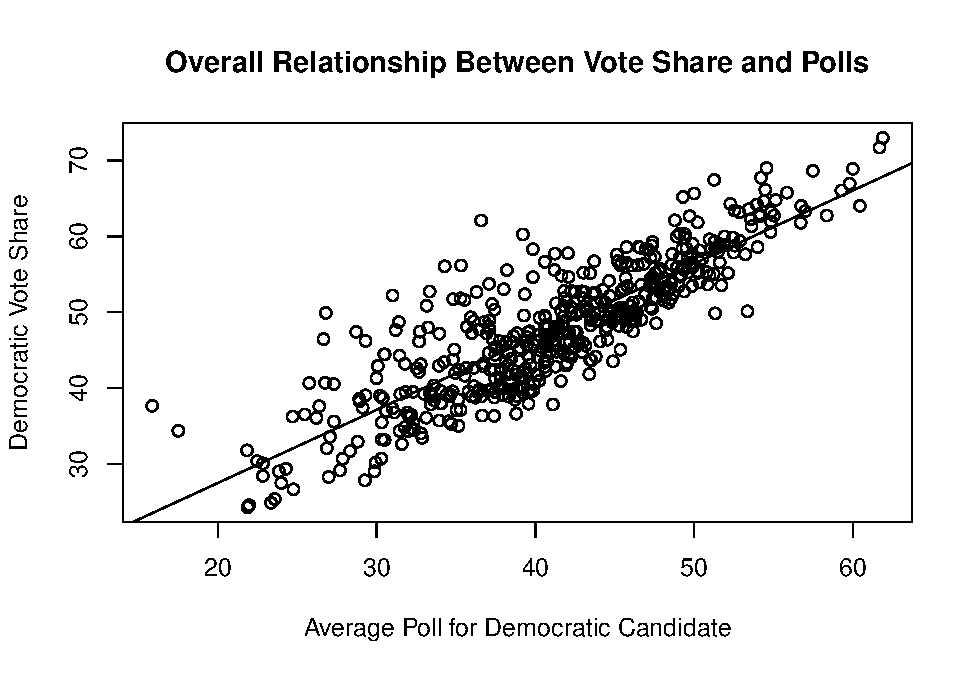
\includegraphics{blog_pred_files/figure-latex/unnamed-chunk-1-1.pdf}

\begin{Shaded}
\begin{Highlighting}[]
\CommentTok{# 2020 PREDICTION}
\NormalTok{pred_}\DecValTok{2020}\NormalTok{ <-}\StringTok{ }\KeywordTok{predict}\NormalTok{(fit_state_poll, }\DataTypeTok{newdata =}\NormalTok{ new_data_poll)}
\NormalTok{poll_pred_}\DecValTok{2020}\NormalTok{ <-}\StringTok{ }\KeywordTok{tibble}\NormalTok{(}\DataTypeTok{state =}\NormalTok{ new_data_poll}\OperatorTok{$}\NormalTok{state, }\DataTypeTok{pred =}\NormalTok{ pred_}\DecValTok{2020}\NormalTok{)}

\NormalTok{poll_pred_}\DecValTok{2020} \OperatorTok\StringTok{  }\CommentTok{##`statebins` needs state to be character, not factor!}
\StringTok{  }\KeywordTok{ggplot}\NormalTok{(}\KeywordTok{aes}\NormalTok{(}\DataTypeTok{state =}\NormalTok{ state, }\DataTypeTok{fill =}\NormalTok{ (pred }\OperatorTok{>=}\StringTok{ }\DecValTok{50}\NormalTok{))) }\OperatorTok{+}
\StringTok{  }\KeywordTok{geom_statebins}\NormalTok{() }\OperatorTok{+}
\StringTok{  }\KeywordTok{theme_statebins}\NormalTok{() }\OperatorTok{+}
\StringTok{  }\KeywordTok{labs}\NormalTok{(}\DataTypeTok{title =} \StringTok{"Poll Model: Electoral Vote Prediction"}\NormalTok{,}
       \DataTypeTok{subtitle =} \StringTok{"2020 Prediction"}\NormalTok{,}
       \DataTypeTok{fill =} \StringTok{""}\NormalTok{, }
       \DataTypeTok{caption =} \StringTok{"Date: FiveThirtyEight"}\NormalTok{) }\OperatorTok{+}
\StringTok{  }\KeywordTok{theme}\NormalTok{(}\DataTypeTok{legend.position =} \StringTok{"none"}\NormalTok{, }
        \DataTypeTok{plot.subtitle =} \KeywordTok{element_text}\NormalTok{(}\DataTypeTok{size =} \DecValTok{10}\NormalTok{, }\DataTypeTok{hjust =} \FloatTok{0.5}\NormalTok{),}
        \DataTypeTok{plot.title   =} \KeywordTok{element_text}\NormalTok{(}\DataTypeTok{size =} \DecValTok{12}\NormalTok{, }\DataTypeTok{hjust =} \FloatTok{0.5}\NormalTok{, }\DataTypeTok{face =} \StringTok{"bold"}\NormalTok{))}
\end{Highlighting}
\end{Shaded}

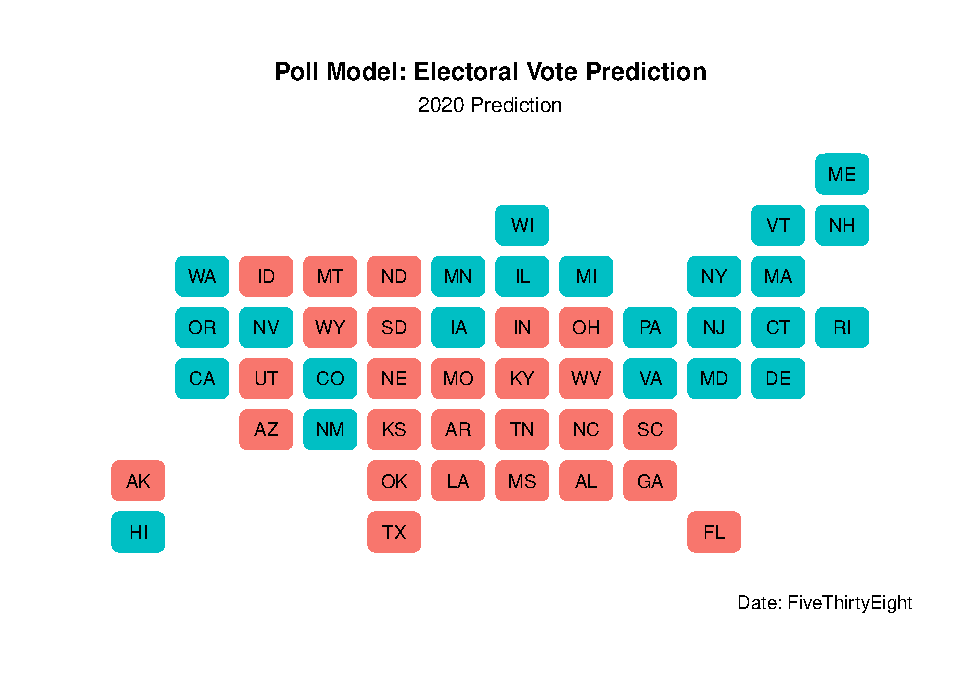
\includegraphics{blog_pred_files/figure-latex/unnamed-chunk-1-2.pdf}

\begin{Shaded}
\begin{Highlighting}[]
\NormalTok{poll_pred_}\DecValTok{2020}  \OperatorTok
\StringTok{  }\KeywordTok{select}\NormalTok{(state, pred) }\OperatorTok
\StringTok{  }\KeywordTok{mutate}\NormalTok{(}\DataTypeTok{state =}\NormalTok{  state.abb[}\KeywordTok{match}\NormalTok{(state,state.name)]) }\OperatorTok
\StringTok{  }\KeywordTok{left_join}\NormalTok{(electoral, }\DataTypeTok{by =} \StringTok{"state"}\NormalTok{) }\OperatorTok
\StringTok{  }\KeywordTok{mutate}\NormalTok{(}\DataTypeTok{state_win =} \KeywordTok{case_when}\NormalTok{(pred }\OperatorTok{>}\StringTok{ }\DecValTok{50} \OperatorTok{~}\StringTok{ "Biden"}\NormalTok{,}
\NormalTok{                            pred }\OperatorTok{<}\StringTok{ }\DecValTok{50} \OperatorTok{~}\StringTok{ "Trump"}\NormalTok{)) }\OperatorTok
\StringTok{  }\KeywordTok{group_by}\NormalTok{(state_win) }\OperatorTok
\StringTok{  }\KeywordTok{summarise}\NormalTok{(}\DataTypeTok{electoral_votes =} \KeywordTok{sum}\NormalTok{(}\StringTok{`}\DataTypeTok{2020}\StringTok{`}\NormalTok{)) }\OperatorTok
\StringTok{  }\KeywordTok{gt}\NormalTok{() }\OperatorTok
\StringTok{  }\KeywordTok{tab_header}\NormalTok{(}\DataTypeTok{title =} \KeywordTok{md}\NormalTok{(}\StringTok{"**2020 Electoral Vote Outcome Using Poll Model**"}\NormalTok{), }
               \DataTypeTok{subtitle =} \StringTok{"Biden Wins"}\NormalTok{) }\OperatorTok
\StringTok{   }\KeywordTok{cols_label}\NormalTok{(}\DataTypeTok{state_win =} \KeywordTok{md}\NormalTok{(}\StringTok{"**Candidate**"}\NormalTok{),}
               \DataTypeTok{electoral_votes =} \KeywordTok{md}\NormalTok{(}\StringTok{"**Total Electoral Votes**"}\NormalTok{)) }\OperatorTok
\StringTok{  }\KeywordTok{tab_source_note}\NormalTok{(}\KeywordTok{md}\NormalTok{(}\StringTok{"*Data: FiveThirtyEight*"}\NormalTok{)) }
\end{Highlighting}
\end{Shaded}

\begin{verbatim}
## `summarise()` ungrouping output (override with `.groups` argument)
\end{verbatim}

\captionsetup[table]{labelformat=empty,skip=1pt}
\begin{longtable}{lr}
\caption*{
\large \textbf{2020 Electoral Vote Outcome Using Poll Model}\\ 
\small Biden Wins\\ 
} \\ 
\toprule
\textbf{Candidate} & \textbf{Total Electoral Votes} \\ 
\midrule
Biden & 282 \\ 
Trump & 253 \\ 
\bottomrule
\end{longtable}
\begin{minipage}{\linewidth}
\emph{Data: FiveThirtyEight}\\ 
\end{minipage}

\hypertarget{demographics}{%
\section{DEMOGRAPHICS}\label{demographics}}

\begin{Shaded}
\begin{Highlighting}[]
\NormalTok{demog <-}\StringTok{ }\KeywordTok{read_csv}\NormalTok{(}\StringTok{"~/Desktop/R studio/carine-h.github.io/data/demographic_1990-2018.csv"}\NormalTok{)}
\end{Highlighting}
\end{Shaded}

\begin{verbatim}
## Parsed with column specification:
## cols(
##   year = col_double(),
##   state = col_character(),
##   Asian = col_double(),
##   Black = col_double(),
##   Hispanic = col_double(),
##   Indigenous = col_double(),
##   White = col_double(),
##   Female = col_double(),
##   Male = col_double(),
##   age20 = col_double(),
##   age3045 = col_double(),
##   age4565 = col_double(),
##   age65 = col_double(),
##   total = col_double()
## )
\end{verbatim}

\begin{Shaded}
\begin{Highlighting}[]
\NormalTok{pvstate_df    <-}\StringTok{ }\KeywordTok{read_csv}\NormalTok{(}\StringTok{"~/Desktop/R studio/carine-h.github.io/data/popvote_bystate_1948-2016.csv"}\NormalTok{)}
\end{Highlighting}
\end{Shaded}

\begin{verbatim}
## Parsed with column specification:
## cols(
##   state = col_character(),
##   year = col_double(),
##   total = col_double(),
##   D = col_double(),
##   R = col_double(),
##   R_pv2p = col_double(),
##   D_pv2p = col_double()
## )
\end{verbatim}

\begin{Shaded}
\begin{Highlighting}[]
\NormalTok{pollstate_df  <-}\StringTok{ }\KeywordTok{read_csv}\NormalTok{(}\StringTok{"~/Desktop/R studio/carine-h.github.io/data/pollavg_bystate_1968-2016.csv"}\NormalTok{)}
\end{Highlighting}
\end{Shaded}

\begin{verbatim}
## Parsed with column specification:
## cols(
##   year = col_double(),
##   state = col_character(),
##   party = col_character(),
##   candidate_name = col_character(),
##   poll_date = col_date(format = ""),
##   weeks_left = col_double(),
##   days_left = col_double(),
##   before_convention = col_logical(),
##   avg_poll = col_double()
## )
\end{verbatim}

\begin{Shaded}
\begin{Highlighting}[]
\NormalTok{hispanic_}\DecValTok{2020}\NormalTok{ <-}\StringTok{ }\KeywordTok{read_csv}\NormalTok{(}\StringTok{"~/Desktop/R studio/carine-h.github.io/data/csvData.csv"}\NormalTok{)}
\end{Highlighting}
\end{Shaded}

\begin{verbatim}
## Parsed with column specification:
## cols(
##   State = col_character(),
##   HispanicTotal = col_double(),
##   HispanicPerc = col_double()
## )
\end{verbatim}

\begin{Shaded}
\begin{Highlighting}[]
\NormalTok{race_}\DecValTok{2020}\NormalTok{ <-}\StringTok{ }\KeywordTok{read_csv}\NormalTok{(}\StringTok{"~/Desktop/R studio/carine-h.github.io/data/demog_race.csv"}\NormalTok{)}
\end{Highlighting}
\end{Shaded}

\begin{verbatim}
## Parsed with column specification:
## cols(
##   State = col_character(),
##   WhitePerc = col_double(),
##   BlackPerc = col_double(),
##   NativePerc = col_double(),
##   AsianPerc = col_double(),
##   IslanderPerc = col_double(),
##   OtherRacePerc = col_double(),
##   TwoOrMoreRacesPerc = col_double()
## )
\end{verbatim}

\begin{Shaded}
\begin{Highlighting}[]
\NormalTok{electoral_votes <-}\StringTok{ }\KeywordTok{read_csv}\NormalTok{(}\StringTok{"~/Desktop/R studio/carine-h.github.io/data/electoralcollegevotes_1948-2020.csv"}\NormalTok{)}
\end{Highlighting}
\end{Shaded}

\begin{verbatim}
## Warning: Missing column names filled in: 'X1' [1], 'X22' [22], 'X23' [23],
## 'X24' [24], 'X25' [25], 'X26' [26], 'X27' [27], 'X28' [28]
\end{verbatim}

\begin{verbatim}
## Parsed with column specification:
## cols(
##   .default = col_double(),
##   X1 = col_character(),
##   X22 = col_logical(),
##   X23 = col_logical(),
##   X24 = col_logical(),
##   X25 = col_logical(),
##   X26 = col_logical(),
##   X27 = col_logical(),
##   X28 = col_logical()
## )
\end{verbatim}

\begin{verbatim}
## See spec(...) for full column specifications.
\end{verbatim}

\begin{Shaded}
\begin{Highlighting}[]
\CommentTok{# state names and abbreviations}
\NormalTok{pvstate_df}\OperatorTok{$}\NormalTok{state <-}\StringTok{ }\NormalTok{state.abb[}\KeywordTok{match}\NormalTok{(pvstate_df}\OperatorTok{$}\NormalTok{state, state.name)]}
\NormalTok{pollstate_df}\OperatorTok{$}\NormalTok{state <-}\StringTok{ }\NormalTok{state.abb[}\KeywordTok{match}\NormalTok{(pollstate_df}\OperatorTok{$}\NormalTok{state, state.name)]}

\NormalTok{dat <-}\StringTok{ }\NormalTok{pvstate_df }\OperatorTok\StringTok{ }
\StringTok{  }\KeywordTok{full_join}\NormalTok{(pollstate_df }\OperatorTok\StringTok{ }
\StringTok{              }\KeywordTok{filter}\NormalTok{(weeks_left }\OperatorTok{==}\StringTok{ }\DecValTok{10}\NormalTok{) }\OperatorTok\StringTok{ }
\StringTok{              }\KeywordTok{group_by}\NormalTok{(year,party,state) }\OperatorTok\StringTok{ }
\StringTok{              }\KeywordTok{summarise}\NormalTok{(}\DataTypeTok{avg_poll=}\KeywordTok{mean}\NormalTok{(avg_poll)),}
            \DataTypeTok{by =} \KeywordTok{c}\NormalTok{(}\StringTok{"year"}\NormalTok{ ,}\StringTok{"state"}\NormalTok{)) }\OperatorTok
\StringTok{  }\KeywordTok{left_join}\NormalTok{(demog }\OperatorTok
\StringTok{              }\KeywordTok{select}\NormalTok{(}\OperatorTok{-}\KeywordTok{c}\NormalTok{(}\StringTok{"total"}\NormalTok{)),}
            \DataTypeTok{by =} \KeywordTok{c}\NormalTok{(}\StringTok{"year"}\NormalTok{ ,}\StringTok{"state"}\NormalTok{))}
\end{Highlighting}
\end{Shaded}

\begin{verbatim}
## `summarise()` regrouping output by 'year', 'party' (override with `.groups` argument)
\end{verbatim}

\begin{Shaded}
\begin{Highlighting}[]
\CommentTok{# demographics, poll numbers, and popular vote }

\NormalTok{dat}\OperatorTok{$}\NormalTok{region <-}\StringTok{ }\NormalTok{state.division[}\KeywordTok{match}\NormalTok{(dat}\OperatorTok{$}\NormalTok{state, state.abb)]}
\NormalTok{demog}\OperatorTok{$}\NormalTok{region <-}\StringTok{ }\NormalTok{state.division[}\KeywordTok{match}\NormalTok{(demog}\OperatorTok{$}\NormalTok{state, state.abb)]}

\NormalTok{dat_change <-}\StringTok{ }\NormalTok{dat }\OperatorTok
\StringTok{  }\KeywordTok{group_by}\NormalTok{(state) }\OperatorTok
\StringTok{  }\KeywordTok{mutate}\NormalTok{(}\DataTypeTok{Asian_change =}\NormalTok{ Asian }\OperatorTok{-}\StringTok{ }\KeywordTok{lag}\NormalTok{(Asian, }\DataTypeTok{order_by =}\NormalTok{ year),}
         \DataTypeTok{Black_change =}\NormalTok{ Black }\OperatorTok{-}\StringTok{ }\KeywordTok{lag}\NormalTok{(Black, }\DataTypeTok{order_by =}\NormalTok{ year),}
         \DataTypeTok{Hispanic_change =}\NormalTok{ Hispanic }\OperatorTok{-}\StringTok{ }\KeywordTok{lag}\NormalTok{(Hispanic, }\DataTypeTok{order_by =}\NormalTok{ year),}
         \DataTypeTok{Indigenous_change =}\NormalTok{ Indigenous }\OperatorTok{-}\StringTok{ }\KeywordTok{lag}\NormalTok{(Indigenous, }\DataTypeTok{order_by =}\NormalTok{ year),}
         \DataTypeTok{White_change =}\NormalTok{ White }\OperatorTok{-}\StringTok{ }\KeywordTok{lag}\NormalTok{(White, }\DataTypeTok{order_by =}\NormalTok{ year),}
         \DataTypeTok{Female_change =}\NormalTok{ Female }\OperatorTok{-}\StringTok{ }\KeywordTok{lag}\NormalTok{(Female, }\DataTypeTok{order_by =}\NormalTok{ year),}
         \DataTypeTok{Male_change =}\NormalTok{ Male }\OperatorTok{-}\StringTok{ }\KeywordTok{lag}\NormalTok{(Male, }\DataTypeTok{order_by =}\NormalTok{ year),}
         \DataTypeTok{age20_change =}\NormalTok{ age20 }\OperatorTok{-}\StringTok{ }\KeywordTok{lag}\NormalTok{(age20, }\DataTypeTok{order_by =}\NormalTok{ year),}
         \DataTypeTok{age3045_change =}\NormalTok{ age3045 }\OperatorTok{-}\StringTok{ }\KeywordTok{lag}\NormalTok{(age3045, }\DataTypeTok{order_by =}\NormalTok{ year),}
         \DataTypeTok{age4565_change =}\NormalTok{ age4565 }\OperatorTok{-}\StringTok{ }\KeywordTok{lag}\NormalTok{(age4565, }\DataTypeTok{order_by =}\NormalTok{ year),}
         \DataTypeTok{age65_change =}\NormalTok{ age65 }\OperatorTok{-}\StringTok{ }\KeywordTok{lag}\NormalTok{(age65, }\DataTypeTok{order_by =}\NormalTok{ year)}
\NormalTok{  )}



\CommentTok{## MODEL}
\NormalTok{mod_demog_change <-}\StringTok{ }\KeywordTok{lm}\NormalTok{(D_pv2p }\OperatorTok{~}\StringTok{ }\NormalTok{Black_change }\OperatorTok{+}\StringTok{ }\NormalTok{Hispanic_change }\OperatorTok{+}\StringTok{ }\NormalTok{Asian_change }\OperatorTok{+}
\StringTok{                         }\KeywordTok{as.factor}\NormalTok{(state), }\DataTypeTok{data =}\NormalTok{ dat_change)}



\CommentTok{# UPDATED 2020}
\NormalTok{dat_}\DecValTok{2020}\NormalTok{ <-}\StringTok{ }\NormalTok{race_}\DecValTok{2020} \OperatorTok
\StringTok{  }\KeywordTok{left_join}\NormalTok{(hispanic_}\DecValTok{2020}\NormalTok{, }\DataTypeTok{by =} \StringTok{"State"}\NormalTok{) }\OperatorTok
\StringTok{  }\KeywordTok{mutate}\NormalTok{(}\DataTypeTok{Hispanic =} \DecValTok{100}\OperatorTok{*}\NormalTok{HispanicPerc, }
         \DataTypeTok{state =}\NormalTok{ State, }
         \DataTypeTok{White =} \DecValTok{100}\OperatorTok{*}\NormalTok{WhitePerc, }
         \DataTypeTok{Asian =} \DecValTok{100}\OperatorTok{*}\NormalTok{AsianPerc, }
         \DataTypeTok{Black =} \DecValTok{100}\OperatorTok{*}\NormalTok{BlackPerc) }\OperatorTok
\StringTok{  }\KeywordTok{select}\NormalTok{(state, Hispanic, White, Asian, Black) }\OperatorTok
\StringTok{  }\KeywordTok{mutate}\NormalTok{(}\DataTypeTok{state =}\NormalTok{ state.abb[}\KeywordTok{match}\NormalTok{(state,state.name)]) }\OperatorTok
\StringTok{  }\KeywordTok{na.omit}\NormalTok{() }\OperatorTok
\StringTok{  }\KeywordTok{mutate}\NormalTok{(}\DataTypeTok{year =} \DecValTok{2020}\NormalTok{)}

\CommentTok{# 2018 demographics}
\NormalTok{dat_}\DecValTok{2018}\NormalTok{ <-}\StringTok{ }\NormalTok{demog }\OperatorTok
\StringTok{  }\KeywordTok{filter}\NormalTok{(year }\OperatorTok{==}\StringTok{ }\DecValTok{2018}\NormalTok{) }

\CommentTok{# joining demographics}
\NormalTok{real_}\DecValTok{2020}\NormalTok{_change <-}\StringTok{ }\KeywordTok{bind_rows}\NormalTok{(dat_}\DecValTok{2018}\NormalTok{, dat_}\DecValTok{2020}\NormalTok{)}

\CommentTok{# calculating percent changes in available demographic groups}
\CommentTok{## I used 0 percent change with populations that lacked demographic data (age and gender)}
\NormalTok{real_}\DecValTok{2020}\NormalTok{ <-}\StringTok{ }\NormalTok{real_}\DecValTok{2020}\NormalTok{_change }\OperatorTok
\StringTok{  }\KeywordTok{filter}\NormalTok{(year }\OperatorTok\StringTok{ }\KeywordTok{c}\NormalTok{(}\DecValTok{2018}\NormalTok{, }\DecValTok{2020}\NormalTok{)) }\OperatorTok
\StringTok{  }\KeywordTok{group_by}\NormalTok{(state) }\OperatorTok
\StringTok{  }\KeywordTok{mutate}\NormalTok{(}\DataTypeTok{Asian_change =}\NormalTok{ Asian }\OperatorTok{-}\StringTok{ }\KeywordTok{lag}\NormalTok{(Asian, }\DataTypeTok{order_by =}\NormalTok{ year), }\CommentTok{# CALCULATING CHANGES IN POPULATION}
         \DataTypeTok{Black_change =}\NormalTok{ Black }\OperatorTok{-}\StringTok{ }\KeywordTok{lag}\NormalTok{(Black, }\DataTypeTok{order_by =}\NormalTok{ year),}
         \DataTypeTok{Hispanic_change =}\NormalTok{ Hispanic }\OperatorTok{-}\StringTok{ }\KeywordTok{lag}\NormalTok{(Hispanic, }\DataTypeTok{order_by =}\NormalTok{ year),}
         \DataTypeTok{Indigenous_change =} \DecValTok{0}\NormalTok{,}
         \DataTypeTok{White_change =}\NormalTok{ White }\OperatorTok{-}\StringTok{ }\KeywordTok{lag}\NormalTok{(White, }\DataTypeTok{order_by =}\NormalTok{ year),}
         \DataTypeTok{Female_change =} \DecValTok{0}\NormalTok{,}
         \DataTypeTok{Male_change =} \DecValTok{0}\NormalTok{,}
         \DataTypeTok{age20_change =} \DecValTok{0}\NormalTok{,}
         \DataTypeTok{age3045_change =} \DecValTok{0}\NormalTok{,}
         \DataTypeTok{age4565_change =} \DecValTok{0}\NormalTok{,}
         \DataTypeTok{age65_change =} \DecValTok{0}\NormalTok{) }\OperatorTok
\StringTok{  }\KeywordTok{filter}\NormalTok{(year }\OperatorTok{==}\StringTok{ }\DecValTok{2020}\NormalTok{)}

\NormalTok{real_}\DecValTok{2020}\NormalTok{ <-}\StringTok{ }\KeywordTok{as.data.frame}\NormalTok{(real_}\DecValTok{2020}\NormalTok{)}
\KeywordTok{rownames}\NormalTok{(real_}\DecValTok{2020}\NormalTok{) <-}\StringTok{ }\NormalTok{real_}\DecValTok{2020}\OperatorTok{$}\NormalTok{state}
\NormalTok{real_}\DecValTok{2020}\NormalTok{ <-}\StringTok{ }\NormalTok{real_}\DecValTok{2020}\NormalTok{[state.abb, ]}
\NormalTok{real_}\DecValTok{2020}\OperatorTok{$}\NormalTok{region <-}\StringTok{ }\NormalTok{state.division[}\KeywordTok{match}\NormalTok{(real_}\DecValTok{2020}\OperatorTok{$}\NormalTok{state, state.abb)]}

\CommentTok{#  2020 PREDICTION}
\NormalTok{demog_pred <-}\StringTok{ }\KeywordTok{predict}\NormalTok{(mod_demog_change, }\DataTypeTok{newdata =}\NormalTok{ real_}\DecValTok{2020}\NormalTok{) }

\NormalTok{d <-}\StringTok{ }\KeywordTok{tibble}\NormalTok{(demog_pred) }\OperatorTok
\StringTok{  }\KeywordTok{mutate}\NormalTok{(}\DataTypeTok{state =}\NormalTok{ real_}\DecValTok{2020}\OperatorTok{$}\NormalTok{state)}


\NormalTok{ d}\OperatorTok\StringTok{  }\CommentTok{##`statebins` needs state to be character, not factor!}
\StringTok{  }\KeywordTok{ggplot}\NormalTok{(}\KeywordTok{aes}\NormalTok{(}\DataTypeTok{state =}\NormalTok{ state, }\DataTypeTok{fill =}\NormalTok{ (demog_pred }\OperatorTok{>=}\StringTok{ }\DecValTok{50}\NormalTok{))) }\OperatorTok{+}
\StringTok{  }\KeywordTok{geom_statebins}\NormalTok{() }\OperatorTok{+}
\StringTok{  }\KeywordTok{theme_statebins}\NormalTok{() }\OperatorTok{+}
\StringTok{  }\KeywordTok{labs}\NormalTok{(}\DataTypeTok{title =} \StringTok{"Demographic Model: Electoral Vote Prediction"}\NormalTok{,}
       \DataTypeTok{subtitle =} \StringTok{"2020 Prediction"}\NormalTok{,}
       \DataTypeTok{fill =} \StringTok{""}\NormalTok{, }
       \DataTypeTok{caption =} \StringTok{"Data: World Population Review"}\NormalTok{) }\OperatorTok{+}
\StringTok{  }\KeywordTok{theme}\NormalTok{(}\DataTypeTok{legend.position =} \StringTok{"none"}\NormalTok{, }
        \DataTypeTok{plot.subtitle =} \KeywordTok{element_text}\NormalTok{(}\DataTypeTok{size =} \DecValTok{10}\NormalTok{, }\DataTypeTok{hjust =} \FloatTok{0.5}\NormalTok{),}
        \DataTypeTok{plot.title   =} \KeywordTok{element_text}\NormalTok{(}\DataTypeTok{size =} \DecValTok{12}\NormalTok{, }\DataTypeTok{hjust =} \FloatTok{0.5}\NormalTok{, }\DataTypeTok{face =} \StringTok{"bold"}\NormalTok{))}
\end{Highlighting}
\end{Shaded}

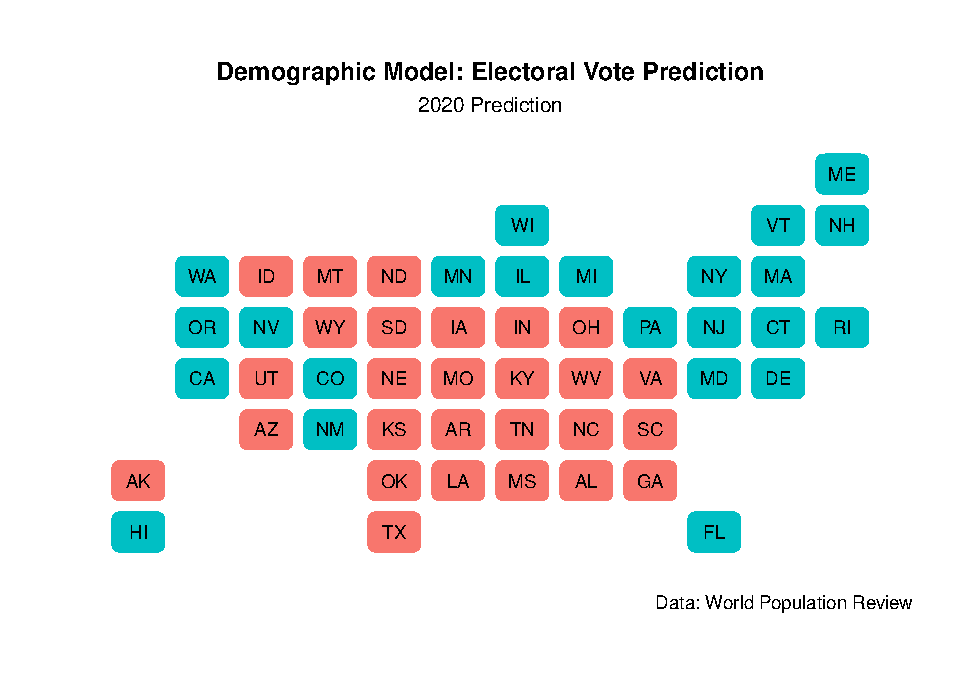
\includegraphics{blog_pred_files/figure-latex/unnamed-chunk-2-1.pdf}

\begin{Shaded}
\begin{Highlighting}[]
\NormalTok{d }\OperatorTok
\StringTok{  }\KeywordTok{select}\NormalTok{(state, demog_pred) }\OperatorTok
\StringTok{  }\KeywordTok{left_join}\NormalTok{(electoral, }\DataTypeTok{by =} \StringTok{"state"}\NormalTok{) }\OperatorTok
\StringTok{  }\KeywordTok{mutate}\NormalTok{(}\DataTypeTok{state_win =} \KeywordTok{case_when}\NormalTok{(demog_pred }\OperatorTok{>}\StringTok{ }\DecValTok{50} \OperatorTok{~}\StringTok{ "Biden"}\NormalTok{,}
\NormalTok{                            demog_pred }\OperatorTok{<}\StringTok{ }\DecValTok{50} \OperatorTok{~}\StringTok{ "Trump"}\NormalTok{)) }\OperatorTok
\StringTok{  }\KeywordTok{group_by}\NormalTok{(state_win) }\OperatorTok
\StringTok{  }\KeywordTok{summarise}\NormalTok{(}\DataTypeTok{electoral_votes =} \KeywordTok{sum}\NormalTok{(}\StringTok{`}\DataTypeTok{2020}\StringTok{`}\NormalTok{)) }\OperatorTok
\StringTok{  }\KeywordTok{gt}\NormalTok{() }\OperatorTok
\StringTok{  }\KeywordTok{tab_header}\NormalTok{(}\DataTypeTok{title =} \KeywordTok{md}\NormalTok{(}\StringTok{"**2020 Electoral Vote Outcome Using Demographic Model**"}\NormalTok{), }
               \DataTypeTok{subtitle =} \StringTok{"Biden Wins"}\NormalTok{) }\OperatorTok
\StringTok{   }\KeywordTok{cols_label}\NormalTok{(}\DataTypeTok{state_win =} \KeywordTok{md}\NormalTok{(}\StringTok{"**Candidate**"}\NormalTok{),}
               \DataTypeTok{electoral_votes =} \KeywordTok{md}\NormalTok{(}\StringTok{"**Total Electoral Votes**"}\NormalTok{)) }\OperatorTok
\StringTok{  }\KeywordTok{tab_source_note}\NormalTok{(}\KeywordTok{md}\NormalTok{(}\StringTok{"*Data: World Population Review*"}\NormalTok{)) }
\end{Highlighting}
\end{Shaded}

\begin{verbatim}
## `summarise()` ungrouping output (override with `.groups` argument)
\end{verbatim}

\captionsetup[table]{labelformat=empty,skip=1pt}
\begin{longtable}{lr}
\caption*{
\large \textbf{2020 Electoral Vote Outcome Using Demographic Model}\\ 
\small Biden Wins\\ 
} \\ 
\toprule
\textbf{Candidate} & \textbf{Total Electoral Votes} \\ 
\midrule
Biden & 292 \\ 
Trump & 243 \\ 
\bottomrule
\end{longtable}
\begin{minipage}{\linewidth}
\emph{Data: World Population Review}\\ 
\end{minipage}

\hypertarget{economics}{%
\section{ECONOMICS}\label{economics}}

\begin{Shaded}
\begin{Highlighting}[]
\KeywordTok{library}\NormalTok{(readxl)}
\NormalTok{q2_}\DecValTok{2020}\NormalTok{ <-}\StringTok{ }\KeywordTok{read_excel}\NormalTok{(}\StringTok{"pred_data/q2_2020.xlsx"}\NormalTok{) }\OperatorTok
\StringTok{  }\KeywordTok{na.omit}\NormalTok{()}\OperatorTok
\StringTok{  }\KeywordTok{mutate}\NormalTok{(}\DataTypeTok{state =}\NormalTok{ state.abb[}\KeywordTok{match}\NormalTok{(state,state.name)])}
\NormalTok{state_gdp <-}\StringTok{ }\KeywordTok{read_csv}\NormalTok{(}\StringTok{"pred_data/state_gdp_quarter.csv"}\NormalTok{)}
\end{Highlighting}
\end{Shaded}

\begin{verbatim}
## Parsed with column specification:
## cols(
##   GeoFIPS = col_character(),
##   GeoName = col_character(),
##   Region = col_double(),
##   TableName = col_character(),
##   LineCode = col_double(),
##   IndustryClassification = col_character(),
##   Description = col_character(),
##   Unit = col_character(),
##   `2008` = col_double(),
##   `2009` = col_double(),
##   `2010` = col_double(),
##   `2011` = col_double(),
##   `2012` = col_double(),
##   `2013` = col_double(),
##   `2014` = col_double(),
##   `2015` = col_double(),
##   `2016` = col_double(),
##   `2017` = col_double(),
##   `2018` = col_double()
## )
\end{verbatim}

\begin{verbatim}
## Warning: 4 parsing failures.
## row col   expected    actual                              file
## 209  -- 19 columns 1 columns 'pred_data/state_gdp_quarter.csv'
## 210  -- 19 columns 1 columns 'pred_data/state_gdp_quarter.csv'
## 211  -- 19 columns 1 columns 'pred_data/state_gdp_quarter.csv'
## 212  -- 19 columns 1 columns 'pred_data/state_gdp_quarter.csv'
\end{verbatim}

\begin{Shaded}
\begin{Highlighting}[]
\NormalTok{econ_update}
\end{Highlighting}
\end{Shaded}

\begin{verbatim}
## # A tibble: 484 x 31
##    GeoFIPS GeoName Region TableName LineCode IndustryClassif~ Description Unit 
##    <chr>   <chr>    <dbl> <chr>        <dbl> <chr>            <chr>       <chr>
##  1 00000   United~     NA SAGDP1           1 ...              Real GDP (~ Mill~
##  2 00000   United~     NA SAGDP1           2 ...              Chain-type~ Quan~
##  3 00000   United~     NA SAGDP1           3 ...              Current-do~ Mill~
##  4 00000   United~     NA SAGDP1           4 ...              Compensati~ Mill~
##  5 00000   United~     NA SAGDP1           5 ...              Gross oper~ Mill~
##  6 00000   United~     NA SAGDP1           6 ...              Taxes on p~ Mill~
##  7 00000   United~     NA SAGDP1           7 ...              Taxes on p~ Mill~
##  8 00000   United~     NA SAGDP1           8 ...              Subsidies ~ Mill~
##  9 01000   Alabama      5 SAGDP1           1 ...              Real GDP (~ Mill~
## 10 01000   Alabama      5 SAGDP1           2 ...              Chain-type~ Quan~
## # ... with 474 more rows, and 23 more variables: `1997` <dbl>, `1998` <dbl>,
## #   `1999` <dbl>, `2000` <dbl>, `2001` <dbl>, `2002` <dbl>, `2003` <dbl>,
## #   `2004` <dbl>, `2005` <dbl>, `2006` <dbl>, `2007` <dbl>, `2008` <dbl>,
## #   `2009` <dbl>, `2010` <dbl>, `2011` <dbl>, `2012` <dbl>, `2013` <dbl>,
## #   `2014` <dbl>, `2015` <dbl>, `2016` <dbl>, `2017` <dbl>, `2018` <dbl>,
## #   `2019` <dbl>
\end{verbatim}

\begin{Shaded}
\begin{Highlighting}[]
\CommentTok{# going to have to use yearly growth}
\NormalTok{state_econ <-}\StringTok{ }\NormalTok{econ_update }\OperatorTok
\StringTok{  }\KeywordTok{filter}\NormalTok{(Description }\OperatorTok{==}\StringTok{ "Real GDP (millions of chained 2012 dollars)"}\NormalTok{) }\OperatorTok
\StringTok{  }\KeywordTok{select}\NormalTok{(GeoName, }\StringTok{'1997'}\NormalTok{, }\StringTok{'1998'}\NormalTok{, }\StringTok{'1999'}\NormalTok{,}\StringTok{'2000'}\NormalTok{, }\StringTok{'2001'}\NormalTok{, }\StringTok{'2002'}\NormalTok{, }\StringTok{'2003'}\NormalTok{, }\StringTok{'2004'}\NormalTok{, }\StringTok{'2005'}\NormalTok{, }\StringTok{'2006'}\NormalTok{, }\StringTok{'2007'}\NormalTok{, }\StringTok{'2008'}\NormalTok{, }\StringTok{'2009'}\NormalTok{, }\StringTok{'2010'}\NormalTok{, }\StringTok{'2011'}\NormalTok{, }\StringTok{'2012'}\NormalTok{, }\StringTok{'2013'}\NormalTok{, }\StringTok{'2014'}\NormalTok{, }\StringTok{'2015'}\NormalTok{, }\StringTok{'2016'}\NormalTok{, }\StringTok{'2017'}\NormalTok{, }\StringTok{'2018'}\NormalTok{)}\OperatorTok
\StringTok{  }\KeywordTok{melt}\NormalTok{(}\KeywordTok{c}\NormalTok{(}\StringTok{"GeoName"}\NormalTok{), }\DataTypeTok{value.name =} \StringTok{"GDP"}\NormalTok{) }\OperatorTok
\StringTok{  }\KeywordTok{mutate}\NormalTok{(}\DataTypeTok{year =} \KeywordTok{as.numeric}\NormalTok{(}\KeywordTok{as.character}\NormalTok{(variable))) }\OperatorTok
\StringTok{  }\KeywordTok{rename}\NormalTok{(}\DataTypeTok{state =}\NormalTok{ GeoName) }\OperatorTok
\StringTok{  }\KeywordTok{group_by}\NormalTok{(state) }\OperatorTok
\StringTok{  }\KeywordTok{mutate}\NormalTok{(}\DataTypeTok{gdp_growth=}\NormalTok{ (GDP }\OperatorTok{-}\StringTok{ }\KeywordTok{lag}\NormalTok{(GDP, }\DataTypeTok{order_by =}\NormalTok{ year))}\OperatorTok{/}\KeywordTok{lag}\NormalTok{(GDP, }\DataTypeTok{order_by =}\NormalTok{ year)) }\OperatorTok
\StringTok{  }\KeywordTok{mutate}\NormalTok{(}\DataTypeTok{state =}\NormalTok{ state.abb[}\KeywordTok{match}\NormalTok{(state,state.name)]) }\OperatorTok
\StringTok{  }\KeywordTok{select}\NormalTok{(year, state, gdp_growth) }\OperatorTok
\StringTok{  }\KeywordTok{na.omit}\NormalTok{()}
  


\NormalTok{q3_econ <-}\StringTok{ }\NormalTok{pvstate_df }\OperatorTok
\StringTok{  }\KeywordTok{left_join}\NormalTok{(state_econ, }\DataTypeTok{by =} \KeywordTok{c}\NormalTok{(}\StringTok{"year"}\NormalTok{, }\StringTok{"state"}\NormalTok{)) }\OperatorTok
\StringTok{  }\KeywordTok{left_join}\NormalTok{(popvote_df, }\DataTypeTok{by =} \KeywordTok{c}\NormalTok{(}\StringTok{"year"}\NormalTok{)) }\OperatorTok
\StringTok{  }\KeywordTok{na.omit}\NormalTok{() }\OperatorTok
\StringTok{  }\KeywordTok{filter}\NormalTok{(party }\OperatorTok{==}\StringTok{ "democrat"}\NormalTok{)}

\CommentTok{# MODEL}
\NormalTok{econ_fit <-}\StringTok{ }\KeywordTok{lm}\NormalTok{(D_pv2p }\OperatorTok{~}\StringTok{ }\NormalTok{gdp_growth}\OperatorTok{*}\NormalTok{incumbent }\OperatorTok{+}\StringTok{ }\KeywordTok{as.factor}\NormalTok{(state), }\DataTypeTok{data =}\NormalTok{ q3_econ)}
\KeywordTok{summary}\NormalTok{(econ_fit)}
\end{Highlighting}
\end{Shaded}

\begin{verbatim}
## 
## Call:
## lm(formula = D_pv2p ~ gdp_growth * incumbent + as.factor(state), 
##     data = q3_econ)
## 
## Residuals:
##      Min       1Q   Median       3Q      Max 
## -12.1919  -1.9037   0.0077   1.9924  10.7792 
## 
## Coefficients:
##                          Estimate Std. Error t value Pr(>|t|)    
## (Intercept)               38.1650     1.5989  23.870  < 2e-16 ***
## gdp_growth               -29.9112     9.3138  -3.211 0.001542 ** 
## incumbentTRUE              0.3537     0.6640   0.533 0.594849    
## as.factor(state)AL         0.8672     2.2617   0.383 0.701828    
## as.factor(state)AR         3.2325     2.2585   1.431 0.153933    
## as.factor(state)AZ         8.4376     2.2607   3.732 0.000248 ***
## as.factor(state)CA        22.9524     2.2720  10.102  < 2e-16 ***
## as.factor(state)CO        13.0791     2.2651   5.774 2.97e-08 ***
## as.factor(state)CT        20.8874     2.2696   9.203  < 2e-16 ***
## as.factor(state)DE        19.4663     2.2588   8.618 2.21e-15 ***
## as.factor(state)FL        12.0844     2.2634   5.339 2.56e-07 ***
## as.factor(state)GA         7.5603     2.2606   3.344 0.000987 ***
## as.factor(state)HI        27.7259     2.2649  12.242  < 2e-16 ***
## as.factor(state)IA        12.8317     2.2594   5.679 4.80e-08 ***
## as.factor(state)ID        -4.4666     2.2993  -1.943 0.053488 .  
## as.factor(state)IL        20.3558     2.2539   9.031  < 2e-16 ***
## as.factor(state)IN         5.6256     2.2621   2.487 0.013716 *  
## as.factor(state)KS         1.5380     2.2600   0.681 0.496974    
## as.factor(state)KY         1.1419     2.2530   0.507 0.612824    
## as.factor(state)LA         3.8342     2.2568   1.699 0.090905 .  
## as.factor(state)MA        25.9295     2.2663  11.441  < 2e-16 ***
## as.factor(state)MD        23.6211     2.2718  10.397  < 2e-16 ***
## as.factor(state)ME        17.5037     2.2669   7.722 5.67e-13 ***
## as.factor(state)MI        15.1378     2.2516   6.723 1.88e-10 ***
## as.factor(state)MN        15.1504     2.2688   6.678 2.42e-10 ***
## as.factor(state)MO         8.1954     2.2591   3.628 0.000364 ***
## as.factor(state)MS         4.2262     2.2585   1.871 0.062793 .  
## as.factor(state)MT         3.3494     2.2556   1.485 0.139161    
## as.factor(state)NC         9.3230     2.2665   4.113 5.73e-05 ***
## as.factor(state)ND        -0.9875     2.3214  -0.425 0.671019    
## as.factor(state)NE        -0.6513     2.2617  -0.288 0.773659    
## as.factor(state)NH        13.9894     2.2645   6.178 3.66e-09 ***
## as.factor(state)NJ        19.4069     2.2597   8.588 2.67e-15 ***
## as.factor(state)NM        15.7163     2.2618   6.949 5.26e-11 ***
## as.factor(state)NV        14.2156     2.2783   6.240 2.63e-09 ***
## as.factor(state)NY        25.7505     2.2522  11.433  < 2e-16 ***
## as.factor(state)OH        11.3059     2.2555   5.013 1.19e-06 ***
## as.factor(state)OK        -3.5304     2.2546  -1.566 0.118988    
## as.factor(state)OR        17.5964     2.2895   7.686 7.04e-13 ***
## as.factor(state)PA        14.4452     2.2594   6.393 1.15e-09 ***
## as.factor(state)RI        24.6834     2.2584  10.930  < 2e-16 ***
## as.factor(state)SC         5.3597     2.2594   2.372 0.018645 *  
## as.factor(state)SD         2.1645     2.2698   0.954 0.341458    
## as.factor(state)TN         4.0860     2.2573   1.810 0.071806 .  
## as.factor(state)TX         4.0057     2.2568   1.775 0.077453 .  
## as.factor(state)UT        -6.8451     2.2667  -3.020 0.002864 ** 
## as.factor(state)VA        12.3160     2.2645   5.439 1.58e-07 ***
## as.factor(state)VT        26.1969     2.2717  11.532  < 2e-16 ***
## as.factor(state)WA        18.5109     2.2554   8.207 2.91e-14 ***
## as.factor(state)WI        14.1764     2.2562   6.283 2.08e-09 ***
## as.factor(state)WV         1.4166     2.2573   0.628 0.531019    
## as.factor(state)WY        -8.6865     2.2701  -3.826 0.000175 ***
## gdp_growth:incumbentTRUE  40.8028    19.5016   2.092 0.037694 *  
## ---
## Signif. codes:  0 '***' 0.001 '**' 0.01 '*' 0.05 '.' 0.1 ' ' 1
## 
## Residual standard error: 3.555 on 197 degrees of freedom
## Multiple R-squared:  0.8985, Adjusted R-squared:  0.8717 
## F-statistic: 33.55 on 52 and 197 DF,  p-value: < 2.2e-16
\end{verbatim}

\begin{Shaded}
\begin{Highlighting}[]
\NormalTok{e <-}\StringTok{ }\NormalTok{econ_update }\OperatorTok
\StringTok{  }\KeywordTok{filter}\NormalTok{(Description }\OperatorTok{==}\StringTok{ "Real GDP (millions of chained 2012 dollars)"}\NormalTok{) }\OperatorTok
\StringTok{  }\KeywordTok{select}\NormalTok{(GeoName, }\StringTok{'1997'}\NormalTok{, }\StringTok{'1998'}\NormalTok{, }\StringTok{'1999'}\NormalTok{,}\StringTok{'2000'}\NormalTok{, }\StringTok{'2001'}\NormalTok{, }\StringTok{'2002'}\NormalTok{, }\StringTok{'2003'}\NormalTok{, }\StringTok{'2004'}\NormalTok{, }\StringTok{'2005'}\NormalTok{, }\StringTok{'2006'}\NormalTok{, }\StringTok{'2007'}\NormalTok{, }\StringTok{'2008'}\NormalTok{, }\StringTok{'2009'}\NormalTok{, }\StringTok{'2010'}\NormalTok{, }\StringTok{'2011'}\NormalTok{, }\StringTok{'2012'}\NormalTok{, }\StringTok{'2013'}\NormalTok{, }\StringTok{'2014'}\NormalTok{, }\StringTok{'2015'}\NormalTok{, }\StringTok{'2016'}\NormalTok{, }\StringTok{'2017'}\NormalTok{, }\StringTok{'2018'}\NormalTok{)}\OperatorTok
\StringTok{  }\KeywordTok{melt}\NormalTok{(}\KeywordTok{c}\NormalTok{(}\StringTok{"GeoName"}\NormalTok{), }\DataTypeTok{value.name =} \StringTok{"GDP"}\NormalTok{) }\OperatorTok
\StringTok{  }\KeywordTok{mutate}\NormalTok{(}\DataTypeTok{year =} \KeywordTok{as.numeric}\NormalTok{(}\KeywordTok{as.character}\NormalTok{(variable))) }\OperatorTok
\StringTok{  }\KeywordTok{rename}\NormalTok{(}\DataTypeTok{state =}\NormalTok{ GeoName) }\OperatorTok
\StringTok{  }\KeywordTok{mutate}\NormalTok{(}\DataTypeTok{state =}\NormalTok{ state.abb[}\KeywordTok{match}\NormalTok{(state,state.name)]) }\OperatorTok
\StringTok{  }\KeywordTok{select}\NormalTok{(state, year, GDP) }\OperatorTok
\StringTok{  }\KeywordTok{filter}\NormalTok{(year }\OperatorTok{==}\StringTok{ }\DecValTok{2018}\NormalTok{)}


\NormalTok{gdp_}\DecValTok{2019}\NormalTok{ <-}\StringTok{ }\KeywordTok{read_excel}\NormalTok{(}\StringTok{"pred_data/state_2019_gdp.xlsx"}\NormalTok{)}\OperatorTok
\StringTok{  }\KeywordTok{na.omit}\NormalTok{()}\OperatorTok
\StringTok{  }\KeywordTok{mutate}\NormalTok{(}\DataTypeTok{state =}\NormalTok{ state.abb[}\KeywordTok{match}\NormalTok{(state,state.name)]) }\OperatorTok
\StringTok{  }\KeywordTok{mutate}\NormalTok{(}\DataTypeTok{year =} \DecValTok{2019}\NormalTok{)}

\CommentTok{# new data: ASSUMING SAME GDP GROWTH ACROSS STATES AS IS NATIONALLY }
\NormalTok{data_econ <-}\StringTok{ }\NormalTok{q2_}\DecValTok{2020} \OperatorTok
\StringTok{  }\KeywordTok{mutate}\NormalTok{(}\DataTypeTok{year =} \DecValTok{2020}\NormalTok{) }

\NormalTok{new_data_econ <-}\StringTok{ }\KeywordTok{rbind}\NormalTok{(data_econ, gdp_}\DecValTok{2019}\NormalTok{) }\OperatorTok
\StringTok{  }\KeywordTok{mutate}\NormalTok{(}\DataTypeTok{incumbent =} \OtherTok{FALSE}\NormalTok{) }\OperatorTok
\StringTok{  }\KeywordTok{group_by}\NormalTok{(state) }\OperatorTok
\StringTok{  }\KeywordTok{mutate}\NormalTok{(}\DataTypeTok{gdp_growth =}\NormalTok{ (GDP }\OperatorTok{-}\StringTok{ }\KeywordTok{lag}\NormalTok{(GDP, }\DataTypeTok{order_by =}\NormalTok{ year))}\OperatorTok{/}\KeywordTok{lag}\NormalTok{(GDP, }\DataTypeTok{order_by =}\NormalTok{ year)) }\OperatorTok
\StringTok{  }\KeywordTok{na.omit}\NormalTok{()}
  

\CommentTok{# 2020 PREDICTION}
\NormalTok{econ_pred <-}\StringTok{ }\KeywordTok{predict}\NormalTok{(econ_fit, }\DataTypeTok{newdata =}\NormalTok{ new_data_econ)}

\NormalTok{e2 <-}\StringTok{ }\KeywordTok{tibble}\NormalTok{(}\DataTypeTok{pred =} \KeywordTok{predict}\NormalTok{(econ_fit, }\DataTypeTok{newdata =}\NormalTok{ new_data_econ), }\DataTypeTok{state =}\NormalTok{ new_data_econ}\OperatorTok{$}\NormalTok{state)}

\NormalTok{e2 }\OperatorTok\StringTok{  }\CommentTok{##`statebins` needs state to be character, not factor!}
\StringTok{  }\KeywordTok{ggplot}\NormalTok{(}\KeywordTok{aes}\NormalTok{(}\DataTypeTok{state =}\NormalTok{ state, }\DataTypeTok{fill =}\NormalTok{ (pred }\OperatorTok{>=}\StringTok{ }\DecValTok{50}\NormalTok{))) }\OperatorTok{+}
\StringTok{  }\KeywordTok{geom_statebins}\NormalTok{() }\OperatorTok{+}
\StringTok{  }\KeywordTok{theme_statebins}\NormalTok{() }\OperatorTok{+}
\StringTok{  }\KeywordTok{labs}\NormalTok{(}\DataTypeTok{title =} \StringTok{"Fundamentals Model: Electoral Vote Prediction"}\NormalTok{,}
       \DataTypeTok{subtitle =} \StringTok{"2020 Prediction"}\NormalTok{,}
       \DataTypeTok{fill =} \StringTok{""}\NormalTok{, }
       \DataTypeTok{caption =} \StringTok{"Data: BEA"}\NormalTok{) }\OperatorTok{+}
\StringTok{  }\KeywordTok{theme}\NormalTok{(}\DataTypeTok{legend.position =} \StringTok{"none"}\NormalTok{, }
        \DataTypeTok{plot.subtitle =} \KeywordTok{element_text}\NormalTok{(}\DataTypeTok{size =} \DecValTok{10}\NormalTok{, }\DataTypeTok{hjust =} \FloatTok{0.5}\NormalTok{),}
        \DataTypeTok{plot.title   =} \KeywordTok{element_text}\NormalTok{(}\DataTypeTok{size =} \DecValTok{12}\NormalTok{, }\DataTypeTok{hjust =} \FloatTok{0.5}\NormalTok{, }\DataTypeTok{face =} \StringTok{"bold"}\NormalTok{))}
\end{Highlighting}
\end{Shaded}

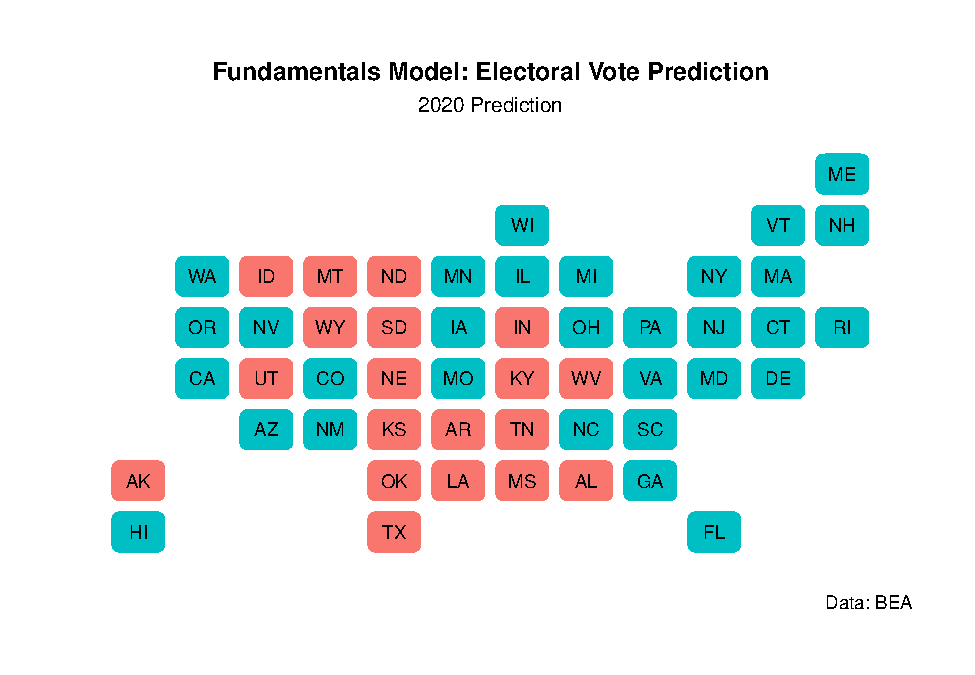
\includegraphics{blog_pred_files/figure-latex/unnamed-chunk-3-1.pdf}

\begin{Shaded}
\begin{Highlighting}[]
\NormalTok{e2  }\OperatorTok
\StringTok{  }\KeywordTok{select}\NormalTok{(state, pred) }\OperatorTok
\StringTok{  }\KeywordTok{left_join}\NormalTok{(electoral, }\DataTypeTok{by =} \StringTok{"state"}\NormalTok{) }\OperatorTok
\StringTok{  }\KeywordTok{mutate}\NormalTok{(}\DataTypeTok{state_win =} \KeywordTok{case_when}\NormalTok{(pred }\OperatorTok{>}\StringTok{ }\DecValTok{50} \OperatorTok{~}\StringTok{ "Biden"}\NormalTok{,}
\NormalTok{                            pred }\OperatorTok{<}\StringTok{ }\DecValTok{50} \OperatorTok{~}\StringTok{ "Trump"}\NormalTok{)) }\OperatorTok
\StringTok{  }\KeywordTok{group_by}\NormalTok{(state_win) }\OperatorTok
\StringTok{  }\KeywordTok{summarise}\NormalTok{(}\DataTypeTok{electoral_votes =} \KeywordTok{sum}\NormalTok{(}\StringTok{`}\DataTypeTok{2020}\StringTok{`}\NormalTok{)) }\OperatorTok
\StringTok{  }\KeywordTok{gt}\NormalTok{() }\OperatorTok
\StringTok{  }\KeywordTok{tab_header}\NormalTok{(}\DataTypeTok{title =} \KeywordTok{md}\NormalTok{(}\StringTok{"**2020 Electoral Vote Outcome Using Fundamentals Model**"}\NormalTok{), }
               \DataTypeTok{subtitle =} \StringTok{"Biden Wins"}\NormalTok{) }\OperatorTok
\StringTok{   }\KeywordTok{cols_label}\NormalTok{(}\DataTypeTok{state_win =} \KeywordTok{md}\NormalTok{(}\StringTok{"**Candidate**"}\NormalTok{),}
               \DataTypeTok{electoral_votes =} \KeywordTok{md}\NormalTok{(}\StringTok{"**Total Electoral Votes**"}\NormalTok{)) }\OperatorTok
\StringTok{  }\KeywordTok{tab_source_note}\NormalTok{(}\KeywordTok{md}\NormalTok{(}\StringTok{"*Data: FiveThirtyEight, BEA*"}\NormalTok{)) }
\end{Highlighting}
\end{Shaded}

\begin{verbatim}
## `summarise()` ungrouping output (override with `.groups` argument)
\end{verbatim}

\captionsetup[table]{labelformat=empty,skip=1pt}
\begin{longtable}{lr}
\caption*{
\large \textbf{2020 Electoral Vote Outcome Using Fundamentals Model}\\ 
\small Biden Wins\\ 
} \\ 
\toprule
\textbf{Candidate} & \textbf{Total Electoral Votes} \\ 
\midrule
Biden & 390 \\ 
Trump & 145 \\ 
\bottomrule
\end{longtable}
\begin{minipage}{\linewidth}
\emph{Data: FiveThirtyEight, BEA}\\ 
\end{minipage}

\hypertarget{plot-of-all-models}{%
\section{PLOT of ALL MODELS}\label{plot-of-all-models}}

in\_sample\_poll \textless- predict(fit\_state\_poll, newdata = dat)
in\_sample\_demo \textless- predict(mod\_demog\_change, newdata =
dat\_change) in\_sample\_econ \textless- predict(econ\_fit, newdata =
q3\_econ)

\hypertarget{ensemble}{%
\section{ENSEMBLE}\label{ensemble}}

\begin{Shaded}
\begin{Highlighting}[]
\CommentTok{# ensemble PREDICTION for 2020}
\NormalTok{ensemble <-}\StringTok{ }\FloatTok{0.25}\OperatorTok{*}\NormalTok{econ_pred }\OperatorTok{+}\StringTok{ }\FloatTok{0.25}\OperatorTok{*}\NormalTok{demog_pred }\OperatorTok{+}\StringTok{ }\FloatTok{0.5}\OperatorTok{*}\NormalTok{poll_pred_}\DecValTok{2020}\OperatorTok{$}\NormalTok{pred}
\NormalTok{ensemble_tibble <-}\StringTok{ }\KeywordTok{tibble}\NormalTok{(}\DataTypeTok{pred =}\NormalTok{ ensemble, }\DataTypeTok{state =}\NormalTok{ new_data_econ}\OperatorTok{$}\NormalTok{state)}

\CommentTok{# electoral vote table:}
\NormalTok{ensemble_tibble }\OperatorTok
\StringTok{  }\KeywordTok{left_join}\NormalTok{(electoral, }\DataTypeTok{by =} \StringTok{"state"}\NormalTok{) }\OperatorTok
\StringTok{  }\KeywordTok{mutate}\NormalTok{(}\DataTypeTok{state_win =} \KeywordTok{case_when}\NormalTok{(pred }\OperatorTok{>}\StringTok{ }\DecValTok{50} \OperatorTok{~}\StringTok{ "Biden"}\NormalTok{,}
\NormalTok{                            pred }\OperatorTok{<}\StringTok{ }\DecValTok{50} \OperatorTok{~}\StringTok{ "Trump"}\NormalTok{)) }\OperatorTok
\StringTok{  }\KeywordTok{group_by}\NormalTok{(state_win) }\OperatorTok
\StringTok{  }\KeywordTok{summarise}\NormalTok{(}\DataTypeTok{electoral_votes =} \KeywordTok{sum}\NormalTok{(}\StringTok{`}\DataTypeTok{2020}\StringTok{`}\NormalTok{)) }\OperatorTok
\StringTok{  }\KeywordTok{gt}\NormalTok{() }\OperatorTok
\StringTok{  }\KeywordTok{tab_header}\NormalTok{(}\DataTypeTok{title =} \KeywordTok{md}\NormalTok{(}\StringTok{"**Poll-Heavy Ensemble: 2020 Electoral Vote Outcome Prediction**"}\NormalTok{), }
               \DataTypeTok{subtitle =} \StringTok{"Biden Wins"}\NormalTok{) }\OperatorTok
\StringTok{   }\KeywordTok{cols_label}\NormalTok{(}\DataTypeTok{state_win =} \KeywordTok{md}\NormalTok{(}\StringTok{"**Candidate**"}\NormalTok{),}
               \DataTypeTok{electoral_votes =} \KeywordTok{md}\NormalTok{(}\StringTok{"**Total Electoral Votes**"}\NormalTok{)) }\OperatorTok
\StringTok{  }\KeywordTok{tab_source_note}\NormalTok{(}\KeywordTok{md}\NormalTok{(}\StringTok{"*Data: FiveThirtyEight*"}\NormalTok{))}
\end{Highlighting}
\end{Shaded}

\begin{verbatim}
## `summarise()` ungrouping output (override with `.groups` argument)
\end{verbatim}

\captionsetup[table]{labelformat=empty,skip=1pt}
\begin{longtable}{lr}
\caption*{
\large \textbf{Poll-Heavy Ensemble: 2020 Electoral Vote Outcome Prediction}\\ 
\small Biden Wins\\ 
} \\ 
\toprule
\textbf{Candidate} & \textbf{Total Electoral Votes} \\ 
\midrule
Biden & 263 \\ 
Trump & 272 \\ 
\bottomrule
\end{longtable}
\begin{minipage}{\linewidth}
\emph{Data: FiveThirtyEight}\\ 
\end{minipage}

\begin{Shaded}
\begin{Highlighting}[]
\CommentTok{# electoral map table:}
\NormalTok{ensemble_tibble }\OperatorTok\StringTok{ }
\StringTok{  }\KeywordTok{mutate}\NormalTok{(}\DataTypeTok{state =} \KeywordTok{as.character}\NormalTok{(state)) }\OperatorTok\StringTok{ }\CommentTok{##`statebins` needs state to be character, not factor!}
\StringTok{  }\KeywordTok{ggplot}\NormalTok{(}\KeywordTok{aes}\NormalTok{(}\DataTypeTok{state =}\NormalTok{ state, }\DataTypeTok{fill =}\NormalTok{ (pred }\OperatorTok{>=}\StringTok{ }\DecValTok{50}\NormalTok{))) }\OperatorTok{+}
\StringTok{  }\KeywordTok{geom_statebins}\NormalTok{() }\OperatorTok{+}
\StringTok{  }\KeywordTok{theme_statebins}\NormalTok{() }\OperatorTok{+}
\StringTok{  }\KeywordTok{labs}\NormalTok{(}\DataTypeTok{title =} \StringTok{"2020 State Prediction"}\NormalTok{,}
       \DataTypeTok{subtitle =} \StringTok{"Poll-Heavy Ensemble Model"}\NormalTok{,}
       \DataTypeTok{fill =} \StringTok{""}\NormalTok{) }\OperatorTok{+}
\StringTok{  }\KeywordTok{theme}\NormalTok{(}\DataTypeTok{legend.position =} \StringTok{"none"}\NormalTok{, }
        \DataTypeTok{plot.subtitle =} \KeywordTok{element_text}\NormalTok{(}\DataTypeTok{size =} \DecValTok{10}\NormalTok{, }\DataTypeTok{hjust =} \FloatTok{0.5}\NormalTok{),}
        \DataTypeTok{plot.title   =} \KeywordTok{element_text}\NormalTok{(}\DataTypeTok{size =} \DecValTok{12}\NormalTok{, }\DataTypeTok{hjust =} \FloatTok{0.5}\NormalTok{, }\DataTypeTok{face =} \StringTok{"bold"}\NormalTok{))}
\end{Highlighting}
\end{Shaded}

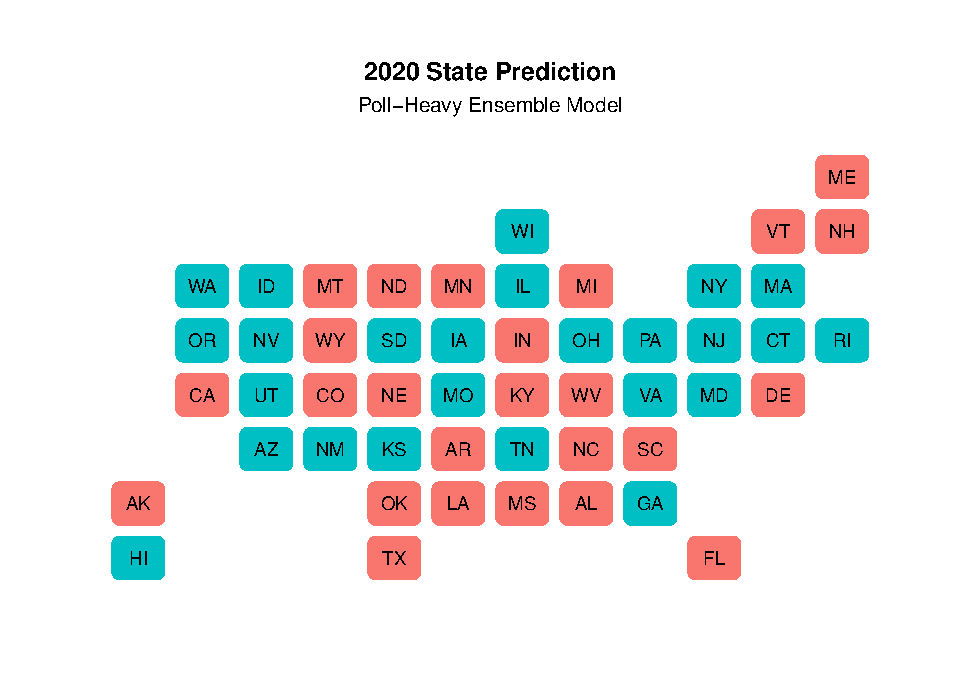
\includegraphics{blog_pred_files/figure-latex/unnamed-chunk-4-1.pdf}

\begin{Shaded}
\begin{Highlighting}[]
\CommentTok{#Predictive Intervals: POLL Ensemble}
\NormalTok{in_sample_poll <-}\StringTok{ }\KeywordTok{predict}\NormalTok{(fit_state_poll, }\DataTypeTok{newdata =}\NormalTok{ new_data_poll, }\DataTypeTok{interval =} \StringTok{"predict"}\NormalTok{) }
\NormalTok{in_sample_demo <-}\StringTok{ }\KeywordTok{predict}\NormalTok{(mod_demog_change, }\DataTypeTok{newdata =}\NormalTok{ real_}\DecValTok{2020}\NormalTok{, }\DataTypeTok{interval =} \StringTok{"predict"}\NormalTok{)}
\NormalTok{in_sample_econ <-}\StringTok{ }\KeywordTok{predict}\NormalTok{(econ_fit, }\DataTypeTok{newdata =}\NormalTok{ new_data_econ, }\DataTypeTok{interval =} \StringTok{"predict"}\NormalTok{)}

\NormalTok{tab1 <-}\StringTok{ }\KeywordTok{as.data.frame}\NormalTok{(}\FloatTok{0.5}\OperatorTok{*}\NormalTok{in_sample_poll }\OperatorTok{+}\StringTok{ }\FloatTok{0.25}\OperatorTok{*}\NormalTok{in_sample_demo }\OperatorTok{+}\StringTok{ }\FloatTok{0.25}\OperatorTok{*}\NormalTok{in_sample_econ) }\OperatorTok
\StringTok{  }\KeywordTok{mutate}\NormalTok{(}\DataTypeTok{state =}\NormalTok{ new_data_poll}\OperatorTok{$}\NormalTok{state) }\OperatorTok
\StringTok{  }\KeywordTok{select}\NormalTok{(state, lwr, fit, upr) }\OperatorTok
\StringTok{  }\KeywordTok{mutate}\NormalTok{(}\DataTypeTok{lwr =} \KeywordTok{round}\NormalTok{(lwr,  }\DataTypeTok{digits =} \DecValTok{2}\NormalTok{)}\OperatorTok{/}\DecValTok{100}\NormalTok{, }
         \DataTypeTok{fit =} \KeywordTok{round}\NormalTok{(fit, }\DataTypeTok{digits =} \DecValTok{2}\NormalTok{)}\OperatorTok{/}\DecValTok{100}\NormalTok{, }
         \DataTypeTok{upr =} \KeywordTok{round}\NormalTok{(upr, }\DataTypeTok{digits =} \DecValTok{2}\NormalTok{)}\OperatorTok{/}\DecValTok{100}\NormalTok{)}\OperatorTok
\StringTok{  }\KeywordTok{mutate}\NormalTok{(}\DataTypeTok{winner =}  \KeywordTok{case_when}\NormalTok{(fit }\OperatorTok{>}\StringTok{ }\FloatTok{.50} \OperatorTok{~}\StringTok{ "Biden"}\NormalTok{,}
\NormalTok{                            fit }\OperatorTok{<}\StringTok{ }\FloatTok{.50} \OperatorTok{~}\StringTok{ "Trump"}\NormalTok{)) }\OperatorTok
\StringTok{  }\KeywordTok{gt}\NormalTok{() }\OperatorTok
\StringTok{   }\KeywordTok{tab_header}\NormalTok{(}\DataTypeTok{title =} \KeywordTok{md}\NormalTok{(}\StringTok{"**Poll-Heavy Ensemble: Projected State Winners and Predictive Intervals for Democratic Vote Share Prediction**"}\NormalTok{), }
               \DataTypeTok{subtitle =} \StringTok{"95% Confidence Intervals"}\NormalTok{) }\OperatorTok
\StringTok{   }\KeywordTok{fmt_percent}\NormalTok{(}\DataTypeTok{columns =} \KeywordTok{c}\NormalTok{(}\StringTok{"lwr"}\NormalTok{, }\StringTok{"fit"}\NormalTok{, }\StringTok{"upr"}\NormalTok{), }\DataTypeTok{decimals =} \DecValTok{1}\NormalTok{) }\OperatorTok
\StringTok{   }\KeywordTok{cols_label}\NormalTok{(}\DataTypeTok{lwr =} \KeywordTok{md}\NormalTok{(}\StringTok{"**Lower Bound**"}\NormalTok{),}
              \DataTypeTok{fit =} \KeywordTok{md}\NormalTok{(}\StringTok{"**Predicted Democratic Vote Share**"}\NormalTok{),}
              \DataTypeTok{upr =} \KeywordTok{md}\NormalTok{(}\StringTok{"**Upper Bound**"}\NormalTok{), }
              \DataTypeTok{state =} \KeywordTok{md}\NormalTok{(}\StringTok{"**State**"}\NormalTok{), }
              \DataTypeTok{winner =} \KeywordTok{md}\NormalTok{(}\StringTok{"**Predicted Winner**"}\NormalTok{)) }\OperatorTok
\StringTok{  }\KeywordTok{tab_source_note}\NormalTok{(}\KeywordTok{md}\NormalTok{(}\StringTok{"*Data: BEA, FiveThirtyEight, World Population Review*"}\NormalTok{)) }







\CommentTok{# diff weights - emphasis on fundamentals}
\NormalTok{ensemble2 <-}\StringTok{ }\FloatTok{0.5}\OperatorTok{*}\NormalTok{econ_pred }\OperatorTok{+}\StringTok{ }\FloatTok{0.25}\OperatorTok{*}\NormalTok{demog_pred }\OperatorTok{+}\StringTok{ }\FloatTok{0.25}\OperatorTok{*}\NormalTok{poll_pred_}\DecValTok{2020}\OperatorTok{$}\NormalTok{pred}
\NormalTok{ensemble_tibble2 <-}\StringTok{ }\KeywordTok{tibble}\NormalTok{(}\DataTypeTok{pred =}\NormalTok{ ensemble2, }\DataTypeTok{state =}\NormalTok{ new_data_poll}\OperatorTok{$}\NormalTok{state)}

\NormalTok{ensemble_tibble2 }\OperatorTok
\StringTok{  }\KeywordTok{mutate}\NormalTok{(}\DataTypeTok{state =}\NormalTok{ state.abb[}\KeywordTok{match}\NormalTok{(state,state.name)]) }\OperatorTok
\StringTok{  }\KeywordTok{select}\NormalTok{(state, pred) }\OperatorTok
\StringTok{  }\KeywordTok{left_join}\NormalTok{(electoral, }\DataTypeTok{by =} \StringTok{"state"}\NormalTok{) }\OperatorTok
\StringTok{  }\KeywordTok{mutate}\NormalTok{(}\DataTypeTok{state_win =} \KeywordTok{case_when}\NormalTok{(pred }\OperatorTok{>}\StringTok{ }\DecValTok{50} \OperatorTok{~}\StringTok{ "Biden"}\NormalTok{,}
\NormalTok{                            pred }\OperatorTok{<}\StringTok{ }\DecValTok{50} \OperatorTok{~}\StringTok{ "Trump"}\NormalTok{)) }\OperatorTok
\StringTok{  }\KeywordTok{group_by}\NormalTok{(state_win) }\OperatorTok
\StringTok{  }\KeywordTok{summarise}\NormalTok{(}\DataTypeTok{electoral_votes =} \KeywordTok{sum}\NormalTok{(}\StringTok{`}\DataTypeTok{2020}\StringTok{`}\NormalTok{)) }\OperatorTok
\StringTok{  }\KeywordTok{gt}\NormalTok{() }\OperatorTok
\StringTok{  }\KeywordTok{tab_header}\NormalTok{(}\DataTypeTok{title =} \KeywordTok{md}\NormalTok{(}\StringTok{"**Fundamentals-Heavy Ensemble: 2020 Electoral Vote Outcome Prediction**"}\NormalTok{), }
               \DataTypeTok{subtitle =} \StringTok{"BIDEN Wins"}\NormalTok{) }\OperatorTok
\StringTok{   }\KeywordTok{cols_label}\NormalTok{(}\DataTypeTok{state_win =} \KeywordTok{md}\NormalTok{(}\StringTok{"**Candidate**"}\NormalTok{),}
               \DataTypeTok{electoral_votes =} \KeywordTok{md}\NormalTok{(}\StringTok{"**Total Electoral Votes**"}\NormalTok{)) }\OperatorTok
\StringTok{  }\KeywordTok{tab_source_note}\NormalTok{(}\KeywordTok{md}\NormalTok{(}\StringTok{"*Data: BEA*"}\NormalTok{))}
\end{Highlighting}
\end{Shaded}

\begin{verbatim}
## `summarise()` ungrouping output (override with `.groups` argument)
\end{verbatim}

\captionsetup[table]{labelformat=empty,skip=1pt}
\begin{longtable}{lr}
\caption*{
\large \textbf{Fundamentals-Heavy Ensemble: 2020 Electoral Vote Outcome Prediction}\\ 
\small BIDEN Wins\\ 
} \\ 
\toprule
\textbf{Candidate} & \textbf{Total Electoral Votes} \\ 
\midrule
Biden & 403 \\ 
Trump & 132 \\ 
\bottomrule
\end{longtable}
\begin{minipage}{\linewidth}
\emph{Data: BEA}\\ 
\end{minipage}

\begin{Shaded}
\begin{Highlighting}[]
\CommentTok{# electoral map table:}
\NormalTok{ensemble_tibble2 }\OperatorTok\StringTok{ }
\StringTok{  }\KeywordTok{mutate}\NormalTok{(}\DataTypeTok{state =} \KeywordTok{as.character}\NormalTok{(state)) }\OperatorTok\StringTok{ }\CommentTok{##`statebins` needs state to be character, not factor!}
\StringTok{  }\KeywordTok{ggplot}\NormalTok{(}\KeywordTok{aes}\NormalTok{(}\DataTypeTok{state =}\NormalTok{ state, }\DataTypeTok{fill =}\NormalTok{ (pred }\OperatorTok{>=}\StringTok{ }\DecValTok{50}\NormalTok{))) }\OperatorTok{+}
\StringTok{  }\KeywordTok{geom_statebins}\NormalTok{() }\OperatorTok{+}
\StringTok{  }\KeywordTok{theme_statebins}\NormalTok{() }\OperatorTok{+}
\StringTok{  }\KeywordTok{labs}\NormalTok{(}\DataTypeTok{title =} \StringTok{"2020 State Prediction"}\NormalTok{,}
       \DataTypeTok{subtitle =} \StringTok{"Fundamentals-Heavy Ensemble Model"}\NormalTok{,}
       \DataTypeTok{fill =} \StringTok{""}\NormalTok{) }\OperatorTok{+}
\StringTok{  }\KeywordTok{theme}\NormalTok{(}\DataTypeTok{legend.position =} \StringTok{"none"}\NormalTok{, }
        \DataTypeTok{plot.subtitle =} \KeywordTok{element_text}\NormalTok{(}\DataTypeTok{size =} \DecValTok{10}\NormalTok{, }\DataTypeTok{hjust =} \FloatTok{0.5}\NormalTok{),}
        \DataTypeTok{plot.title   =} \KeywordTok{element_text}\NormalTok{(}\DataTypeTok{size =} \DecValTok{12}\NormalTok{, }\DataTypeTok{hjust =} \FloatTok{0.5}\NormalTok{, }\DataTypeTok{face =} \StringTok{"bold"}\NormalTok{))}
\end{Highlighting}
\end{Shaded}

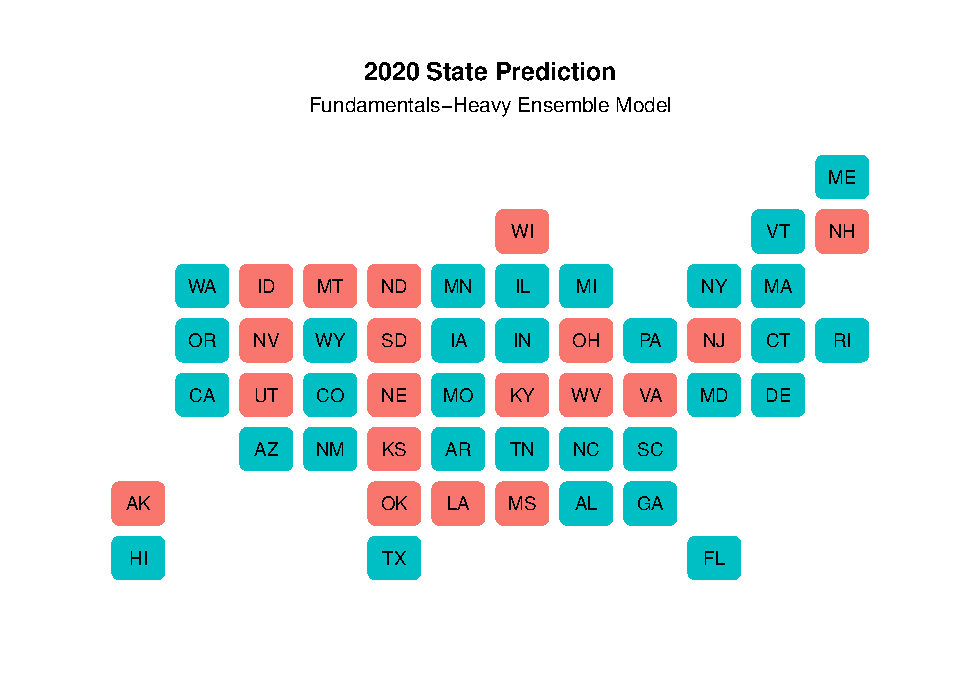
\includegraphics{blog_pred_files/figure-latex/unnamed-chunk-4-2.pdf}

\begin{Shaded}
\begin{Highlighting}[]
\CommentTok{# fundamentals predictive intervals:}
\KeywordTok{as.data.frame}\NormalTok{(}\FloatTok{0.25}\OperatorTok{*}\NormalTok{in_sample_poll }\OperatorTok{+}\StringTok{ }\FloatTok{0.25}\OperatorTok{*}\NormalTok{in_sample_demo }\OperatorTok{+}\StringTok{ }\FloatTok{0.5}\OperatorTok{*}\NormalTok{in_sample_econ) }\OperatorTok
\StringTok{  }\KeywordTok{mutate}\NormalTok{(}\DataTypeTok{state =}\NormalTok{ new_data_poll}\OperatorTok{$}\NormalTok{state) }\OperatorTok
\StringTok{  }\KeywordTok{select}\NormalTok{(state, lwr, fit, upr) }\OperatorTok
\StringTok{  }\KeywordTok{mutate}\NormalTok{(}\DataTypeTok{lwr =} \KeywordTok{round}\NormalTok{(lwr,  }\DataTypeTok{digits =} \DecValTok{2}\NormalTok{)}\OperatorTok{/}\DecValTok{100}\NormalTok{, }
         \DataTypeTok{fit =} \KeywordTok{round}\NormalTok{(fit, }\DataTypeTok{digits =} \DecValTok{2}\NormalTok{)}\OperatorTok{/}\DecValTok{100}\NormalTok{, }
         \DataTypeTok{upr =} \KeywordTok{round}\NormalTok{(upr, }\DataTypeTok{digits =} \DecValTok{2}\NormalTok{)}\OperatorTok{/}\DecValTok{100}\NormalTok{)}\OperatorTok
\StringTok{  }\KeywordTok{mutate}\NormalTok{(}\DataTypeTok{winner =}  \KeywordTok{case_when}\NormalTok{(fit }\OperatorTok{>}\StringTok{ }\FloatTok{.50} \OperatorTok{~}\StringTok{ "Biden"}\NormalTok{,}
\NormalTok{                            fit }\OperatorTok{<}\StringTok{ }\FloatTok{.50} \OperatorTok{~}\StringTok{ "Trump"}\NormalTok{)) }\OperatorTok
\StringTok{  }\KeywordTok{gt}\NormalTok{() }\OperatorTok
\StringTok{   }\KeywordTok{tab_header}\NormalTok{(}\DataTypeTok{title =} \KeywordTok{md}\NormalTok{(}\StringTok{"**Fundamentals-Heavy Ensemble: Projected State Winners and Predictive Intervals for Democratic Vote Share Prediction**"}\NormalTok{), }
               \DataTypeTok{subtitle =} \StringTok{"95% Confidence Intervals"}\NormalTok{) }\OperatorTok
\StringTok{   }\KeywordTok{fmt_percent}\NormalTok{(}\DataTypeTok{columns =} \KeywordTok{c}\NormalTok{(}\StringTok{"lwr"}\NormalTok{, }\StringTok{"fit"}\NormalTok{, }\StringTok{"upr"}\NormalTok{), }\DataTypeTok{decimals =} \DecValTok{1}\NormalTok{) }\OperatorTok
\StringTok{   }\KeywordTok{cols_label}\NormalTok{(}\DataTypeTok{lwr =} \KeywordTok{md}\NormalTok{(}\StringTok{"**Lower Bound**"}\NormalTok{),}
              \DataTypeTok{fit =} \KeywordTok{md}\NormalTok{(}\StringTok{"**Predicted Democratic Vote Share**"}\NormalTok{),}
              \DataTypeTok{upr =} \KeywordTok{md}\NormalTok{(}\StringTok{"**Upper Bound**"}\NormalTok{), }
              \DataTypeTok{state =} \KeywordTok{md}\NormalTok{(}\StringTok{"**State**"}\NormalTok{), }
              \DataTypeTok{winner =} \KeywordTok{md}\NormalTok{(}\StringTok{"**Predicted Winner**"}\NormalTok{)) }\OperatorTok
\StringTok{  }\KeywordTok{tab_source_note}\NormalTok{(}\KeywordTok{md}\NormalTok{(}\StringTok{"*Data: BEA, FiveThirtyEight, World Population Review*"}\NormalTok{))}
\end{Highlighting}
\end{Shaded}

\captionsetup[table]{labelformat=empty,skip=1pt}
\begin{longtable}{lrrrl}
\caption*{
\large \textbf{Fundamentals-Heavy Ensemble: Projected State Winners and Predictive Intervals for Democratic Vote Share Prediction}\\ 
\small 95\% Confidence Intervals\\ 
} \\ 
\toprule
\textbf{State} & \textbf{Lower Bound} & \textbf{Predicted Democratic Vote Share} & \textbf{Upper Bound} & \textbf{Predicted Winner} \\ 
\midrule
Alabama & $45.7\%$ & $54.2\%$ & $62.6\%$ & Biden \\ 
Alaska & $35.3\%$ & $43.9\%$ & $52.5\%$ & Trump \\ 
Arizona & $51.1\%$ & $59.8\%$ & $68.4\%$ & Biden \\ 
Arkansas & $41.6\%$ & $50.1\%$ & $58.6\%$ & Biden \\ 
California & $53.4\%$ & $62.2\%$ & $71.0\%$ & Biden \\ 
Colorado & $46.4\%$ & $54.9\%$ & $63.4\%$ & Biden \\ 
Connecticut & $48.0\%$ & $56.5\%$ & $65.0\%$ & Biden \\ 
Delaware & $51.1\%$ & $59.5\%$ & $67.8\%$ & Biden \\ 
Florida & $42.8\%$ & $51.4\%$ & $60.0\%$ & Biden \\ 
Georgia & $46.9\%$ & $55.6\%$ & $64.3\%$ & Biden \\ 
Hawaii & $54.0\%$ & $70.5\%$ & $87.0\%$ & Biden \\ 
Idaho & $37.0\%$ & $45.6\%$ & $54.2\%$ & Trump \\ 
Illinois & $47.9\%$ & $56.4\%$ & $64.8\%$ & Biden \\ 
Indiana & $43.5\%$ & $52.1\%$ & $60.7\%$ & Biden \\ 
Iowa & $50.3\%$ & $58.8\%$ & $67.3\%$ & Biden \\ 
Kansas & $40.2\%$ & $48.6\%$ & $57.0\%$ & Trump \\ 
Kentucky & $41.3\%$ & $49.9\%$ & $58.4\%$ & Trump \\ 
Louisiana & $39.1\%$ & $47.6\%$ & $56.1\%$ & Trump \\ 
Maine & $45.2\%$ & $53.6\%$ & $62.0\%$ & Biden \\ 
Maryland & $45.3\%$ & $54.1\%$ & $62.9\%$ & Biden \\ 
Massachusetts & $52.8\%$ & $61.3\%$ & $69.8\%$ & Biden \\ 
Michigan & $44.6\%$ & $53.2\%$ & $61.8\%$ & Biden \\ 
Minnesota & $50.4\%$ & $59.0\%$ & $67.6\%$ & Biden \\ 
Mississippi & $37.8\%$ & $46.2\%$ & $54.7\%$ & Trump \\ 
Missouri & $45.9\%$ & $54.4\%$ & $62.8\%$ & Biden \\ 
Montana & $38.7\%$ & $47.3\%$ & $55.9\%$ & Trump \\ 
Nebraska & $34.1\%$ & $42.6\%$ & $51.2\%$ & Trump \\ 
Nevada & $36.9\%$ & $45.4\%$ & $53.8\%$ & Trump \\ 
New Hampshire & $40.0\%$ & $48.5\%$ & $56.9\%$ & Trump \\ 
New Jersey & $37.9\%$ & $46.2\%$ & $54.6\%$ & Trump \\ 
New Mexico & $46.5\%$ & $55.0\%$ & $63.5\%$ & Biden \\ 
New York & $45.7\%$ & $54.1\%$ & $62.5\%$ & Biden \\ 
North Carolina & $45.0\%$ & $53.7\%$ & $62.4\%$ & Biden \\ 
North Dakota & $32.3\%$ & $40.6\%$ & $49.0\%$ & Trump \\ 
Ohio & $39.3\%$ & $47.7\%$ & $56.1\%$ & Trump \\ 
Oklahoma & $34.1\%$ & $42.7\%$ & $51.3\%$ & Trump \\ 
Oregon & $48.0\%$ & $56.3\%$ & $64.6\%$ & Biden \\ 
Pennsylvania & $54.3\%$ & $63.2\%$ & $72.0\%$ & Biden \\ 
Rhode Island & $42.1\%$ & $50.5\%$ & $58.9\%$ & Biden \\ 
South Carolina & $44.0\%$ & $52.8\%$ & $61.5\%$ & Biden \\ 
South Dakota & $35.1\%$ & $43.5\%$ & $51.8\%$ & Trump \\ 
Tennessee & $45.0\%$ & $53.6\%$ & $62.1\%$ & Biden \\ 
Texas & $45.1\%$ & $53.7\%$ & $62.3\%$ & Biden \\ 
Utah & $30.9\%$ & $39.3\%$ & $47.6\%$ & Trump \\ 
Vermont & $57.6\%$ & $66.2\%$ & $75.0\%$ & Biden \\ 
Virginia & $38.0\%$ & $46.3\%$ & $54.5\%$ & Trump \\ 
Washington & $42.2\%$ & $50.9\%$ & $59.6\%$ & Biden \\ 
West Virginia & $36.3\%$ & $44.6\%$ & $52.9\%$ & Trump \\ 
Wisconsin & $34.5\%$ & $42.7\%$ & $50.9\%$ & Trump \\ 
Wyoming & $44.0\%$ & $52.9\%$ & $61.8\%$ & Biden \\ 
\bottomrule
\end{longtable}
\begin{minipage}{\linewidth}
\emph{Data: BEA, FiveThirtyEight, World Population Review}\\ 
\end{minipage}

\begin{itemize}
\tightlist
\item
  difference when weighing fundamentals (econ and incumbency) versus
  polls:

  \begin{itemize}
  \tightlist
  \item
    Ohio, Virginia, North Carolina RED with poll-heavy
  \end{itemize}
\end{itemize}

\hypertarget{checking-fit-can-you-even-do-this-if-its-different-years-and-there-are-some-nas}{%
\section{CHECKING FIT : can you even do this if it's different years and
there are some
NAs?}\label{checking-fit-can-you-even-do-this-if-its-different-years-and-there-are-some-nas}}

\hypertarget{in-sample}{%
\subsection{In Sample}\label{in-sample}}

\begin{Shaded}
\begin{Highlighting}[]
\KeywordTok{summary}\NormalTok{(dat)}
\KeywordTok{summary}\NormalTok{(dat_change)}
\KeywordTok{summary}\NormalTok{(q3_econ)}

\CommentTok{# predictions}

\CommentTok{# R-square is: 0.936}


\CommentTok{# ALTERNATIVE MODEL PREDICTION}

\NormalTok{df_poll2 <-}\StringTok{ }\NormalTok{dat }\OperatorTok
\StringTok{  }\KeywordTok{select}\NormalTok{(state, year, avg_poll)}\OperatorTok\StringTok{ }
\StringTok{  }\KeywordTok{add_predictions}\NormalTok{(fit_state_poll) }\OperatorTok
\StringTok{  }\KeywordTok{mutate}\NormalTok{(}\DataTypeTok{state =}\NormalTok{ state.abb[}\KeywordTok{match}\NormalTok{(state,state.name)])}\OperatorTok
\StringTok{  }\KeywordTok{mutate}\NormalTok{(}\DataTypeTok{pollpred =} \FloatTok{0.25}\OperatorTok{*}\NormalTok{pred)}
\NormalTok{df_demo2 <-}\StringTok{ }\NormalTok{dat_change }\OperatorTok
\StringTok{  }\KeywordTok{select}\NormalTok{(state, year, Black_change, Hispanic_change, Asian_change)}\OperatorTok\StringTok{ }
\StringTok{  }\KeywordTok{add_predictions}\NormalTok{(mod_demog_change) }\OperatorTok
\StringTok{  }\KeywordTok{mutate}\NormalTok{(}\DataTypeTok{demopred =} \FloatTok{0.25}\OperatorTok{*}\NormalTok{pred)}
\NormalTok{df_econ2 <-}\StringTok{ }\NormalTok{q3_econ }\OperatorTok
\StringTok{  }\KeywordTok{select}\NormalTok{(state, year, gdp_growth, incumbent)}\OperatorTok\StringTok{ }
\StringTok{  }\KeywordTok{add_predictions}\NormalTok{(econ_fit) }\OperatorTok
\StringTok{  }\KeywordTok{mutate}\NormalTok{(}\DataTypeTok{econpred =} \FloatTok{0.5}\OperatorTok{*}\NormalTok{pred)}

\NormalTok{resid2 <-}\StringTok{ }\NormalTok{df_demo2}\OperatorTok
\KeywordTok{left_join}\NormalTok{(df_poll2, }\DataTypeTok{by =} \KeywordTok{c}\NormalTok{(}\StringTok{"state"}\NormalTok{, }\StringTok{"year"}\NormalTok{)) }\OperatorTok
\KeywordTok{left_join}\NormalTok{(df_econ2, }\DataTypeTok{by =} \KeywordTok{c}\NormalTok{(}\StringTok{"state"}\NormalTok{, }\StringTok{"year"}\NormalTok{)) }\OperatorTok
\KeywordTok{mutate}\NormalTok{(}\DataTypeTok{weighted_pred =}\NormalTok{ pollpred }\OperatorTok{+}\StringTok{ }\NormalTok{demopred }\OperatorTok{+}\StringTok{ }\NormalTok{econpred) }\OperatorTok
\KeywordTok{select}\NormalTok{(state, year, weighted_pred) }\OperatorTok
\KeywordTok{left_join}\NormalTok{(pvstate_df, }\KeywordTok{c}\NormalTok{(}\StringTok{"state"}\NormalTok{, }\StringTok{"year"}\NormalTok{)) }\OperatorTok
\KeywordTok{mutate}\NormalTok{(}\DataTypeTok{residual =}\NormalTok{ D_pv2p }\OperatorTok{-}\StringTok{ }\NormalTok{weighted_pred) }\OperatorTok
\KeywordTok{select}\NormalTok{(state, year, weighted_pred, D_pv2p, residual) }\OperatorTok
\KeywordTok{mutate}\NormalTok{(}\DataTypeTok{numerator =}\NormalTok{ residual}\OperatorTok{^}\DecValTok{2}\NormalTok{,}
       \DataTypeTok{denominator =}\NormalTok{ (D_pv2p }\OperatorTok{-}\StringTok{ }\KeywordTok{mean}\NormalTok{(resid}\OperatorTok{$}\NormalTok{D_pv2p, }\DataTypeTok{na.rm =} \OtherTok{TRUE}\NormalTok{))}\OperatorTok{^}\DecValTok{2}\NormalTok{) }\OperatorTok
\StringTok{  }\KeywordTok{filter}\NormalTok{(year }\OperatorTok{>=}\StringTok{ }\DecValTok{2008}\NormalTok{)}

\DecValTok{1}\OperatorTok{-}\StringTok{ }\NormalTok{(}\KeywordTok{sum}\NormalTok{(resid2}\OperatorTok{$}\NormalTok{numerator, }\DataTypeTok{na.rm =} \OtherTok{TRUE}\NormalTok{)}\OperatorTok{/}\KeywordTok{sum}\NormalTok{(resid2}\OperatorTok{$}\NormalTok{denominator, }\DataTypeTok{na.rm =} \OtherTok{TRUE}\NormalTok{))}

\CommentTok{# R squared is 0.926}
\end{Highlighting}
\end{Shaded}

Model elements: fit\_state\_poll: original poll model uses dat
pred\_2020: poll prediction uses new\_data\_poll mod\_demog\_change:
original demo model uses dat\_change demog\_pred: demography model
prediction uses real\_2020

You simply have to (1) subset out the data to leave one observation out
(ex. 2016) when you estimate the regression coefficients of each model,
(2) run regression and estimate the coefficients for each model, (3) do
the prediction using each model with the left out data (ex. 2016) as
newdata, (4) do ensemble of that prediction, and (5) compare it with the
true value for ex. 2016.

\hypertarget{out-of-sample-can-you-even-do-this-if-its-different-years}{%
\subsection{Out of Sample -- can you even do this if it's different
years????}\label{out-of-sample-can-you-even-do-this-if-its-different-years}}

\begin{Shaded}
\begin{Highlighting}[]
\NormalTok{true <-}\StringTok{ }\NormalTok{dat_change }\OperatorTok
\StringTok{  }\KeywordTok{left_join}\NormalTok{(df_econ, }\DataTypeTok{by =} \KeywordTok{c}\NormalTok{(}\StringTok{"state"}\NormalTok{, }\StringTok{"year"}\NormalTok{)) }\OperatorTok
\StringTok{  }\KeywordTok{filter}\NormalTok{(year }\OperatorTok{==}\StringTok{ }\DecValTok{2016}\NormalTok{) }\OperatorTok
\StringTok{  }\KeywordTok{select}\NormalTok{(year, state, D_pv2p) }\OperatorTok
\StringTok{  }\KeywordTok{distinct}\NormalTok{() }\OperatorTok
\StringTok{  }\KeywordTok{na.omit}\NormalTok{()}


\NormalTok{d <-}\StringTok{ }\NormalTok{dat_change[}\OperatorTok{!}\NormalTok{(dat_change}\OperatorTok{$}\NormalTok{Asian_change }\OperatorTok{==}\StringTok{ }\FloatTok{0.0000000}\NormalTok{),] }\OperatorTok
\StringTok{  }\KeywordTok{na.omit}\NormalTok{()}

\NormalTok{all_years <-}\StringTok{ }\KeywordTok{seq}\NormalTok{(}\DataTypeTok{from=}\DecValTok{1998}\NormalTok{, }\DataTypeTok{to=}\DecValTok{2016}\NormalTok{, }\DataTypeTok{by=}\DecValTok{4}\NormalTok{)}
\NormalTok{outsamp_dflist <-}\StringTok{ }\KeywordTok{lapply}\NormalTok{(all_years, }\ControlFlowTok{function}\NormalTok{(year)\{}
 
\NormalTok{  true_inc <-}\StringTok{ }\NormalTok{true }\OperatorTok
\StringTok{    }\KeywordTok{filter}\NormalTok{(state }\OperatorTok{==}\StringTok{ "FL"}\NormalTok{)}

  \CommentTok{##fundamental model out-of-sample prediction}
\NormalTok{  fit_out_poll <-}\StringTok{ }\KeywordTok{lm}\NormalTok{(D_pv2p }\OperatorTok{~}\StringTok{ }\NormalTok{avg_poll }\OperatorTok{+}\StringTok{ }\KeywordTok{as.factor}\NormalTok{(state), }\DataTypeTok{data =}\NormalTok{ dat[dat}\OperatorTok{$}\NormalTok{year }\OperatorTok{!=}\StringTok{ }\DecValTok{2004}\NormalTok{,])}
\NormalTok{  fit_out_demo <-}\StringTok{ }\KeywordTok{lm}\NormalTok{(D_pv2p }\OperatorTok{~}\StringTok{ }\NormalTok{Black_change }\OperatorTok{+}\StringTok{ }\NormalTok{Hispanic_change }\OperatorTok{+}\StringTok{ }\NormalTok{Asian_change }\OperatorTok{+}
\StringTok{                         }\KeywordTok{as.factor}\NormalTok{(state), }\DataTypeTok{data =}\NormalTok{ d[d}\OperatorTok{$}\NormalTok{year }\OperatorTok{!=}\StringTok{ }\DecValTok{2004}\NormalTok{,])}
\NormalTok{  fit_out_econ <-}\StringTok{ }\KeywordTok{lm}\NormalTok{(D_pv2p }\OperatorTok{~}\StringTok{ }\NormalTok{gdp_growth}\OperatorTok{*}\NormalTok{incumbent }\OperatorTok{+}\StringTok{ }\KeywordTok{as.factor}\NormalTok{(state), }\DataTypeTok{data =}\NormalTok{ q3_econ[q3_econ}\OperatorTok{$}\NormalTok{year }\OperatorTok{!=}\StringTok{ }\DecValTok{2004}\NormalTok{,])}

\NormalTok{  mod_poll <-}\StringTok{ }\FloatTok{0.5}\OperatorTok{*}\StringTok{ }\KeywordTok{mean}\NormalTok{(}\KeywordTok{predict}\NormalTok{(fit_out_poll, dat[dat}\OperatorTok{$}\NormalTok{year }\OperatorTok{==}\StringTok{ }\DecValTok{2004} \OperatorTok{&}\StringTok{ }\NormalTok{dat}\OperatorTok{$}\NormalTok{state }\OperatorTok{==}\StringTok{ "FL"}\NormalTok{,]), }\DataTypeTok{na.rm =} \OtherTok{TRUE}\NormalTok{)}
\NormalTok{  mod_demog <-}\StringTok{ }\FloatTok{0.25}\OperatorTok{*}\KeywordTok{predict}\NormalTok{(fit_out_demo, d[d}\OperatorTok{$}\NormalTok{year }\OperatorTok{==}\StringTok{ }\DecValTok{2004} \OperatorTok{&}\StringTok{ }\NormalTok{d}\OperatorTok{$}\NormalTok{state }\OperatorTok{==}\StringTok{ "FL"}\NormalTok{,])}
\NormalTok{  mod_econ <-}\StringTok{ }\FloatTok{0.25}\OperatorTok{*}\KeywordTok{predict}\NormalTok{(fit_out_econ, q3_econ[q3_econ}\OperatorTok{$}\NormalTok{year }\OperatorTok{==}\StringTok{ }\DecValTok{2004} \OperatorTok{&}\StringTok{ }\NormalTok{q3_econ}\OperatorTok{$}\NormalTok{state }\OperatorTok{==}\StringTok{ "FL"}\NormalTok{,])}
  
\NormalTok{  mod <-}\StringTok{ }\NormalTok{mod_poll }\OperatorTok{+}\StringTok{ }\NormalTok{mod_demog }\OperatorTok{+}\StringTok{ }\NormalTok{mod_econ}
  

\NormalTok{  fl_margin_error =}\StringTok{ }\NormalTok{mod }\OperatorTok{-}\StringTok{ }\NormalTok{true_inc}\OperatorTok{$}\NormalTok{D_pv2p}
        
        
       
        \KeywordTok{cbind}\NormalTok{(}\DataTypeTok{poll_winner_correct =}\NormalTok{ (mod_poll }\OperatorTok{>}\StringTok{ }\DecValTok{50}\NormalTok{) }\OperatorTok{==}\StringTok{ }\NormalTok{(true_inc}\OperatorTok{$}\NormalTok{D_pv2p }\OperatorTok{>}\StringTok{ }\DecValTok{50}\NormalTok{),}
        \DataTypeTok{demo_winner_correct =}\NormalTok{ (mod_demog }\OperatorTok{>}\StringTok{ }\DecValTok{50}\NormalTok{) }\OperatorTok{==}\StringTok{ }\NormalTok{(true_inc}\OperatorTok{$}\NormalTok{D_pv2p }\OperatorTok{>}\StringTok{ }\DecValTok{50}\NormalTok{),}
        \DataTypeTok{econ_winner_correct =}\NormalTok{ (mod_econ }\OperatorTok{>}\StringTok{ }\DecValTok{50}\NormalTok{) }\OperatorTok{==}\StringTok{ }\NormalTok{(true_inc}\OperatorTok{$}\NormalTok{D_pv2p }\OperatorTok{>}\StringTok{ }\DecValTok{50}\NormalTok{))}
  
\NormalTok{\})}




\KeywordTok{sum}\NormalTok{(poll_margin_error, demo_margin_error, econ_margin_error, }\DataTypeTok{na.rm =}\NormalTok{ T)}


\NormalTok{outsamp_df <-}\StringTok{ }\KeywordTok{do.call}\NormalTok{(rbind, outsamp_dflist) }\CommentTok{#}
\KeywordTok{colMeans}\NormalTok{(}\KeywordTok{abs}\NormalTok{(outsamp_df[}\DecValTok{2}\OperatorTok{:}\DecValTok{4}\NormalTok{]), }\DataTypeTok{na.rm=}\NormalTok{T) }\CommentTok{#}
\KeywordTok{colMeans}\NormalTok{(outsamp_df[}\DecValTok{5}\OperatorTok{:}\DecValTok{7}\NormalTok{], }\DataTypeTok{na.rm=}\NormalTok{T) }\CommentTok{### classification accuracy}

\NormalTok{outsamp_df[,}\KeywordTok{c}\NormalTok{(}\StringTok{"year"}\NormalTok{,}\StringTok{"econ_winner_correct"}\NormalTok{,}\StringTok{"poll_winner_correct"}\NormalTok{,}\StringTok{"plus_winner_correct"}\NormalTok{)] }\CommentTok{#}
\end{Highlighting}
\end{Shaded}

\begin{Shaded}
\begin{Highlighting}[]
\KeywordTok{summary}\NormalTok{(dat)}
\KeywordTok{summary}\NormalTok{(dat_change)}
\KeywordTok{summary}\NormalTok{(q3_econ)}

\CommentTok{# took 2016 out of the data: }
\NormalTok{out_poll <-}\StringTok{ }\NormalTok{dat }\OperatorTok
\StringTok{  }\KeywordTok{filter}\NormalTok{(year }\OperatorTok{!=}\StringTok{ }\DecValTok{2016}\NormalTok{)}
\NormalTok{out_demo <-}\StringTok{ }\NormalTok{dat_change }\OperatorTok
\StringTok{  }\KeywordTok{filter}\NormalTok{(year }\OperatorTok{!=}\StringTok{ }\DecValTok{2016}\NormalTok{)}
\NormalTok{out_econ <-}\StringTok{ }\NormalTok{q3_econ }\OperatorTok
\StringTok{  }\KeywordTok{filter}\NormalTok{(year }\OperatorTok{!=}\StringTok{ }\DecValTok{2016}\NormalTok{)}

\CommentTok{# running regressions without 2016: }
\NormalTok{fit_out_poll <-}\StringTok{ }\KeywordTok{lm}\NormalTok{(D_pv2p }\OperatorTok{~}\StringTok{ }\NormalTok{avg_poll }\OperatorTok{+}\StringTok{ }\KeywordTok{as.factor}\NormalTok{(state), }\DataTypeTok{data =}\NormalTok{ out_poll)}
\NormalTok{fit_out_demo <-}\StringTok{ }\KeywordTok{lm}\NormalTok{(D_pv2p }\OperatorTok{~}\StringTok{ }\NormalTok{Black_change }\OperatorTok{+}\StringTok{ }\NormalTok{Hispanic_change }\OperatorTok{+}\StringTok{ }\NormalTok{Asian_change }\OperatorTok{+}
\StringTok{                         }\KeywordTok{as.factor}\NormalTok{(state), }\DataTypeTok{data =}\NormalTok{ out_demo)}
\NormalTok{fit_out_econ <-}\StringTok{ }\KeywordTok{lm}\NormalTok{(D_pv2p }\OperatorTok{~}\StringTok{ }\NormalTok{gdp_growth}\OperatorTok{*}\NormalTok{incumbent }\OperatorTok{+}\StringTok{ }\KeywordTok{as.factor}\NormalTok{(state), }\DataTypeTok{data =}\NormalTok{ out_econ)}

\CommentTok{# predict without 2016}
\KeywordTok{predict}\NormalTok{(fit_out_poll, }\DataTypeTok{newdata =}\NormalTok{ out_poll)}
\KeywordTok{predict}\NormalTok{(fit_out_demo, }\DataTypeTok{newdata =}\NormalTok{ out_demo)}
\KeywordTok{predict}\NormalTok{(fit_out_econ, }\DataTypeTok{newdata =}\NormalTok{ out_econ)}







\NormalTok{outsamp_errors <-}\StringTok{ }\KeywordTok{sapply}\NormalTok{(}\DecValTok{1}\OperatorTok{:}\DecValTok{1000}\NormalTok{, }\ControlFlowTok{function}\NormalTok{(i)\{}
\NormalTok{years_outsamp <-}\StringTok{ }\KeywordTok{sample}\NormalTok{(tfc_df}\OperatorTok{$}\NormalTok{year, }\DecValTok{8}\NormalTok{)}
\NormalTok{outsamp_mod <-}\StringTok{ }\KeywordTok{lm}\NormalTok{(pv2p }\OperatorTok{~}\StringTok{ }\NormalTok{GDP_growth_qt }\OperatorTok{+}\StringTok{ }\NormalTok{net_approve }\OperatorTok{+}\StringTok{ }\NormalTok{incumbent, tfc_df[}\OperatorTok{!}\NormalTok{(tfc_df}\OperatorTok{$}\NormalTok{year }\OperatorTok\StringTok{ }\NormalTok{years_outsamp),])}
\NormalTok{outsamp_pred <-}\StringTok{ }\KeywordTok{predict}\NormalTok{(outsamp_mod, }
                        \DataTypeTok{newdata =}\NormalTok{ tfc_df[tfc_df}\OperatorTok{$}\NormalTok{year }\OperatorTok\StringTok{ }\NormalTok{years_outsamp,])}
\NormalTok{outsamp_true <-}\StringTok{ }\NormalTok{tfc_df}\OperatorTok{$}\NormalTok{pv2p[tfc_df}\OperatorTok{$}\NormalTok{year }\OperatorTok\StringTok{ }\NormalTok{years_outsamp]}
\KeywordTok{mean}\NormalTok{(outsamp_pred }\OperatorTok{-}\StringTok{ }\NormalTok{outsamp_true)}
\NormalTok{\})}

\CommentTok{# visualize in histogram}
\KeywordTok{hist}\NormalTok{(outsamp_errors,}
     \DataTypeTok{xlab =} \StringTok{"Out-of-Sample Residual"}\NormalTok{,}
     \DataTypeTok{main =} \StringTok{"Time-for-Change Model: }\CharTok{\textbackslash{}n}\StringTok{ Mean Out-of-Sample Residual (1000 Runs)"}\NormalTok{,}
     \DataTypeTok{xlim =} \KeywordTok{c}\NormalTok{(}\OperatorTok{-}\DecValTok{15}\NormalTok{, }\DecValTok{15}\NormalTok{), }
     \DataTypeTok{ylim =} \KeywordTok{c}\NormalTok{(}\DecValTok{0}\NormalTok{, }\DecValTok{270}\NormalTok{))}

\CommentTok{# quantify by taking the means of the outsample errors }
\KeywordTok{mean}\NormalTok{(}\KeywordTok{abs}\NormalTok{(outsamp_errors))}















\NormalTok{outsamp_errors <-}\StringTok{ }\KeywordTok{sapply}\NormalTok{(}\DecValTok{1}\OperatorTok{:}\DecValTok{1000}\NormalTok{, }\ControlFlowTok{function}\NormalTok{(i)\{}
  \CommentTok{# years to omit}
\NormalTok{years_outsamp <-}\StringTok{ }\KeywordTok{seq}\NormalTok{(}\DataTypeTok{from=}\DecValTok{2008}\NormalTok{, }\DataTypeTok{to=}\DecValTok{2016}\NormalTok{, }\DataTypeTok{by=}\DecValTok{4}\NormalTok{)}
\NormalTok{omit_data <-}\StringTok{ }\NormalTok{data[}\OperatorTok{!}\NormalTok{(data}\OperatorTok{$}\NormalTok{year }\OperatorTok\StringTok{ }\NormalTok{years_outsamp),]}

\CommentTok{# outsample years in each model}
\NormalTok{outsamp_mod_poll <-}\StringTok{ }\KeywordTok{lm}\NormalTok{(D_pv2p }\OperatorTok{~}\StringTok{ }\NormalTok{avg_poll }\OperatorTok{+}\StringTok{ }\KeywordTok{as.factor}\NormalTok{(state), omit_data)}
\NormalTok{outsamp_mod_demog <-}\StringTok{ }\KeywordTok{lm}\NormalTok{(D_pv2p }\OperatorTok{~}\StringTok{ }\NormalTok{Black_change }\OperatorTok{+}\StringTok{ }\NormalTok{Hispanic_change }\OperatorTok{+}\StringTok{ }\NormalTok{Asian_change }\OperatorTok{+}\StringTok{ }
\StringTok{    }\KeywordTok{as.factor}\NormalTok{(state), omit_data)}
\NormalTok{outsamp_mod_econ <-}\StringTok{ }\KeywordTok{lm}\NormalTok{(D_pv2p }\OperatorTok{~}\StringTok{ }\NormalTok{gdp_growth }\OperatorTok{+}\StringTok{ }\NormalTok{incumbent, omit_data)}

\CommentTok{# draw predictions from each model}
\NormalTok{outsamp_pred_poll <-}\StringTok{ }\NormalTok{omit_data }\OperatorTok
\StringTok{  }\KeywordTok{select}\NormalTok{(state, year, avg_poll)}\OperatorTok\StringTok{ }
\StringTok{  }\KeywordTok{add_predictions}\NormalTok{(outsamp_mod_poll)}\OperatorTok
\StringTok{  }\KeywordTok{mutate}\NormalTok{(}\DataTypeTok{pollpred =} \FloatTok{0.5}\OperatorTok{*}\NormalTok{pred)}
\NormalTok{outsamp_pred_demog <-}\StringTok{ }\NormalTok{omit_data }\OperatorTok
\StringTok{  }\KeywordTok{select}\NormalTok{(state, year, Black_change, Hispanic_change, Asian_change)}\OperatorTok\StringTok{ }
\StringTok{  }\KeywordTok{add_predictions}\NormalTok{(outsamp_mod_demog) }\OperatorTok
\StringTok{  }\KeywordTok{mutate}\NormalTok{(}\DataTypeTok{demopred =} \FloatTok{0.25}\OperatorTok{*}\NormalTok{pred)}
\NormalTok{outsamp_pred_econ <-}\StringTok{ }\NormalTok{omit_data }\OperatorTok
\StringTok{  }\KeywordTok{select}\NormalTok{(state, year, gdp_growth, incumbent)}\OperatorTok\StringTok{ }
\StringTok{  }\KeywordTok{add_predictions}\NormalTok{(outsamp_mod_econ) }\OperatorTok
\StringTok{  }\KeywordTok{mutate}\NormalTok{(}\DataTypeTok{econpred =} \FloatTok{0.25}\OperatorTok{*}\NormalTok{pred)}


\NormalTok{outsamp_pred <-}\StringTok{ }\FloatTok{0.5}\OperatorTok{*}\NormalTok{outsamp_pred_poll}\OperatorTok{$}\NormalTok{pollpred }\OperatorTok{+}\StringTok{ }\FloatTok{0.25}\OperatorTok{*}\NormalTok{outsamp_pred_demog}\OperatorTok{$}\NormalTok{demopred }\OperatorTok{+}\StringTok{ }\FloatTok{0.25}\OperatorTok{*}\NormalTok{outsamp_pred_econ}\OperatorTok{$}\NormalTok{econpred}

\CommentTok{# extract true value}
\NormalTok{outsamp_true <-}\StringTok{ }\NormalTok{omit_data}\OperatorTok{$}\NormalTok{D_pv2p[omit_data}\OperatorTok{$}\NormalTok{year }\OperatorTok\StringTok{ }\NormalTok{years_outsamp]}

\KeywordTok{mean}\NormalTok{(outsamp_pred }\OperatorTok{-}\StringTok{ }\NormalTok{outsamp_true, }\DataTypeTok{na.rm =} \OtherTok{TRUE}\NormalTok{)}
\NormalTok{\})}
\end{Highlighting}
\end{Shaded}

\hypertarget{weighted-ensemble}{%
\section{Weighted Ensemble}\label{weighted-ensemble}}

\begin{itemize}
\tightlist
\item
  I am placing the most weight on polls,
\item
  have as.factor state for each poll
\end{itemize}

in sample fit: .5(poll)+.25(econ)+.25(demo) true value -
(.5(poll)+.25(econ)+.25(demo)) 0.5predict() + 0.25predict() +
.25predict()

out of sample fit: - exclude 2016 and then do whole process and do
regression parameter without 2016 - predict with ensemble fit (without
2016) and make new data = 2016 data\\
- make sure new data has a column named state and states listed

There should be a column named ``state'' And ex. PA? Then your new data
should have ``state'' column with ``PA'' in that column True value -
(0.5x51 + 0.25x49 + 0.25x50)

you could do ensemble at the electoral college level (0.5x400 + 0.25x390
+ 0.25x380)

\hypertarget{modified-time-for-change}{%
\section{Modified Time-For-Change}\label{modified-time-for-change}}

\begin{itemize}
\tightlist
\item
  economic approval rating
\item
  state AND national approval
\item
  GDP/RDI Growth
\item
  Incumbency
\item
  Jobs
\item
  2020 demographics
\item
  predict national pop\_vote
\end{itemize}

polls model and demographic will have popular vote share from state

\begin{itemize}
\tightlist
\item
  state poll, demo, AND economic model
\item
  maybe add incumbency indicator to either poll or economy

  \begin{itemize}
  \tightlist
  \item
    find link on slack
  \end{itemize}
\end{itemize}

\hypertarget{does-this-ensemble-even-work-if-there-are-tons-of-nas-in-some-predictions-and-none-in-others}{%
\section{DOES THIS ENSEMBLE EVEN WORK IF THERE ARE TONS OF NAs in some
predictions and none in
others?}\label{does-this-ensemble-even-work-if-there-are-tons-of-nas-in-some-predictions-and-none-in-others}}

\begin{Shaded}
\begin{Highlighting}[]
\NormalTok{pop <-}\StringTok{ }\NormalTok{popvote_df }\OperatorTok
\StringTok{  }\KeywordTok{select}\NormalTok{(year, party, incumbent)}

\KeywordTok{summary}\NormalTok{(dat)}

\NormalTok{poll_demo_model <-}\StringTok{ }\NormalTok{dat }\OperatorTok
\StringTok{  }\KeywordTok{left_join}\NormalTok{(dat_change, }\DataTypeTok{by =} \KeywordTok{c}\NormalTok{(}\StringTok{"year"}\NormalTok{, }\StringTok{"state"}\NormalTok{)) }\OperatorTok
\StringTok{  }\KeywordTok{filter}\NormalTok{(year }\OperatorTok{>=}\StringTok{ }\DecValTok{1992}\NormalTok{) }\OperatorTok
\StringTok{  }\KeywordTok{select}\NormalTok{(state, year, party.x, D_pv2p.x, avg_poll.x, Asian_change, Black_change, Hispanic_change, Indigenous_change, White_change) }\OperatorTok
\StringTok{  }\KeywordTok{rename}\NormalTok{(}\DataTypeTok{D_pv2p =}\NormalTok{ D_pv2p.x, }
         \DataTypeTok{party =}\NormalTok{ party.x, }
         \DataTypeTok{avg_poll =}\NormalTok{ avg_poll.x)}\OperatorTok
\StringTok{  }\KeywordTok{left_join}\NormalTok{(pop, }\DataTypeTok{by =} \KeywordTok{c}\NormalTok{(}\StringTok{"year"}\NormalTok{, }\StringTok{"party"}\NormalTok{)) }\OperatorTok
\StringTok{  }\KeywordTok{select}\NormalTok{(state, year, D_pv2p,  party, incumbent, avg_poll, Asian_change, Black_change, Hispanic_change, White_change) }\OperatorTok
\StringTok{  }\KeywordTok{filter}\NormalTok{(party }\OperatorTok{==}\StringTok{ "democrat"}\NormalTok{)}

\NormalTok{df2<-poll_demo_model[}\OperatorTok{!}\NormalTok{(poll_demo_model}\OperatorTok{$}\NormalTok{Asian_change }\OperatorTok{==}\StringTok{ }\FloatTok{0.0000000}\NormalTok{),]}


\NormalTok{model <-}\StringTok{ }\KeywordTok{lm}\NormalTok{(D_pv2p }\OperatorTok{~}\StringTok{ }\NormalTok{incumbent }\OperatorTok{+}\StringTok{ }\NormalTok{avg_poll }\OperatorTok{+}\StringTok{ }\NormalTok{Asian_change }\OperatorTok{+}\StringTok{ }\NormalTok{Black_change }\OperatorTok{+}\StringTok{ }\NormalTok{Hispanic_change }\OperatorTok{+}\StringTok{ }\KeywordTok{as.factor}\NormalTok{(state), }\DataTypeTok{data =}\NormalTok{ df2)}
\KeywordTok{summary}\NormalTok{(model) }

\CommentTok{# data frame with new poll and state predictions }
\NormalTok{real_}\DecValTok{2020}

\NormalTok{new_data_poll }\OperatorTok
\StringTok{  }\KeywordTok{mutate}\NormalTok{(}\DataTypeTok{state =}\NormalTok{ state.abb[}\KeywordTok{match}\NormalTok{(state,state.name)]) }\OperatorTok
\StringTok{  }\KeywordTok{left_join}\NormalTok{(real_}\DecValTok{2020}\NormalTok{) }\OperatorTok
\StringTok{  }\KeywordTok{mutate}\NormalTok{(}\DataTypeTok{incumbent =} \OtherTok{FALSE}\NormalTok{)}

\NormalTok{main_model_prediction <-}\StringTok{ }\KeywordTok{predict}\NormalTok{()}
\end{Highlighting}
\end{Shaded}

\hypertarget{time-for-change-model-national}{%
\section{Time-For-Change Model:
NATIONAL}\label{time-for-change-model-national}}

\begin{Shaded}
\begin{Highlighting}[]
\CommentTok{# cleaning and joining data }
\NormalTok{tfc_df <-}\StringTok{ }\NormalTok{popvote_df }\OperatorTok
\StringTok{  }\KeywordTok{filter}\NormalTok{(incumbent_party) }\OperatorTok
\StringTok{  }\KeywordTok{select}\NormalTok{(year, candidate, party, pv, pv2p, incumbent) }\OperatorTok
\StringTok{  }\KeywordTok{inner_join}\NormalTok{(}
\NormalTok{    approval_df }\OperatorTok\StringTok{ }
\StringTok{      }\KeywordTok{group_by}\NormalTok{(year, president) }\OperatorTok\StringTok{ }
\StringTok{      }\KeywordTok{slice}\NormalTok{(}\DecValTok{1}\NormalTok{) }\OperatorTok\StringTok{ }
\StringTok{      }\CommentTok{# this is a NET APPROVAL}
\StringTok{      }\KeywordTok{mutate}\NormalTok{(}\DataTypeTok{net_approve=}\NormalTok{approve}\OperatorTok{-}\NormalTok{disapprove) }\OperatorTok\StringTok{ }
\StringTok{      }\KeywordTok{select}\NormalTok{(year, }\DataTypeTok{incumbent_pres=}\NormalTok{president, net_approve, poll_enddate),}
    \DataTypeTok{by=}\StringTok{"year"}
\NormalTok{  ) }\OperatorTok
\StringTok{  }\KeywordTok{inner_join}\NormalTok{(}
\NormalTok{    economy_df }\OperatorTok
\StringTok{      }\CommentTok{# SECOND QUARTER GDP}
\StringTok{      }\KeywordTok{filter}\NormalTok{(quarter }\OperatorTok{==}\StringTok{ }\DecValTok{2}\NormalTok{) }\OperatorTok
\StringTok{      }\KeywordTok{select}\NormalTok{(GDP_growth_qt, year, RDI_growth, quarter),}
    \DataTypeTok{by=}\StringTok{"year"}
\NormalTok{  )}


\NormalTok{fit_tfc <-}\StringTok{ }\KeywordTok{lm}\NormalTok{(pv2p }\OperatorTok{~}\StringTok{ }\NormalTok{GDP_growth_qt }\OperatorTok{+}\StringTok{ }\NormalTok{net_approve }\OperatorTok{+}\StringTok{ }\NormalTok{incumbent, }\DataTypeTok{data =}\NormalTok{ tfc_df)}
\KeywordTok{summary}\NormalTok{(fit_tfc)}

\NormalTok{approval_df}

\KeywordTok{export_summs}\NormalTok{(fit_tfc, }\DataTypeTok{model.names =} \StringTok{"Time-for-Change Model: }\CharTok{\textbackslash{}n}\StringTok{ Relationship Between Popular Vote, }\CharTok{\textbackslash{}n}\StringTok{ GDP Growth, Net Approval, and Incumbency"}\NormalTok{)}

\CommentTok{# 2020 second-quarter GDP}
\NormalTok{economy_df }\OperatorTok
\StringTok{  }\KeywordTok{select}\NormalTok{(year, quarter, GDP_growth_qt, RDI_growth) }\OperatorTok
\StringTok{  }\KeywordTok{filter}\NormalTok{(year }\OperatorTok{==}\StringTok{ }\DecValTok{2020}\NormalTok{, }
\NormalTok{         quarter }\OperatorTok{==}\StringTok{ }\DecValTok{3}\NormalTok{)}
\CommentTok{# 2020 second quarter approval}
\NormalTok{approval_df }\OperatorTok
\StringTok{  }\KeywordTok{filter}\NormalTok{(year }\OperatorTok{==}\StringTok{ }\DecValTok{2020}\NormalTok{) }\OperatorTok
\StringTok{  }\KeywordTok{unique}\NormalTok{() }\OperatorTok
\StringTok{  }\KeywordTok{filter}\NormalTok{(poll_startdate }\OperatorTok{>=}\StringTok{ }\KeywordTok{as.POSIXct}\NormalTok{(}\StringTok{"2020-04-01"}\NormalTok{), }
\NormalTok{         poll_enddate }\OperatorTok{<=}\StringTok{ }\KeywordTok{as.POSIXct}\NormalTok{(}\StringTok{"2020-06-30"}\NormalTok{)) }\OperatorTok
\StringTok{  }\KeywordTok{mutate}\NormalTok{(}\DataTypeTok{net_approval =}\NormalTok{ approve }\OperatorTok{-}\StringTok{ }\NormalTok{disapprove) }\OperatorTok
\StringTok{  }\KeywordTok{summarise}\NormalTok{(}\DataTypeTok{net =} \KeywordTok{mean}\NormalTok{(net_approval))}


\CommentTok{# Time for Change Prediction }
\NormalTok{a <-}\StringTok{ }\FloatTok{-9.494716}  
\NormalTok{b <-}\StringTok{ }\FloatTok{-8.5} \CommentTok{# according to Gallup in 2nd quarter}
\NormalTok{c <-}\StringTok{ }\OtherTok{TRUE}

\NormalTok{new_data <-}\StringTok{ }\KeywordTok{data.frame}\NormalTok{(}\DataTypeTok{year =} \DecValTok{2020}\NormalTok{, }\DataTypeTok{candidate =} \StringTok{"Donald J. Trump"}\NormalTok{, }\DataTypeTok{party =} \StringTok{"republican"}\NormalTok{, }\DataTypeTok{pv =} \OtherTok{NA}\NormalTok{, }\DataTypeTok{pv2p =} \OtherTok{NA}\NormalTok{, }\DataTypeTok{incumbent =} \OtherTok{TRUE}\NormalTok{, }\DataTypeTok{incumbent_pres =} \OtherTok{NA}\NormalTok{, }\DataTypeTok{net_approve =}\NormalTok{ b, }\DataTypeTok{poll_enddate =} \OtherTok{NA}\NormalTok{, }\DataTypeTok{GDP_growth_qt =}\NormalTok{ a, }\DataTypeTok{RDI_growth =} \OtherTok{NA}\NormalTok{, }\DataTypeTok{quarter =} \DecValTok{2}\NormalTok{, }\DataTypeTok{color =} \StringTok{"red"}\NormalTok{)}
  \CommentTok{# - 31.4 decline }
  \CommentTok{# net approval: -10.2}



\KeywordTok{predict}\NormalTok{(fit_tfc, }\DataTypeTok{newdata =}\NormalTok{ new_data)}

\CommentTok{# Model Predicts Trump will get 32.43% of the vote share which is almost certainly a loss }


\CommentTok{# IN SAMPLE: adjusted R squared is 0.62: 62% of variance is explained by the model }

\CommentTok{# OUT OF SAMPLE: }
\CommentTok{# creating color vector for party id }
\NormalTok{tfc_df}\OperatorTok{$}\NormalTok{color[tfc_df}\OperatorTok{$}\NormalTok{party}\OperatorTok{==}\StringTok{ "republican"}\NormalTok{]=}\StringTok{"red"}
\NormalTok{tfc_df}\OperatorTok{$}\NormalTok{color[tfc_df}\OperatorTok{$}\NormalTok{party}\OperatorTok{==}\StringTok{ "democrat"}\NormalTok{]=}\StringTok{"blue"}

\CommentTok{# plotting residuals of TFC}
\KeywordTok{plot}\NormalTok{(tfc_df}\OperatorTok{$}\NormalTok{year, tfc_df}\OperatorTok{$}\NormalTok{pv2p, }\DataTypeTok{type =} \StringTok{"l"}\NormalTok{, }
     \DataTypeTok{main =} \StringTok{"Time-For-Change Model: }\CharTok{\textbackslash{}n}\StringTok{ True Popular Vote vs. Predicted Popular Vote"}\NormalTok{, }
     \DataTypeTok{xlab =} \StringTok{"Year"}\NormalTok{, }
     \DataTypeTok{ylab =} \StringTok{"Popular Vote Share"}\NormalTok{,}
     \DataTypeTok{ylim =} \KeywordTok{c}\NormalTok{(}\DecValTok{40}\NormalTok{, }\DecValTok{65}\NormalTok{), }
     \DataTypeTok{xlim =} \KeywordTok{c}\NormalTok{(}\DecValTok{1950}\NormalTok{, }\DecValTok{2020}\NormalTok{))}
\CommentTok{# predicted points}
\KeywordTok{points}\NormalTok{(tfc_df}\OperatorTok{$}\NormalTok{year, }\KeywordTok{predict}\NormalTok{(fit_tfc, tfc_df), }
       \DataTypeTok{col =}\NormalTok{ tfc_df}\OperatorTok{$}\NormalTok{color)}
\CommentTok{# legend formatting}
\KeywordTok{legend}\NormalTok{(}\StringTok{"topright"}\NormalTok{, }
       \DataTypeTok{legend =} \KeywordTok{c}\NormalTok{(}\StringTok{"Actual Outcomes"}\NormalTok{, }\StringTok{"Predicted Outcomes"}\NormalTok{, }\StringTok{"   Republican"}\NormalTok{, }\StringTok{"   Democrat"}\NormalTok{), }
       \DataTypeTok{col =} \KeywordTok{c}\NormalTok{(}\StringTok{"black"}\NormalTok{, }\StringTok{"black"}\NormalTok{, }\StringTok{"red"}\NormalTok{, }\StringTok{"blue"}\NormalTok{), }
       \DataTypeTok{lwd=}\DecValTok{1}\NormalTok{, }
       \DataTypeTok{lty=}\KeywordTok{c}\NormalTok{(}\DecValTok{1}\NormalTok{,}\OtherTok{NA}\NormalTok{,}\OtherTok{NA}\NormalTok{,}\OtherTok{NA}\NormalTok{), }
       \DataTypeTok{pch=}\KeywordTok{c}\NormalTok{(}\OtherTok{NA}\NormalTok{,}\DecValTok{1}\NormalTok{,}\DecValTok{1}\NormalTok{,}\DecValTok{1}\NormalTok{), }
       \DataTypeTok{merge=}\OtherTok{FALSE}\NormalTok{, }
       \DataTypeTok{cex =} \FloatTok{0.7}\NormalTok{)}

\CommentTok{# outsample errors for tfc model}
\NormalTok{outsamp_errors <-}\StringTok{ }\KeywordTok{sapply}\NormalTok{(}\DecValTok{1}\OperatorTok{:}\DecValTok{1000}\NormalTok{, }\ControlFlowTok{function}\NormalTok{(i)\{}
\NormalTok{years_outsamp <-}\StringTok{ }\KeywordTok{sample}\NormalTok{(tfc_df}\OperatorTok{$}\NormalTok{year, }\DecValTok{8}\NormalTok{)}
\NormalTok{outsamp_mod <-}\StringTok{ }\KeywordTok{lm}\NormalTok{(pv2p }\OperatorTok{~}\StringTok{ }\NormalTok{GDP_growth_qt }\OperatorTok{+}\StringTok{ }\NormalTok{net_approve }\OperatorTok{+}\StringTok{ }\NormalTok{incumbent, tfc_df[}\OperatorTok{!}\NormalTok{(tfc_df}\OperatorTok{$}\NormalTok{year }\OperatorTok\StringTok{ }\NormalTok{years_outsamp),])}
\NormalTok{outsamp_pred <-}\StringTok{ }\KeywordTok{predict}\NormalTok{(outsamp_mod, }
                        \DataTypeTok{newdata =}\NormalTok{ tfc_df[tfc_df}\OperatorTok{$}\NormalTok{year }\OperatorTok\StringTok{ }\NormalTok{years_outsamp,])}
\NormalTok{outsamp_true <-}\StringTok{ }\NormalTok{tfc_df}\OperatorTok{$}\NormalTok{pv2p[tfc_df}\OperatorTok{$}\NormalTok{year }\OperatorTok\StringTok{ }\NormalTok{years_outsamp]}
\KeywordTok{mean}\NormalTok{(outsamp_pred }\OperatorTok{-}\StringTok{ }\NormalTok{outsamp_true)}
\NormalTok{\})}

\CommentTok{# visualize in histogram}
\KeywordTok{hist}\NormalTok{(outsamp_errors,}
     \DataTypeTok{xlab =} \StringTok{"Out-of-Sample Residual"}\NormalTok{,}
     \DataTypeTok{main =} \StringTok{"Time-for-Change Model: }\CharTok{\textbackslash{}n}\StringTok{ Mean Out-of-Sample Residual (1000 Runs)"}\NormalTok{,}
     \DataTypeTok{xlim =} \KeywordTok{c}\NormalTok{(}\OperatorTok{-}\DecValTok{15}\NormalTok{, }\DecValTok{15}\NormalTok{), }
     \DataTypeTok{ylim =} \KeywordTok{c}\NormalTok{(}\DecValTok{0}\NormalTok{, }\DecValTok{270}\NormalTok{))}

\CommentTok{# quantify by taking the means of the outsample errors }
\KeywordTok{mean}\NormalTok{(}\KeywordTok{abs}\NormalTok{(outsamp_errors))}
\end{Highlighting}
\end{Shaded}

\end{document}
